% !TEX root = ./aipsamp.tex
% ****** Start of file aipsamp.tex ******
%
%   This file is part of the AIP files in the AIP distribution for REVTeX 4.
%   Version 4.1 of REVTeX, October 2009
%
%   Copyright (c) 2009 American Institute of Physics.
%
%   See the AIP README file for restrictions and more information.
%
% TeX'ing this file requires that you have AMS-LaTeX 2.0 installed
% as well as the rest of the prerequisites for REVTeX 4.1
% 
% It also requires running BibTeX. The commands are as follows:
%
%  1)  latex  aipsamp
%  2)  bibtex aipsamp
%  3)  latex  aipsamp
%  4)  latex  aipsamp
%
% Use this file as a source of example code for your aip document.
% Use the file aiptemplate.tex as a template for your document.
\documentclass[%
 aip,
% jmp,
% bmf,
% sd,
% rsi,
 amsmath,amssymb,
%preprint,%
 reprint,%
%author-year,%
%author-numerical,%
% Conference Proceedings
nobibnotes,
]{revtex4-1}

\usepackage{graphicx}% Include figure files
\usepackage{dcolumn}% Align table columns on decimal point
\usepackage{bm}% bold math
%\usepackage[mathlines]{lineno}% Enable numbering of text and display math
%\linenumbers\relax % Commence numbering lines

\usepackage[utf8]{inputenc}
\usepackage[T1]{fontenc}
\usepackage{mathptmx}
\usepackage{etoolbox}
\usepackage{booktabs}
\usepackage{multirow}
\usepackage{subcaption}
\usepackage{float}
\usepackage{algorithmic}
\usepackage{enumitem}

\newcounter{algorithm}
\renewcommand{\thealgorithm}{\arabic{algorithm}}

\setlist[itemize]{leftmargin=*, itemindent=0pt}
\setlist[enumerate]{leftmargin=*, itemindent=0pt}

% Apr 2021: AIP requests that the corresponding 
% email to be moved after the affiliations
% \makeatletter
% \def\@email#1#2{%
%  \endgroup
%  \patchcmd{\titleblock@produce}
%   {\frontmatter@RRAPformat}
%   {\frontmatter@RRAPformat{\produce@RRAP{*#1\href{mailto:#2}{#2}}}\frontmatter@RRAPformat}
%   {}{}
% }%
% \makeatother
\makeatletter
\def\@email#1#2{%
 \endgroup
 \patchcmd{\titleblock@produce}
  {\frontmatter@RRAPformat}
  {\frontmatter@RRAPformat{\produce@RRAP{*#1\href{mailto:#2}{#2}}}\frontmatter@RRAPformat}
  {}{}
}%
% 添加这一行：禁用 \bibdata 写入
\makeatother

\begin{document}

% 彻底禁用参考文献功能
\renewcommand{\bibliography}[1]{}
\renewcommand{\bibliographystyle}[1]{}
\let\bibdata\relax

\preprint{AIP/123-QED}

\title[Sample title]{Sample Title:\\with Forced Linebreak}
% Force line breaks with \\
\author{A. Author}
 \altaffiliation[Also at ]{Physics Department, XYZ University.}%Lines break automatically or can be forced with \\
\author{B. Author}%
 \email{Second.Author@institution.edu.}
\affiliation{ 
Authors' institution and/or address%\\This line break forced with \textbackslash\textbackslash
}%

\author{C. Author}
 \homepage{http://www.Second.institution.edu/~Charlie.Author.}
\affiliation{%
Second institution and/or address%\\This line break forced% with \\
}%

\date{\today}% It is always \today, today,
             %  but any date may be explicitly specified

\begin{abstract}
An article usually includes an abstract, a concise summary of the work
covered at length in the main body of the article. It is used for
secondary publications and for information retrieval purposes. 
\end{abstract}

\maketitle

\begin{quotation}
The ``lead paragraph'' is encapsulated with the \LaTeX\ 
\verb+quotation+ environment and is formatted as a single paragraph before the first section heading. 
(The \verb+quotation+ environment reverts to its usual meaning after the first sectioning command.) 
Note that numbered references are allowed in the lead paragraph.
%
The lead paragraph will only be found in an article being prepared for the journal \textit{Chaos}.
\end{quotation}

% \section{\label{sec:level1}First-level heading:\protect\\ The line
% break was forced \lowercase{via} \textbackslash\textbackslash}

% This sample document demonstrates proper use of REV\TeX~4.1 (and
% \LaTeXe) in manuscripts prepared for submission to AIP
% journals. Further information can be found in the documentation included in the distribution or available at
% \url{http://authors.aip.org} and in the documentation for 
% REV\TeX~4.1 itself.

% When commands are referred to in this example file, they are always
% shown with their required arguments, using normal \TeX{} format. In
% this format, \verb+#1+, \verb+#2+, etc. stand for required
% author-supplied arguments to commands. For example, in
% \verb+\section{#1}+ the \verb+#1+ stands for the title text of the
% author's section heading, and in \verb+\title{#1}+ the \verb+#1+
% stands for the title text of the paper.

% Line breaks in section headings at all levels can be introduced using
% \textbackslash\textbackslash. A blank input line tells \TeX\ that the
% paragraph has ended. 

% \subsection{\label{sec:level2}Second-level heading: Formatting}

% This file may be formatted in both the \texttt{preprint} (the default) and
% \texttt{reprint} styles; the latter format may be used to 
% mimic final journal output. Either format may be used for submission
% purposes; however, for peer review and production, AIP will format the
% article using the \texttt{preprint} class option. Hence, it is
% essential that authors check that their manuscripts format acceptably
% under \texttt{preprint}. Manuscripts submitted to AIP that do not
% format correctly under the \texttt{preprint} option may be delayed in
% both the editorial and production processes.

% The \texttt{widetext} environment will make the text the width of the
% full page, as on page~\pageref{eq:wideeq}. (Note the use the
% \verb+\pageref{#1}+ to get the page number right automatically.) The
% width-changing commands only take effect in \texttt{twocolumn}
% formatting. It has no effect if \texttt{preprint} formatting is chosen
% instead.

% \subsubsection{\label{sec:level3}Third-level heading: Citations and Footnotes}

% Citations in text refer to entries in the Bibliography;
% they use the commands \verb+\cite{#1}+ or \verb+\onlinecite{#1}+. 
% Because REV\TeX\ uses the \verb+natbib+ package of Patrick Daly, 
% its entire repertoire of commands are available in your document;
% see the \verb+natbib+ documentation for further details.
% The argument of \verb+\cite+ is a comma-separated list of \emph{keys};
% a key may consist of letters and numerals. 

% By default, citations are numerical; \cite{feyn54} author-year citations are an option. 
% To give a textual citation, use \verb+\onlinecite{#1}+: (Refs.~\onlinecite{witten2001,epr,Bire82}). 
% REV\TeX\ ``collapses'' lists of consecutive numerical citations when appropriate. 
% REV\TeX\ provides the ability to properly punctuate textual citations in author-year style;
% this facility works correctly with numerical citations only with \texttt{natbib}'s compress option turned off. 
% To illustrate, we cite several together \cite{feyn54,witten2001,epr,Berman1983}, 
% and once again (Refs.~\onlinecite{epr,feyn54,Bire82,Berman1983}). 
% Note that, when numerical citations are used, the references were sorted into the same order they appear in the bibliography. 

% A reference within the bibliography is specified with a \verb+\bibitem{#1}+ command,
% where the argument is the citation key mentioned above. 
% \verb+\bibitem{#1}+ commands may be crafted by hand or, preferably,
% generated by using Bib\TeX. 
% The AIP styles for REV\TeX~4 include Bib\TeX\ style files
% \verb+aipnum.bst+ and \verb+aipauth.bst+, appropriate for
% numbered and author-year bibliographies,
% respectively. 
% REV\TeX~4 will automatically choose the style appropriate for 
% the document's selected class options: the default is numerical, and
% you obtain the author-year style by specifying a class option of \verb+author-year+.

% This sample file demonstrates a simple use of Bib\TeX\ 
% via a \verb+\bibliography+ command referencing the \verb+aipsamp.bib+ file.
% Running Bib\TeX\ (in this case \texttt{bibtex
% aipsamp}) after the first pass of \LaTeX\ produces the file
% \verb+aipsamp.bbl+ which contains the automatically formatted
% \verb+\bibitem+ commands (including extra markup information via
% \verb+\bibinfo+ commands). If not using Bib\TeX, the
% \verb+thebibiliography+ environment should be used instead.

% \paragraph{Fourth-level heading is run in.}%
% Footnotes are produced using the \verb+\footnote{#1}+ command. 
% Numerical style citations put footnotes into the 
% bibliography\footnote{Automatically placing footnotes into the bibliography requires using BibTeX to compile the bibliography.}.
% Author-year and numerical author-year citation styles (each for its own reason) cannot use this method. 
% Note: due to the method used to place footnotes in the bibliography, \emph{you
% must re-run BibTeX every time you change any of your document's
% footnotes}. 

% \section{Math and Equations}
% Inline math may be typeset using the \verb+$+ delimiters. Bold math
% symbols may be achieved using the \verb+bm+ package and the
% \verb+\bm{#1}+ command it supplies. For instance, a bold $\alpha$ can
% be typeset as \verb+$\bm{\alpha}$+ giving $\bm{\alpha}$. Fraktur and
% Blackboard (or open face or double struck) characters should be
% typeset using the \verb+\mathfrak{#1}+ and \verb+\mathbb{#1}+ commands
% respectively. Both are supplied by the \texttt{amssymb} package. For
% example, \verb+$\mathbb{R}$+ gives $\mathbb{R}$ and
% \verb+$\mathfrak{G}$+ gives $\mathfrak{G}$

% In \LaTeX\ there are many different ways to display equations, and a
% few preferred ways are noted below. Displayed math will center by
% default. Use the class option \verb+fleqn+ to flush equations left.

% Below we have numbered single-line equations, the most common kind: 
% \begin{eqnarray}
% \chi_+(p)\alt{\bf [}2|{\bf p}|(|{\bf p}|+p_z){\bf ]}^{-1/2}
% \left(
% \begin{array}{c}
% |{\bf p}|+p_z\\
% px+ip_y
% \end{array}\right)\;,
% \\
% \left\{%
%  \openone234567890abc123\alpha\beta\gamma\delta1234556\alpha\beta
%  \frac{1\sum^{a}_{b}}{A^2}%
% \right\}%
% \label{eq:one}.
% \end{eqnarray}
% Note the open one in Eq.~(\ref{eq:one}).

% Not all numbered equations will fit within a narrow column this
% way. The equation number will move down automatically if it cannot fit
% on the same line with a one-line equation:
% \begin{equation}
% \left\{
%  ab12345678abc123456abcdef\alpha\beta\gamma\delta1234556\alpha\beta
%  \frac{1\sum^{a}_{b}}{A^2}%
% \right\}.
% \end{equation}

% When the \verb+\label{#1}+ command is used [cf. input for
% Eq.~(\ref{eq:one})], the equation can be referred to in text without
% knowing the equation number that \TeX\ will assign to it. Just
% use \verb+\ref{#1}+, where \verb+#1+ is the same name that used in
% the \verb+\label{#1}+ command.

% Unnumbered single-line equations can be typeset
% using the \verb+\[+, \verb+\]+ format:
% \[g^+g^+ \rightarrow g^+g^+g^+g^+ \dots ~,~~q^+q^+\rightarrow
% q^+g^+g^+ \dots ~. \]

% \subsection{Multiline equations}

% Multiline equations are obtained by using the \verb+eqnarray+
% environment.  Use the \verb+\nonumber+ command at the end of each line
% to avoid assigning a number:
% \begin{eqnarray}
% {\cal M}=&&ig_Z^2(4E_1E_2)^{1/2}(l_i^2)^{-1}
% \delta_{\sigma_1,-\sigma_2}
% (g_{\sigma_2}^e)^2\chi_{-\sigma_2}(p_2)\nonumber\\
% &&\times
% [\epsilon_jl_i\epsilon_i]_{\sigma_1}\chi_{\sigma_1}(p_1),
% \end{eqnarray}
% \begin{eqnarray}
% \sum \vert M^{\text{viol}}_g \vert ^2&=&g^{2n-4}_S(Q^2)~N^{n-2}
%         (N^2-1)\nonumber \\
%  & &\times \left( \sum_{i<j}\right)
%   \sum_{\text{perm}}
%  \frac{1}{S_{12}}
%  \frac{1}{S_{12}}
%  \sum_\tau c^f_\tau~.
% \end{eqnarray}
% \textbf{Note:} Do not use \verb+\label{#1}+ on a line of a multiline
% equation if \verb+\nonumber+ is also used on that line. Incorrect
% cross-referencing will result. Notice the use \verb+\text{#1}+ for
% using a Roman font within a math environment.

% To set a multiline equation without \emph{any} equation
% numbers, use the \verb+\begin{eqnarray*}+,
% \verb+\end{eqnarray*}+ format:
% \begin{eqnarray*}
% \sum \vert M^{\text{viol}}_g \vert ^2&=&g^{2n-4}_S(Q^2)~N^{n-2}
%         (N^2-1)\\
%  & &\times \left( \sum_{i<j}\right)
%  \left(
%   \sum_{\text{perm}}\frac{1}{S_{12}S_{23}S_{n1}}
%  \right)
%  \frac{1}{S_{12}}~.
% \end{eqnarray*}
% To obtain numbers not normally produced by the automatic numbering,
% use the \verb+\tag{#1}+ command, where \verb+#1+ is the desired
% equation number. For example, to get an equation number of
% (\ref{eq:mynum}),
% \begin{equation}
% g^+g^+ \rightarrow g^+g^+g^+g^+ \dots ~,~~q^+q^+\rightarrow
% q^+g^+g^+ \dots ~. \tag{2.6$'$}\label{eq:mynum}
% \end{equation}

% A few notes on \verb=\tag{#1}=. \verb+\tag{#1}+ requires
% \texttt{amsmath}. The \verb+\tag{#1}+ must come before the
% \verb+\label{#1}+, if any. The numbering set with \verb+\tag{#1}+ is
% \textit{transparent} to the automatic numbering in REV\TeX{};
% therefore, the number must be known ahead of time, and it must be
% manually adjusted if other equations are added. \verb+\tag{#1}+ works
% with both single-line and multiline equations. \verb+\tag{#1}+ should
% only be used in exceptional case - do not use it to number all
% equations in a paper.

% Enclosing single-line and multiline equations in
% \verb+\begin{subequations}+ and \verb+\end{subequations}+ will produce
% a set of equations that are ``numbered'' with letters, as shown in
% Eqs.~(\ref{subeq:1}) and (\ref{subeq:2}) below:
% \begin{subequations}
% \label{eq:whole}
% \begin{equation}
% \left\{
%  abc123456abcdef\alpha\beta\gamma\delta1234556\alpha\beta
%  \frac{1\sum^{a}_{b}}{A^2}
% \right\},\label{subeq:1}
% \end{equation}
% \begin{eqnarray}
% {\cal M}=&&ig_Z^2(4E_1E_2)^{1/2}(l_i^2)^{-1}
% (g_{\sigma_2}^e)^2\chi_{-\sigma_2}(p_2)\nonumber\\
% &&\times
% [\epsilon_i]_{\sigma_1}\chi_{\sigma_1}(p_1).\label{subeq:2}
% \end{eqnarray}
% \end{subequations}
% Putting a \verb+\label{#1}+ command right after the
% \verb+\begin{subequations}+, allows one to
% reference all the equations in a subequations environment. For
% example, the equations in the preceding subequations environment were
% Eqs.~(\ref{eq:whole}).

% \subsubsection{Wide equations}
% The equation that follows is set in a wide format, i.e., it spans
% across the full page. The wide format is reserved for long equations
% that cannot be easily broken into four lines or less:
% \begin{widetext}
% \begin{equation}
% {\cal R}^{(\text{d})}=
%  g_{\sigma_2}^e
%  \left(
%    \frac{[\Gamma^Z(3,21)]_{\sigma_1}}{Q_{12}^2-M_W^2}
%   +\frac{[\Gamma^Z(13,2)]_{\sigma_1}}{Q_{13}^2-M_W^2}
%  \right)
%  + x_WQ_e
%  \left(
%    \frac{[\Gamma^\gamma(3,21)]_{\sigma_1}}{Q_{12}^2-M_W^2}
%   +\frac{[\Gamma^\gamma(13,2)]_{\sigma_1}}{Q_{13}^2-M_W^2}
%  \right)\;. \label{eq:wideeq}
% \end{equation}
% \end{widetext}
% This is typed to show the output is in wide format.
% (Since there is no input line between \verb+\equation+ and
% this paragraph, there is no paragraph indent for this paragraph.)
\section{\label{sec:level1}Methodology}
% \protect\\ 
% The line
% break was forced \lowercase{via} \textbackslash\textbackslash}
\subsection{\label{sec:level1-2}Pipeline of 3D Anisotropic Mesh Generation}
\begin{figure}
    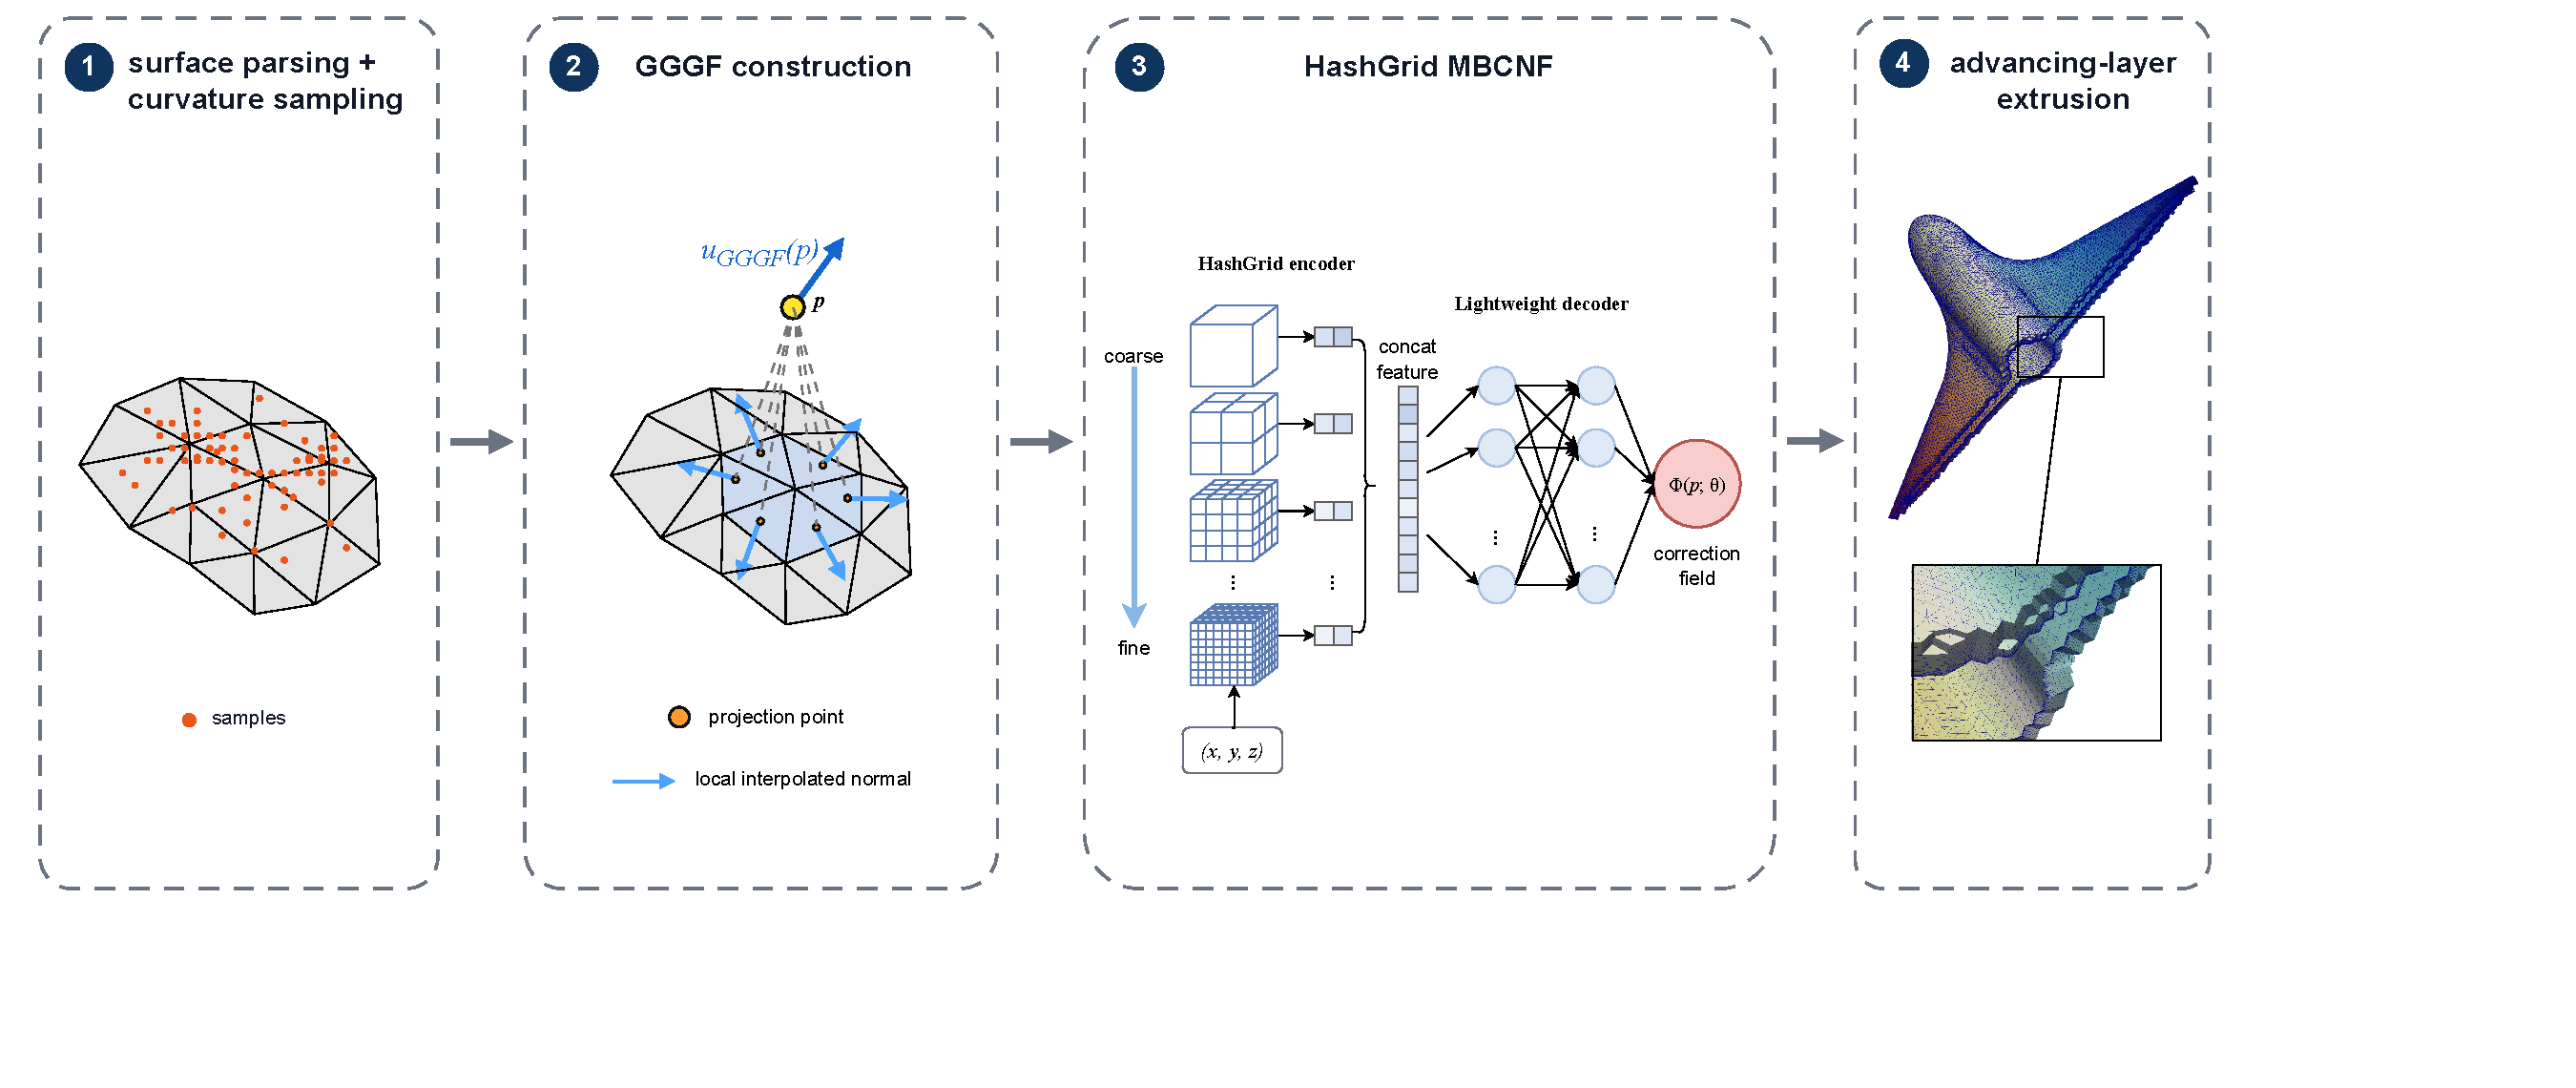
\includegraphics[width=0.5\textwidth]{figs/6new/pip.pdf}
    \caption{\label{fig:pip}
    Pipeline of 3D Anisotropic Mesh Generation.}
\end{figure}
Our paper proposes an automated framework for generating 3D anisotropic, semi-structured boundary layer meshes. 
Diverging from the conventional paradigm of global Partial Differential Equation (PDE) solvers, this framework adopts a neural field generation approach driven by boundary information. 
This section outlines the complete, highly automated workflow for generating 3D anisotropic meshes for specific geometries.
An overview of the proposed pipeline is presented in Fig. \ref{fig:pip}.
\begin{enumerate}
    \item \textbf{3D Surface Parsing and Spatial Discretization:}Read a 3D volume mesh file containing a single boundary layer, and utilize spatial volume mesh generation alongside curvature-weight-driven surface sampling to generate the set of physical spatial sampling points for subsequent neural network training.
    \item \textbf{Construction of the Global Geometric Guidance Field (GGGF):}By leveraging KD-Tree acceleration coupled with local barycentric coordinate interpolation, a robust Global Geometric Guidance Field is constructed within the computational domain. This field provides high-quality geometric priors to guide the neural network training.
    \item \textbf{Training of the Multiresolution Boundary-Constrained Neural Field (MBCNF):}We construct a boundary-informed neural field equipped with a multiresolution HashGrid encoder to predict the corrective growth direction over the 3D computational domain. Each spatial point is first normalized within the geometry-dependent bounding box and encoded by a hierarchy of learnable HashGrid levels, allowing the network to efficiently capture localized CAD features such as sharp curvature variations and concave-convex transitions. The concatenated multiscale HashGrid features are then decoded by a lightweight MLP to produce a residual correction field.

    To ensure that the high local capacity of the multiresolution HashGrid encoder does not introduce non-physical grid-scale perturbations, the training objective combines boundary cosine similarity with a Laplacian smoothing loss. 
    The latter acts as an explicit spatial smoothness prior and suppresses localized high-frequency microstructures that may arise from hash collisions or weakly constrained interior regions. 
    In addition, a fifth-order smootherstep interpolation kernel is adopted in the HashGrid encoder to provide $C^2$-compatible transitions across grid cells, making the encoded field better suited for second-order Laplacian regularization. 
    Finally, the learned residual field is coupled with the global geometric guidance field through a distance-dependent modulation function, so that the correction vanishes near the wall and gradually becomes active away from the boundary. 
    This formulation preserves the near-wall orthogonality constraint while enabling the combined field to provide smooth, locally adaptive boundary-layer growth directions throughout the global domain.
    \item \textbf{High-Quality 3D Advancing Layer Generation:}The trained MBCNF is used to evaluate the residual correction field, which is combined with the GGGF to obtain the final predicted growth directions for boundary-layer extrusion. By dynamically adjusting the distance-based weighting between the learned residual correction and the geometric boundary prior, the method effectively steers the layer-by-layer extrusion of the prismatic boundary layer mesh.
\end{enumerate}

\subsection{\label{sec:level1-3}Curvature-Driven Spatial Sampling Strategy}
To empower the neural network to effectively capture sharp and intricate geometric features, and to synergize with the subsequent Laplacian smoothing loss function, a comprehensive non-uniform spatial sampling mechanism is established.
    
    The sampling procedure begins with the discretization of the physical domain.
    Utilizing the tetrahedral tessellation techniques provided by the TetGen library, a discrete point sequence is generated within the annular domain ($\Omega$) bounded by the inner and outer boundaries. Concurrently, a hierarchical point distribution is imposed along the wall-normal direction according to the final boundary-layer growth parameters, including the first-layer thickness, growth rate, and total number of layers. Specifically, sampling points are placed at selected cumulative layer heights along the inner-surface normals, so that they cover the entire boundary-layer growth region used in the subsequent advancing-layer generation. This domain-wide coverage provides effective supervision for the neural field throughout the extrusion region, enabling the network to learn appropriate growth-direction vectors at different wall-normal distances and to produce stable vector predictions during the complete boundary-layer growth process.
    
    After the spatial point set is constructed, geometric singularities are identified to guide non-uniform sampling.
    Regions exhibiting drastic geometric variations are identified by evaluating the discrete curvature. For the target sampling point sets located on the inner boundary and within the annular physical domain $\Omega$, this curvature is assessed utilizing the normal vector set $\mathbf{N}_{adj}$ from their $k$ adjacent faces (for spatial points within $\Omega$, the adjacent faces are determined via mapping to the nearest inner boundary).
    
    The detected geometric variation is then converted into an importance weight for probabilistic sampling.
    As shown in the formula \ref{eq:sampling_weight}, a sampling weight $W_i$ is defined to quantitatively represent these geometric singularities. During the subsequent sampling phase for the point sets on the inner boundary and within the domain $\Omega$, a probabilistic sampling strategy is executed based on these computed weights.
    \begin{equation}
        W_i = 1.0 - \min_{n \in N_{\text{adj}}} (\mathbf{n} \cdot \mathbf{n}_{\text{ref}}) + \epsilon
    \label{eq:sampling_weight}
    \end{equation}
    A regularization constant is incorporated into the formulation to strictly prevent zero weights, thereby ensuring comprehensive sampling coverage across the entire global domain.

    Finally, the outer boundary is handled separately. A uniform sampling approach is adopted for this boundary to maintain the baseline geometric constraints.
% \subsection{\label{sec:level2}Global Geometric Guidance Field}
% To alleviate the training burden on the neural network, we construct a Multiresolution Boundary-Constrained Neural Field (MBCNF), denoted as $\mathbf{u}_{mbcnf}$, which is intrinsically defined by the normal vectors of the inner boundary ($\mathbf{n}_{inner}$). This field dynamically modulates the strength of spatial constraints via a distance function $f(d)$. Specifically, it imposes a strong orthogonal prior in the near-wall region to guarantee the quality of the generated boundary layer. Conversely, in the far-field region, it serves as a baseline field that couples with the residual field predicted by the neural network to asymptotically approach the target direction of the outer boundary. This formulation bypasses the necessity for the model to approximate complex geometric manifold features from scratch. Instead, it casts the prediction objective into a residual learning paradigm, wherein the neural network is solely tasked with learning and predicting the local residuals between the geometric prior field and the target field.

% The construction procedure for $\mathbf{u}_{mbcnf}$ is detailed as follows: For an arbitrary spatial point $\mathbf{p}$ located on or outside the inner boundary, a KD-Tree spatial index is employed to retrieve its $K$ nearest triangular faces on the inner boundary. We compute the exact projection of point $\mathbf{p}$ onto each respective face along with its corresponding barycentric coordinates. Subsequently, incorporating the Euclidean distances between point $\mathbf{p}$ and these $K$ adjacent faces, an Inverse Distance Weighting (IDW) scheme is applied to seamlessly fuse the discrete normal information from these faces. This procedure establishes a globally continuous initial reference field. Finally, by superimposing the corrective vector predicted by the neural network onto this initial field, the definitive growth normal vector is obtained (as formulated in Section 3.4).
\subsection{\label{sec:level1-4}Global Geometric Guidance Field}

\begin{figure}[H]
    \centering
    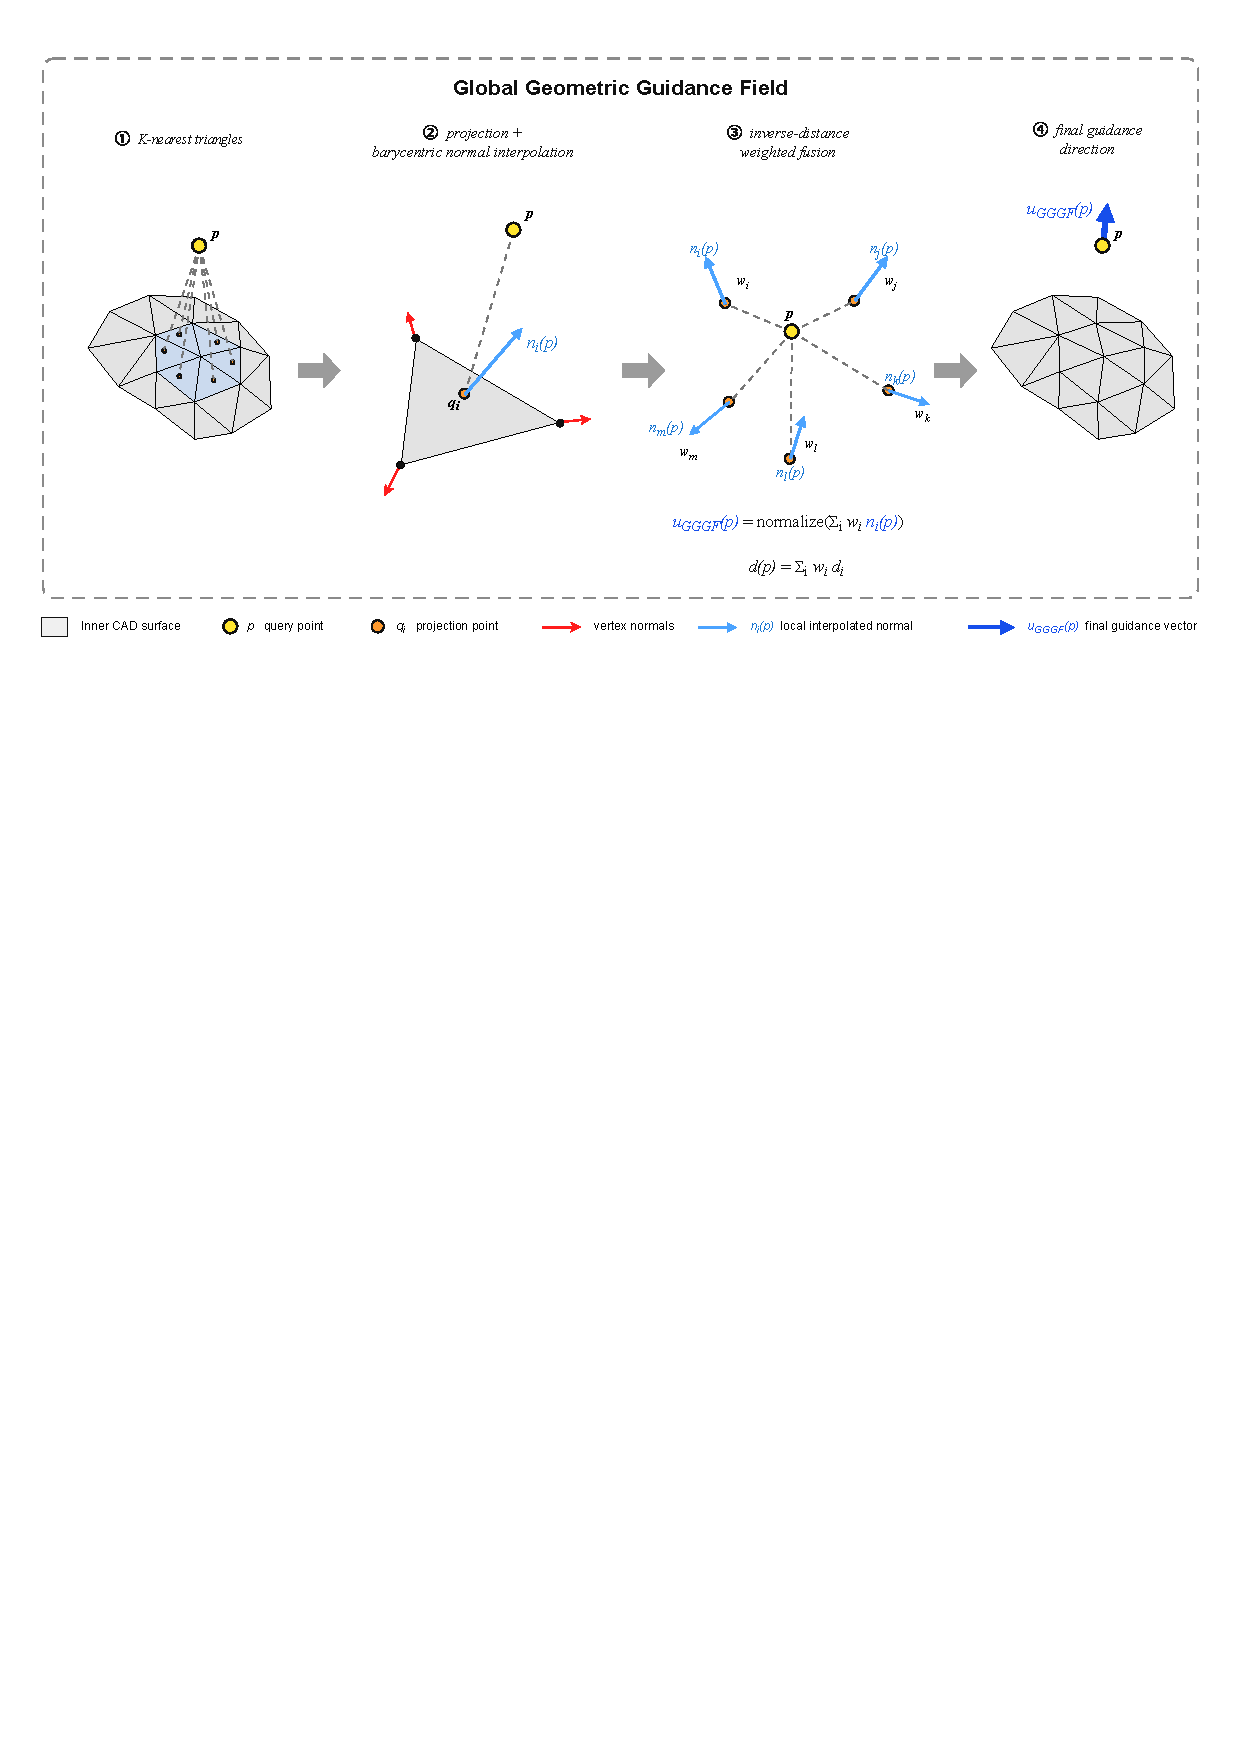
\includegraphics[width=0.5\textwidth]{figs/net/gggf.pdf}
    \caption{\label{fig:gggf}
    Global Geometric Guidance Field.}
    \end{figure}

To reduce the learning burden of the neural network and to explicitly embed reliable CAD boundary information into the prediction process, we construct a Global Geometric Guidance Field (GGGF) from the inner boundary surface.
The GGGF serves as a geometry-driven prior for the boundary-layer growth direction. Instead of requiring the neural network to infer the entire spatial direction field from sparse boundary supervision alone, this field provides an explicit reference direction derived from the surface-normal distribution of the CAD geometry.
The neural network is therefore guided to learn only the residual correction with respect to this geometric prior, as detailed in the subsequent multiresolution boundary-constrained neural field formulation.

The complete construction procedure is summarized in Algorithm~\ref{alg:gggf_procedure}.
For an arbitrary query point $\mathbf{p}$ located on or outside the inner boundary, the method first retrieves its neighboring triangular faces on the inner surface through a spatial tree index.
In the implementation, the number of neighboring faces is set to $K=20$.
For each retrieved triangle, the closest projection point from $\mathbf{p}$ to the triangle is computed.
The barycentric coordinates of this projected point are then used to interpolate the vertex normals of the corresponding triangle, yielding a local surface-normal estimate associated with that triangle.
This triangle-wise interpolation is important for CAD-derived surface meshes because it avoids directly using discontinuous face normals and provides a smoother local estimate of the wall-normal direction.

Let $\mathbf{q}_{i}$ denote the closest projection of $\mathbf{p}$ onto the $i$-th neighboring triangle, and let $d_i=\|\mathbf{p}-\mathbf{q}_{i}\|_2$ be the corresponding projection distance. The interpolated unit normal obtained from the barycentric coordinates on this triangle is denoted as $\mathbf{n}_{i}(\mathbf{p})$. The final guidance direction is obtained by inverse-distance weighting:
\begin{equation}
    w_i(\mathbf{p}) =
    \frac{(d_i+\epsilon)^{-1}}
    {\sum_{j=1}^{K}(d_j+\epsilon)^{-1}},
    \label{eq:gggf_weight}
\end{equation}
\begin{equation}
    \mathbf{u}_{gggf}(\mathbf{p}) =
    \frac{\sum_{i=1}^{K} w_i(\mathbf{p}) \mathbf{n}_{i}(\mathbf{p})}
    {\left\|\sum_{i=1}^{K} w_i(\mathbf{p}) \mathbf{n}_{i}(\mathbf{p})\right\|_2+\epsilon}.
    \label{eq:gggf_normal}
\end{equation}
The distance variable used by the subsequent boundary modulation is computed consistently as the weighted projection distance:
\begin{equation}
    d(\mathbf{p}) = \sum_{i=1}^{K} w_i(\mathbf{p}) d_i .
    \label{eq:gggf_distance}
\end{equation}
Compared with a single nearest-face projection, this $K$-neighbor inverse-distance fusion is less sensitive to local triangulation irregularities or isolated noisy faces, while still preserving the local geometric characteristics of high-curvature and concave-convex regions. As a result, the GGGF provides a stable and physically meaningful baseline direction for the subsequent neural residual learning stage.

\begin{center}
    \begin{minipage}{0.96\columnwidth}
    \refstepcounter{algorithm}
    \label{alg:gggf_procedure}
    \hrule height 0.8pt
    \vspace{0.45em}
    \noindent\textbf{Algorithm \thealgorithm. Construction of the Global Geometric Guidance Field}

    \vspace{0.35em}
    \small
    \noindent\textbf{Input:}\\[-0.2em]
    \begin{tabular}{@{\hspace{2.4em}}l@{}}
        Inner boundary triangular mesh $\mathcal{M}_{in}=(V,F)$;\\
        Vertex normal set $\mathcal{N}_v$;\\
        Query point set $P=\{\mathbf{p}_i\}_{i=1}^{N_p}$;\\
        Number of neighboring triangles $K$;\\
        Numerical constant $\epsilon$.
    \end{tabular}

    \noindent\textbf{Output:}\\[-0.2em]
    \begin{tabular}{@{\hspace{2.4em}}l@{}}
        Weighted distance set $D=\{d(\mathbf{p}_i)\}_{i=1}^{N_p}$;\\
        Global Geometric Guidance Field $U_{GGGF}=\{\mathbf{u}_{gggf}(\mathbf{p}_i)\}_{i=1}^{N_p}$.
    \end{tabular}

    \vspace{0.25em}
    \begin{algorithmic}[1]
        \STATE Build a spatial triangle search tree for the triangular faces of $\mathcal{M}_{in}$.

        \FOR{each query point $\mathbf{p}_i \in P$}
            \STATE Retrieve the $K$ nearest triangular faces $\{T_{i,k}\}_{k=1}^{K}$ from the search tree.
            \STATE If fewer than $K$ faces are found, repeat the last valid face index until $K$ candidates are obtained.

            \FOR{each neighboring triangle $T_{i,k}$}
                \STATE Compute the closest projection point and projection distance:
                \[
                    \mathbf{q}_{i,k}=\Pi_{T_{i,k}}(\mathbf{p}_i),
                    \qquad
                    d_{i,k}=\|\mathbf{p}_i-\mathbf{q}_{i,k}\|_2 .
                \]
                \STATE Compute the barycentric coordinates $\boldsymbol{\beta}_{i,k}=(\beta_{i,k}^{1},\beta_{i,k}^{2},\beta_{i,k}^{3})$ of $\mathbf{q}_{i,k}$ on $T_{i,k}$.
                \STATE Interpolate and normalize the local normal:
                \[
                    \mathbf{n}_{i,k}
                    =
                    \frac{
                    \sum_{\ell=1}^{3}\beta_{i,k}^{\ell}\mathbf{n}_{i,k}^{\ell}
                    }{
                    \left\|\sum_{\ell=1}^{3}\beta_{i,k}^{\ell}\mathbf{n}_{i,k}^{\ell}\right\|_2+\epsilon
                    } .
                \]
            \ENDFOR

            \STATE Compute inverse-distance weights:
            \[
                w_{i,k}
                =
                \frac{(d_{i,k}+\epsilon)^{-1}}
                {\sum_{m=1}^{K}(d_{i,m}+\epsilon)^{-1}} .
            \]

            \STATE Compute the weighted projection distance:
            \[
                d(\mathbf{p}_i)
                =
                \sum_{k=1}^{K}w_{i,k}d_{i,k}.
            \]

            \STATE Fuse and normalize the local normals to obtain the GGGF direction:
            \[
                \mathbf{u}_{gggf}(\mathbf{p}_i)
                =
                \frac{
                \sum_{k=1}^{K}w_{i,k}\mathbf{n}_{i,k}
                }{
                \left\|\sum_{k=1}^{K}w_{i,k}\mathbf{n}_{i,k}\right\|_2+\epsilon
                } .
            \]

            \STATE Store $d(\mathbf{p}_i)$ in $D$ and $\mathbf{u}_{gggf}(\mathbf{p}_i)$ in $U_{GGGF}$.
        \ENDFOR

        \RETURN $D$ and $U_{GGGF}$.
    \end{algorithmic}
    \vspace{0.2em}
    \hrule height 0.8pt
    \end{minipage}
\end{center}

\subsection{\label{sec:level1-5}Multiresolution Boundary-Constrained Neural Field}

\begin{figure*}
    \centering
    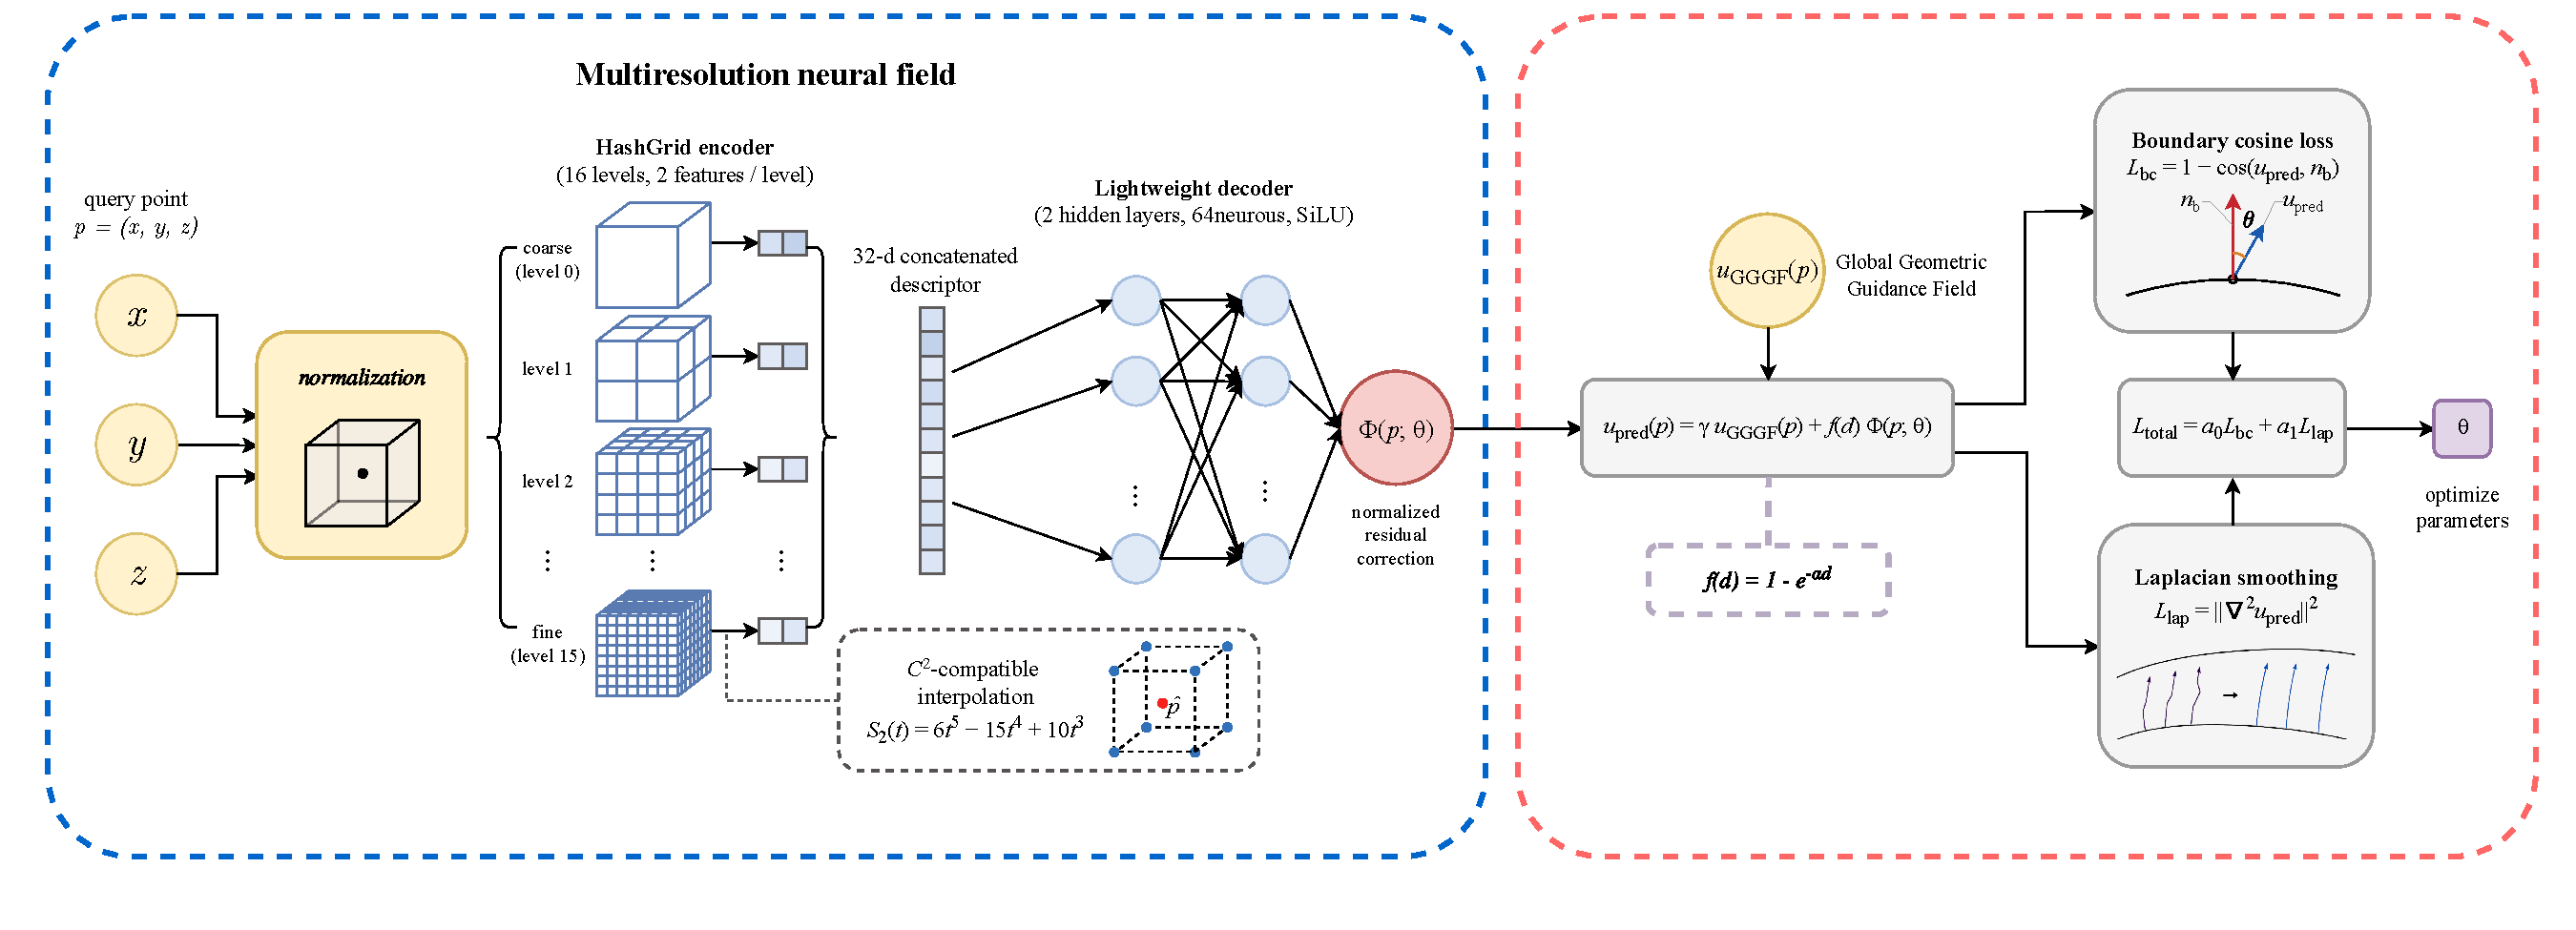
\includegraphics[width=1\textwidth]{figs/net/net.pdf}
    \caption{Multiresolution Boundary-Constrained Neural Field for Anisotropic Boundary-Layer Mesh Generation}
    \label{fig:net}
\end{figure*}
Traditional coordinate-based neural networks based on Multi-Layer Perceptrons (MLPs) are often limited by their inherent spectral bias, which makes them inefficient in resolving localized high-frequency geometric variations in complex CAD-derived boundary-layer domains. 
To overcome this limitation, we introduce a Boundary-Constrained Neural Field equipped with a multiresolution HashGrid encoder. 
Fig. \ref{fig:net} shows the overall architecture of the neural field.
Instead of directly mapping Cartesian coordinates to growth directions using a deep global MLP, each spatial point $\mathbf{p}=(x,y,z)$ is first normalized within a geometry-dependent bounding box and encoded by a hierarchy of learnable HashGrid levels.
These hierarchical HashGrid levels decompose the spatial representation into multi-scale local basis functions, thereby improving the model's ability to represent sharp curvature variations, concave-convex transitions, and other localized CAD features.

In our implementation, the HashGrid encoder contains 16 resolution levels, with two trainable feature channels at each level.
For each level, the eight neighboring lattice vertices of the query point are indexed through a spatial hash function, and the interpolated features from all levels are concatenated into a compact 32-dimensional multiscale descriptor.
This descriptor is then decoded by a lightweight MLP with two 64-neuron hidden layers and SiLU activations to predict a residual correction vector.
By transferring most of the local geometric representation burden from the decoder to the multiresolution HashGrid levels, the proposed architecture captures complex local geometric features without requiring an excessively deep global MLP.

To prevent hash-induced numerical oscillations, the HashGrid-encoded neural field is further regularized by a smoothness-aware formulation.
Although the multiresolution HashGrid encoder provides strong local representational capacity, it also requires careful regularization. As discussed in the Instant-NGP work, fine HashGrid levels inevitably involve hash collisions, where different spatial locations may share the same hash-table entry. The multiresolution HashGrid hierarchy helps the network resolve most collision-induced ambiguity during optimization, but residual collision artifacts may still appear as grid-scale microstructures or localized high-frequency perturbations. 
In boundary-layer mesh generation, such perturbations are particularly harmful: even a small directional error in the predicted vector field can be repeatedly accumulated during layer-by-layer advancing-layer integration, leading to warped prism edges, local depressions, or degradation of orthogonality in deeper layers.

To address this issue, we introduce a Laplacian smoothing loss as an explicit spatial smoothness prior for the HashGrid-encoded neural field.
The loss penalizes the squared magnitude of the second-order differential operator, $\nabla^2 \mathbf{u}$, evaluated by finite differences over sampled interior points.
This term suppresses localized high-frequency oscillations that are not fully constrained by the boundary cosine losses, especially in regions away from the inner wall where the direct boundary supervision becomes weaker.
In this way, the model retains the expressive advantage of the HashGrid encoder while preventing its high-capacity local representation from producing physically inconsistent directional fluctuations.

To further make the encoded field compatible with Laplacian regularization, we replace the conventional linear interpolation used in standard HashGrid encoders with the fifth-order smootherstep kernel,
    \begin{equation}
        S_2(t)=6t^5-15t^4+10t^3 .
        \label{eq:smootherstep}
    \end{equation}
Linear interpolation only guarantees function-value continuity and introduces first-derivative discontinuities at grid-cell boundaries, which is undesirable for a vector field constrained by a second-order differential operator.
Cubic smoothstep improves first-order smoothness, but its second derivative remains discontinuous across cell boundaries.
In contrast, the fifth-order smootherstep has zero first- and second-order derivatives at both endpoints, which reduces derivative discontinuities at cell boundaries and improves the stability of finite-difference Laplacian evaluation.
Higher-order smoothstep kernels could provide stronger smoothness, but they would increase computational cost and may over-smooth the localized high-frequency geometric details that the HashGrid encoder is designed to capture.
Therefore, the fifth-order smootherstep is selected as a balanced interpolation scheme: it suppresses grid-boundary artifacts and derivative discontinuities while preserving the local representational capacity required for complex CAD boundary-layer mesh generation.

The decoded residual field is not used directly as an unconstrained growth direction.
Instead, the final growth-direction prediction is re-parameterized as a boundary-informed combination of the geometric prior and the learned residual correction, in which the learned correction is coupled with the Global Geometric Guidance Field:
    \begin{equation}
        \mathbf{u}_{pred}(\mathbf{p}) =
        \gamma \mathbf{u}_{gggf}(\mathbf{p}) +
        f(d)\Phi(\mathbf{p};\theta).
        \label{eq:u_pred}
    \end{equation}
Here, $\mathbf{u}_{gggf}(\mathbf{p})$ denotes the Global Geometric Guidance Field constructed by surface-normal projection and inverse-distance interpolation, $\Phi(\mathbf{p};\theta)$ is the residual correction predicted by the HashGrid-encoded neural network, and $\gamma$ controls the contribution of the geometric prior. 
(\(\gamma\) is set to 1.0 in all experiments)
The distance modulation function is defined as
    \begin{equation}
        f(d)=1-\exp(-\alpha d),
        \label{eq:distance_modulation}
    \end{equation}
where $d=d(\mathbf{p})$ is the weighted projection distance to the inner boundary computed from the GGGF construction and $\alpha$ controls the decay rate.

As $d \to 0$, $f(d)$ smoothly approaches zero, forcing the residual correction to vanish near the wall. Consequently, the predicted direction degenerates to the boundary-consistent geometric prior, which imposes the near-wall orthogonality constraint in a hard manner.
Away from the wall, $f(d)$ increases and allows the residual field to compensate for local deviations between the projected inner-boundary normal field and the desired outer-boundary direction.
This formulation reduces the learning burden of the neural network by shifting the prediction target from a complex full-scale vector field to a boundary-constrained residual field, producing a smooth and locally adaptive growth-direction field suitable for robust anisotropic boundary-layer mesh generation.

% \subsection{\label{sec:level2}Loss Functions}
% \begin{itemize}
%     \item \textbf{Boundary Cosine Loss:}o quantify the directional discrepancy between the predicted vector field and the target normal vectors, a weighted cosine similarity metric is employed as the geometric boundary loss:
%     \begin{equation}
%         L_{BC} = \int_{\partial\Omega} \left( 1 - \frac{\mathbf{u}_{pred} \cdot \mathbf{n}_{target}}{\|\mathbf{u}_{pred}\| \|\mathbf{n}_{target}\|} \right) d\Gamma
%     \end{equation}
%     \item \textbf{Laplacian Smoothing Loss:}To prevent the intersection of internal field lines and the formation of singularities, thereby ensuring a seamless geometric transition of the boundary layer mesh from the inner to the outer boundary, a physical regularization term based on the finite difference operator, $\nabla^2 \mathbf{u}$, is introduced. This term rigorously enforces a spatial smoothness constraint across the vector field and is efficiently executed via large-scale parallel finite difference computations on the GPU.
% \end{itemize}
\subsection{\label{sec:level1-6}Loss Functions}

The training objective is designed to simultaneously enforce boundary-direction consistency and interior-field smoothness.
Since the boundary-layer mesh is generated by advancing nodes along the predicted vector field, both the angular accuracy and the spatial regularity of this field directly affect the orthogonality and robustness of the resulting prismatic layers.
The total loss is defined as
\begin{equation}
    \mathcal{L}_{total}
    =
    \lambda_{in}\mathcal{L}_{in}
    +
    \lambda_{out}\mathcal{L}_{out}
    +
    \lambda_{s}\mathcal{L}_{smooth},
    \label{eq:total_loss}
\end{equation}
where $\mathcal{L}_{in}$ and $\mathcal{L}_{out}$ denote the inner- and outer-boundary cosine losses, respectively (see Fig. \ref{fig:anglelossf}),
 and $\mathcal{L}_{smooth}$ denotes the Laplacian smoothing loss imposed on the HashGrid-encoded residual field.

\begin{figure}[H]
    \centering
    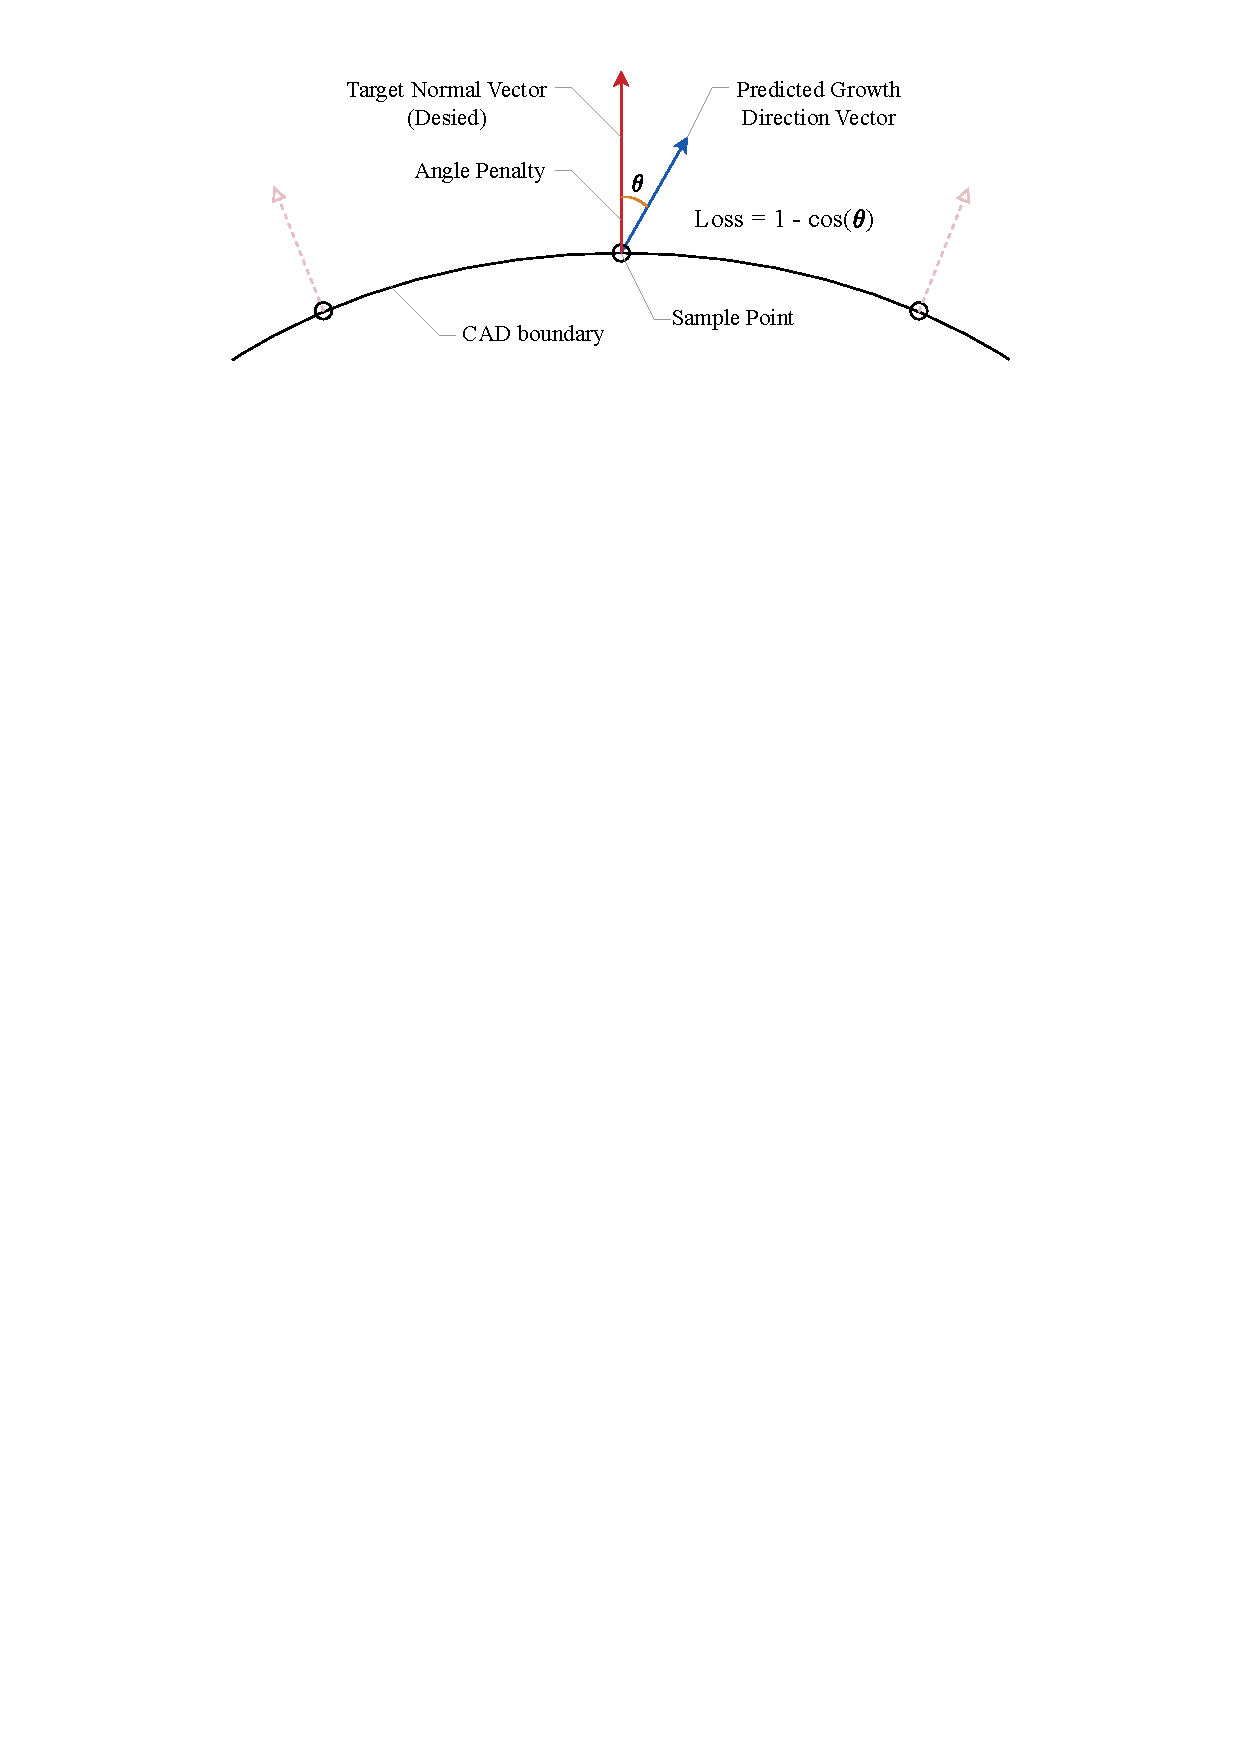
\includegraphics[width=0.4\textwidth]{figs/net/angle.pdf}
    \caption{\label{fig:anglelossf}
    Inner/Outer boundary cosine loss.}
    \end{figure}

    The inner-boundary loss imposes a strong near-wall directional constraint.
    For points sampled on the inner boundary, the residual correction predicted by the HashGrid-encoded neural network is required to align with the target inner-boundary normals.
    This loss is written as
    \begin{equation}
        \mathcal{L}_{in}
        =
        \frac{1}{N_{in}}
        \sum_{i=1}^{N_{in}}
        \left(
        1-
        \frac{
        \Phi(\mathbf{p}^{in}_i;\theta)\cdot \mathbf{n}^{in}_i
        }{
        \left\|\Phi(\mathbf{p}^{in}_i;\theta)\right\|_2
        \left\|\mathbf{n}^{in}_i\right\|_2+\epsilon
        }
        \right),
        \label{eq:loss_inner}
    \end{equation}
    where $\mathbf{p}^{in}_i$ denotes the $i$-th inner-boundary sample, $\mathbf{n}^{in}_i$ is the corresponding target wall-normal vector, and $\epsilon$ is a small numerical constant. This term is assigned the dominant weight in training because the first few boundary layers are highly sensitive to the accuracy of the wall-normal direction. Preserving near-wall orthogonality is therefore treated as the primary geometric requirement.

    The outer-boundary loss constrains the composite predicted direction at the outer boundary.
    Unlike the inner-boundary term, this loss is applied to the boundary-informed field obtained by combining the Global Geometric Guidance Field with the neural residual correction:
    \begin{equation}
        \mathbf{u}_{pred}(\mathbf{p})
        =
        \gamma\mathbf{u}_{gggf}(\mathbf{p})
        +
        f(d)\Phi(\mathbf{p};\theta).
        \label{eq:loss_upred}
    \end{equation}
    The outer-boundary loss is then defined as
    \begin{equation}
        \mathcal{L}_{out}
        =
        \frac{1}{N_{out}}
        \sum_{i=1}^{N_{out}}
        \left(
        1-
        \frac{
        \mathbf{u}_{pred}(\mathbf{p}^{out}_i)\cdot \mathbf{n}^{out}_i
        }{
        \left\|\mathbf{u}_{pred}(\mathbf{p}^{out}_i)\right\|_2
        \left\|\mathbf{n}^{out}_i\right\|_2+\epsilon
        }
        \right),
        \label{eq:loss_outer}
    \end{equation}
    where $\mathbf{p}^{out}_i$ denotes the $i$-th outer-boundary sample and $\mathbf{n}^{out}_i$ is the corresponding target direction. This term guides the learned vector field to smoothly transition from the inner-wall normal prior toward the desired outer-boundary direction.
    In the implementation, $\lambda_{out}$ is set smaller than $\lambda_{in}$, reflecting its role as a far-field guidance term rather than a dominant near-wall constraint.

    Both boundary losses are formulated using cosine similarity rather than a direct Euclidean vector loss.
    This choice is motivated by the nature of boundary-layer mesh generation: the advancing-layer procedure depends primarily on the direction of the vector field, while the step length is independently controlled by the prescribed layer thickness.
    A cosine loss explicitly penalizes angular misalignment and is insensitive to irrelevant magnitude variations, making it more suitable for enforcing normal-direction consistency than a standard $L_2$ loss.
    \begin{figure}[H]
        \centering
        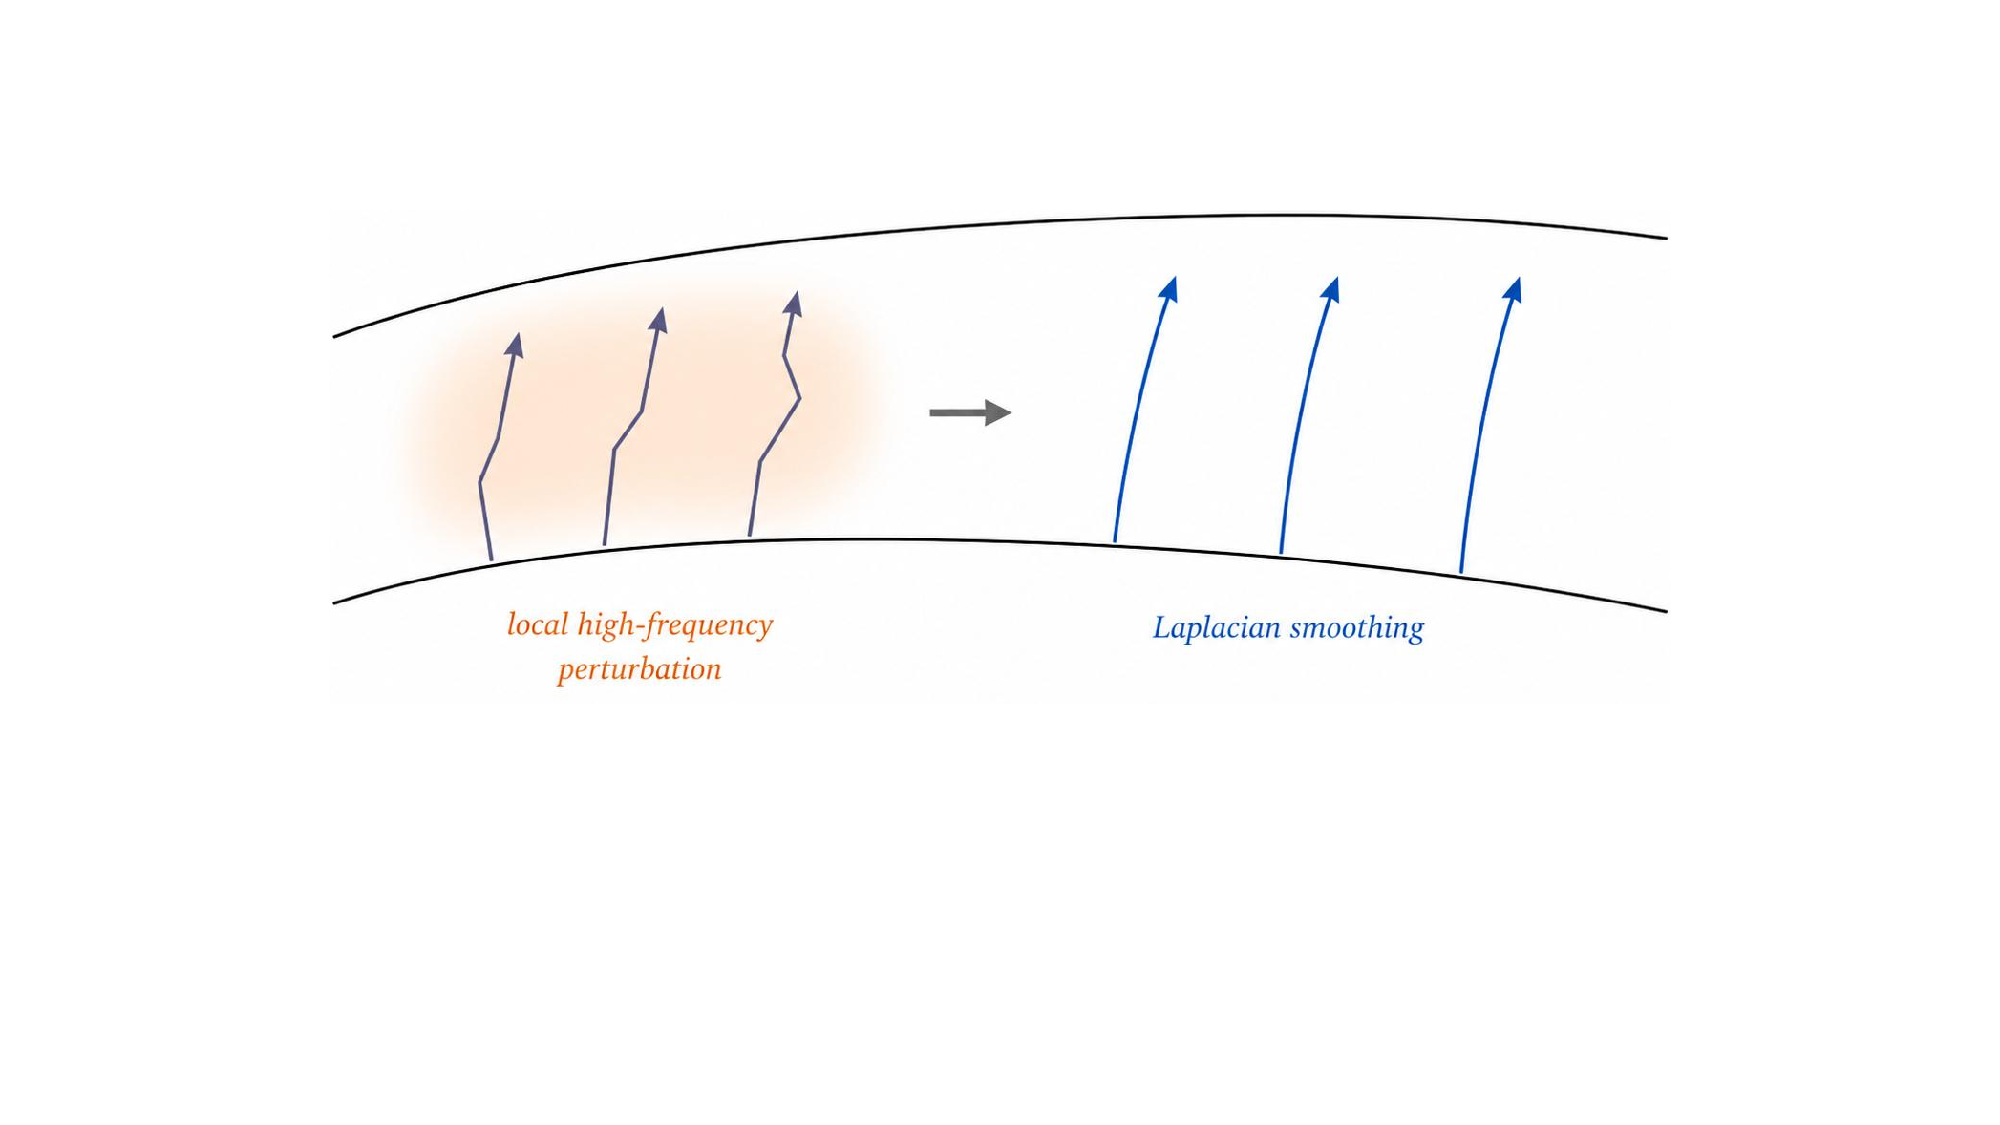
\includegraphics[width=0.4\textwidth]{figs/net/laplace_smooth.pdf}
        \caption{\label{fig:laplacef}
        Laplacian smoothing loss.}
    \end{figure}
    To regularize the interior vector field, a Laplacian smoothing loss is introduced over randomly sampled domain points. 
    The corresponding smoothing mechanism is illustrated in Fig. \ref{fig:laplacef}.
    This term penalizes the squared magnitude of the second-order spatial variation of the residual field predicted by the HashGrid-encoded neural network:
    \begin{equation}
        \mathcal{L}_{smooth}
        =
        \frac{1}{N_{\Omega}}
        \sum_{i=1}^{N_{\Omega}}
        \left\|
        \nabla^2 \Phi(\mathbf{p}^{\Omega}_i;\theta)
        \right\|_2^2,
        \label{eq:loss_smooth}
    \end{equation}
    where $\mathbf{p}^{\Omega}_i$ denotes an interior sample point in the computational domain. In practice, the Laplacian operator is approximated by central finite differences along the three coordinate directions:
    \begin{equation}
        \nabla^2 \Phi(\mathbf{p};\theta)
        \approx
        \sum_{k=1}^{3}
        \frac{
        \Phi(\mathbf{p}+\delta\mathbf{e}_k;\theta)
        -
        2\Phi(\mathbf{p};\theta)
        +
        \Phi(\mathbf{p}-\delta\mathbf{e}_k;\theta)
        }{\delta^2},
        \label{eq:laplacian_fd}
    \end{equation}
    where $\mathbf{e}_k$ is the unit vector along the $k$-th coordinate direction and $\delta$ is the finite-difference step size.

    The use of this loss is particularly important for the multiresolution HashGrid encoder. Although the HashGrid encoder provides strong local representational capacity, hash collisions and weak interior supervision may produce localized high-frequency perturbations.
    Such perturbations can accumulate during layer-by-layer mesh advancement and lead to distorted prism elements in deeper layers.
    The Laplacian smoothing loss suppresses these non-physical oscillations and encourages the residual field to vary smoothly throughout the computational domain. 
    For GPU efficiency, this term is evaluated on mini-batches of interior samples during training.

\subsection{\label{sec:level1-7}Advancing-Layer Method Mesh Generation}

After the converged growth-direction field $\mathbf{u}_{pred}$ is obtained, the anisotropic boundary-layer mesh is generated by a layer-by-layer advancing procedure.
This stage follows the advancing-layer strategy adopted in boundary-informed anisotropic meshing methods~\cite{anisoMeshNet}, where the learned vector field is used to guide the extrusion of boundary nodes from the wall surface into the computational domain.
In contrast to conventional normal-smoothing-based extrusion, the advancing direction in our method is provided by the final field \(\mathbf{u}_{pred}\), which combines the near-wall geometric prior with the learned residual correction predicted by the trained MBCNF.

Let $\mathbf{p}_{j}^{(i)}$ denote the position of the $j$-th node on the $i$-th advancing front. The node position on the next layer is computed by advancing along the normalized predicted direction:
\begin{equation}
    \mathbf{p}_{j}^{(i+1)}
    =
    \mathbf{p}_{j}^{(i)}
    +
    h_i
    \frac{
    \mathbf{u}_{pred}\left(\mathbf{p}_{j}^{(i)}\right)
    }{
    \left\|
    \mathbf{u}_{pred}\left(\mathbf{p}_{j}^{(i)}\right)
    \right\|_2
    },
    \label{eq:new_point}
\end{equation}
where $h_i$ is the thickness of the $i$-th boundary layer. Following the common geometric-growth setting used in advancing-layer mesh generation, the layer thickness is defined as
\begin{equation}
    h_i = h_0 r^i,
    \label{eq:layer_thickness}
\end{equation}
where $h_0$ is the first-layer thickness and $r$ is the prescribed layer-to-layer growth rate.

Starting from the triangular faces of the inner boundary surface, each active front is advanced according to Eq.~\eqref{eq:new_point}.
Corresponding nodes between two consecutive fronts are connected to form prismatic boundary-layer elements. Repeating this process for a prescribed number of layers yields a structured stack of anisotropic prism elements aligned with the predicted growth-direction field. Therefore, the mesh generation stage inherits the geometric simplicity of the advancing-layer method while replacing the traditional hand-crafted marching normal field with the proposed neural field, enabling boundary-layer extrusion over complex three-dimensional CAD geometries.

\section{\label{sec:level2}Experiments and Results}

\subsection{\label{sec:level2-1}Experimental Setup}

\begin{table*}[!ht]
    \centering
    \caption{Key implementation details of the proposed framework}
    \label{tab:hyperparameters}
    \begin{tabular}{ll}
        \toprule
        \textbf{Parameter} & \textbf{Value} \\
        \midrule
        \multicolumn{2}{l}{\textbf{Multiresolution HashGrid Encoder}} \\
        Input layer neurons & 3 (3D spatial coordinates $x, y, z$)\\
        Output layer neurons & 32 (16 levels $\times$ 2 features per level)\\
        Weight initialization & Uniform distribution\\
        Number of hash levels ($L$) & 16 \\
        Base resolution ($N_{\min}$) & 16 \\
        Maximum resolution ($N_{\max}$) & 512 \\
        Hash table size ($\log_2 T$) & 19 \\
        Feature dimensions per level ($F$) & 2 \\
        \midrule
        \multicolumn{2}{l}{\textbf{Tiny MLP Architecture}} \\
        Input layer neurons&32 (Concatenated multiresolution HashGrid features)\\
        Hidden layers& 2 layers (64, 64 neurons)\\
        Output layer neurons& 3 (residual correction vector)\\
        Activation function & SiLU (Swish)\\
        Weight initialization& Kaiming uniform \\
        \midrule
        \multicolumn{2}{l}{\textbf{Training Hyperparameters}} \\
        Total training epochs & 75000 \\
        Learning rate (HashGrid embeddings) & $3 \times 10^{-3}$ \\
        Learning rate (MLP decoder) & $1 \times 10^{-3}$ \\
        Learning rate scheduler &StepLR (step size=2000, gamma=0.8) \\
        Optimizer &  Adam\\
        Batch size & 4096 \\
        Stopping criteria &Fixed epoch count (75000) \\
        Number of domain points & 10,000 \\
        Number of inner boundary points & 10,000 \\
        Number of outer boundary points & 500 \\
        % $K$-nearest neighbors & 20 \\
        % Exponential decay rate & 20.0 \\
        Device  & NVIDIA RTX 3050Ti GPU / CPU (fallback) \\
        \midrule
        \multicolumn{2}{l}{\textbf{Loss Function Weights}} \\
        Inner boundary weight ($\lambda_{\text{bc\_inner}}$) & 1.0 \\
        Outer boundary weight ($\lambda_{\text{bc\_outer}}$) & 0.001 \\
        Laplacian smoothing weight ($\lambda_{\mathrm{s}}$) & 0.05 \\
        \midrule
        \multicolumn{2}{l}{\textbf{Mesh Generation Parameters}} \\
        Number of layers & 25 \\
        First layer thickness & $5 \times 10^{-5}$ \\
        Growth rate & 1.15 \\
        \bottomrule
    \end{tabular}
\end{table*}


All models were implemented in PyTorch and trained on an NVIDIA RTX 3050Ti GPU (with CPU fallback capability). The proposed neural network architecture consists of two tightly coupled components: a multiresolution HashGrid encoder and a Tiny MLP decoder. Specifically, the HashGrid encoder takes 3D spatial coordinates ($x, y, z$) as input and maps them into a 32-dimensional concatenated feature vector using 16 HashGrid levels, with two feature dimensions at each level. This encoded multiresolution feature vector is subsequently fed into the input layer of the Tiny MLP. The Tiny MLP comprises two hidden layers with 64 neurons each and utilizes the SiLU (Swish) activation function to predict the 3D residual correction vector. 
The core hyperparameters, including loss weights and mesh generation settings, are summarized in Table \ref{tab:hyperparameters}.

Key parameters for the framework were set as follows:

\begin{itemize}
    \item \textbf{Geometric Features:} The K-Nearest Neighbors algorithm used $K = 20$ neighbors to robustly interpolate the target surface normals and calculate the weighted average distance.
    
    \item \textbf{Loss Function:} The composite loss function prioritized geometric accuracy and network stability, with the inner boundary loss assigned a weight of $1.0$ and the outer boundary loss a weight of $0.001$ to ensure strict orthogonality in critical near-body regions. Additionally, a Laplacian smoothing loss weight of $5 \times 10^{-2}$ was incorporated to mitigate local distortions.
    
    \item \textbf{Mesh Generation:} The advancing-layer algorithm was configured to generate $25$ layers with a highly refined initial thickness of $5 \times 10^{-5}$ and a layer-to-layer growth rate of $1.15$.
\end{itemize}

\subsection{\label{sec:level3}Ablation Studies}
To validate the effectiveness of the key components in our proposed method, we designed and conducted three sets of ablation studies.
The three test geometries are denoted as model1, model2, and model3 throughout the ablation studies. Specifically, model1 and model2 correspond to two aircraft geometries, while model3 corresponds to the Stanford Bunny model.

\subsubsection{\label{sec:level3-1}Impacts of Boundary Cosine Loss}

To evaluate the role of boundary-direction supervision, we conducted a comparative ablation study on model1 using three boundary-direction loss formulations: a unit-norm penalty, a squared chord-length loss, and the proposed boundary cosine loss. 
In this ablation study, the compared loss formulations are applied to the boundary-direction supervision used on both the inner and outer boundaries. Since the supervised quantity differs between the two boundaries, we introduce a unified notation for clarity. Let \(\mathcal{B}=\mathcal{B}_{in}\cup\mathcal{B}_{out}\) denote the set of boundary samples used for directional supervision, with \(N_b=|\mathcal{B}|\). For each sample \(\mathbf{p}_i\in\mathcal{B}\), the supervised direction is denoted as \(\mathbf{q}_i\), where \(\mathbf{q}_i=\Phi(\mathbf{p}_i;\theta)\) for inner-boundary samples and \(\mathbf{q}_i=\mathbf{u}_{pred}(\mathbf{p}_i)\) for outer-boundary samples. The corresponding target direction is denoted as \(\mathbf{n}_i\).
With this notation, the three compared boundary-direction losses can be expressed in a consistent form.

As shown in Fig. \ref{fig:angleloss_losscurve}, the top row compares the generated prismatic boundary-layer meshes, while the bottom row reports the corresponding training convergence histories. The results indicate that directly constraining angular consistency is essential for obtaining stable and physically meaningful boundary-layer growth directions.
\begin{figure*}[t]
    \centering

    \begin{subfigure}[b]{0.31\textwidth}
        \centering
        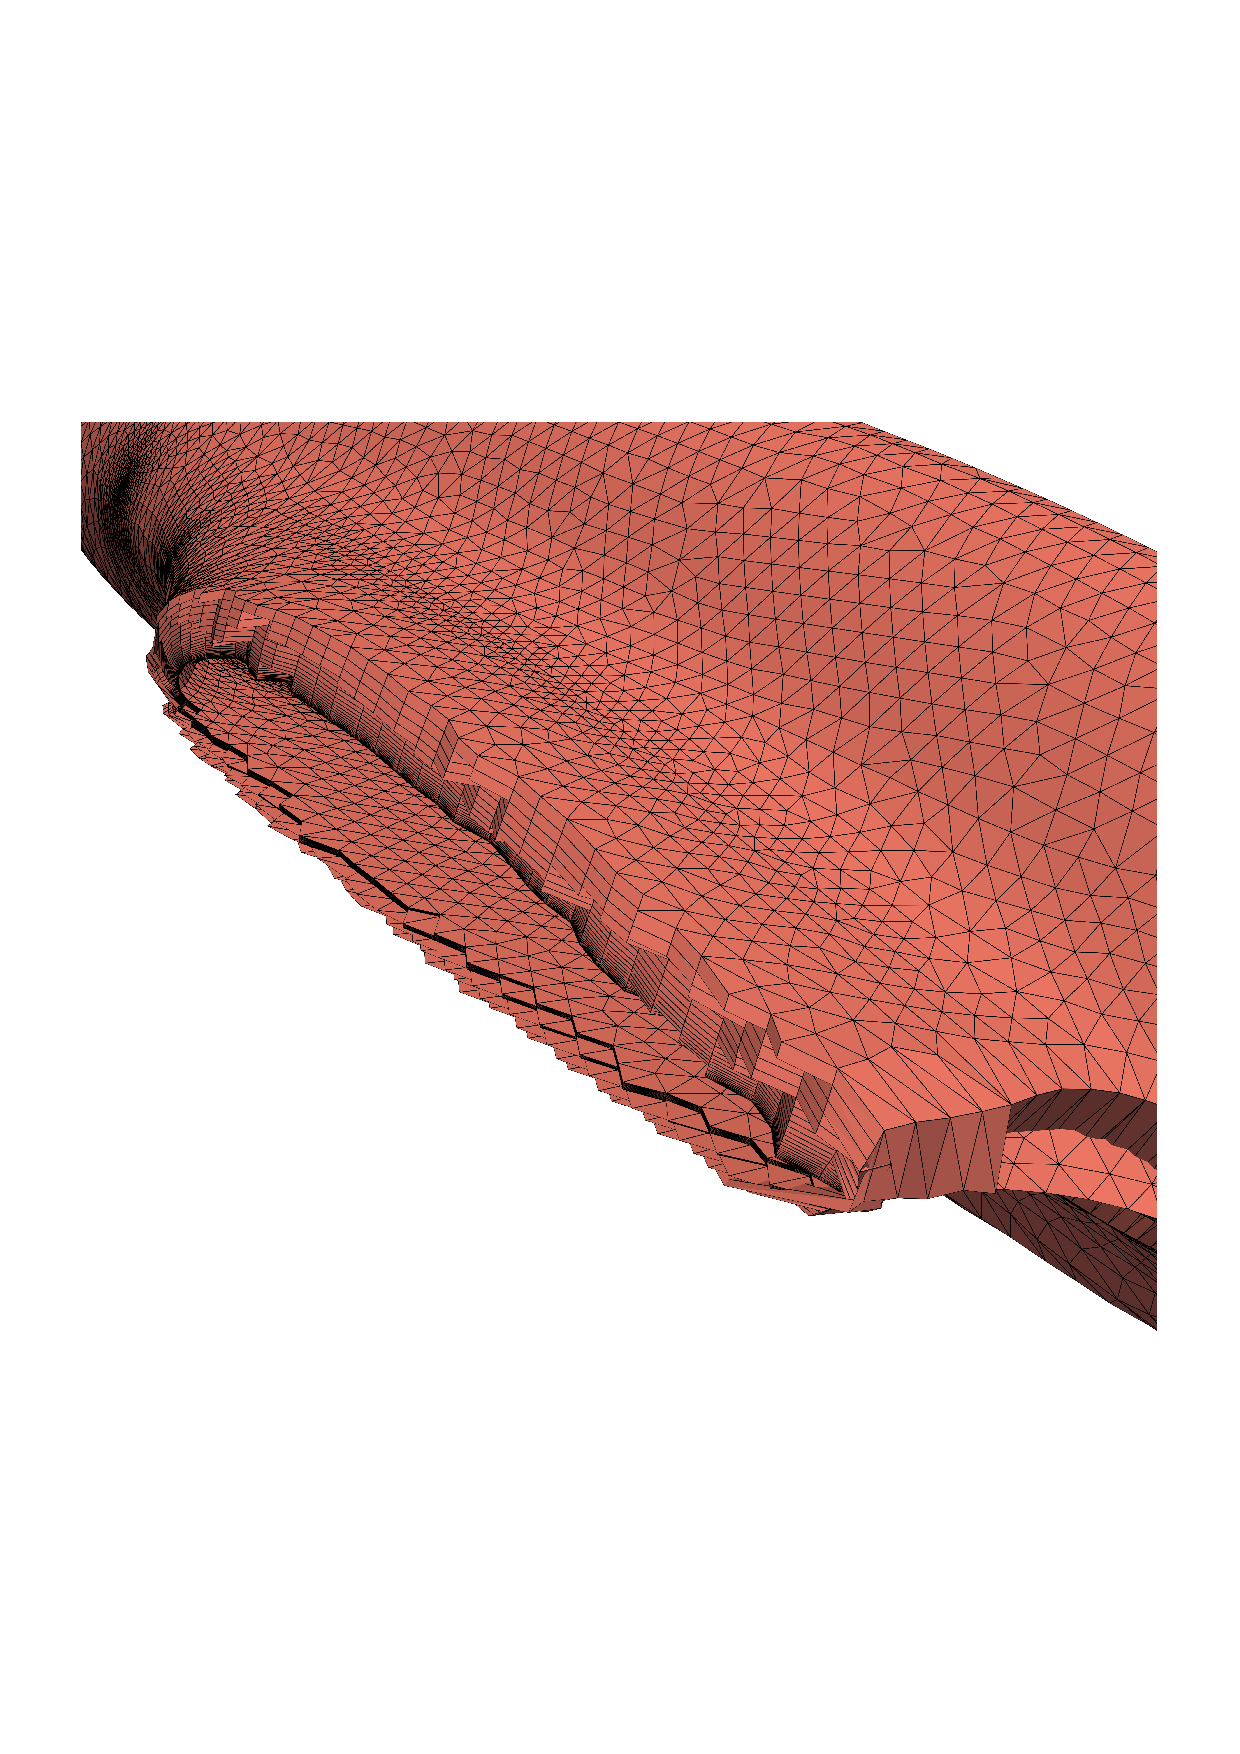
\includegraphics[width=\textwidth]{figs/6new/pl002_norm_big1.pdf}
        \caption{Unit Norm Penalty}
        \label{fig:angleloss1}
    \end{subfigure}
    \hfill
    \begin{subfigure}[b]{0.31\textwidth}
        \centering
        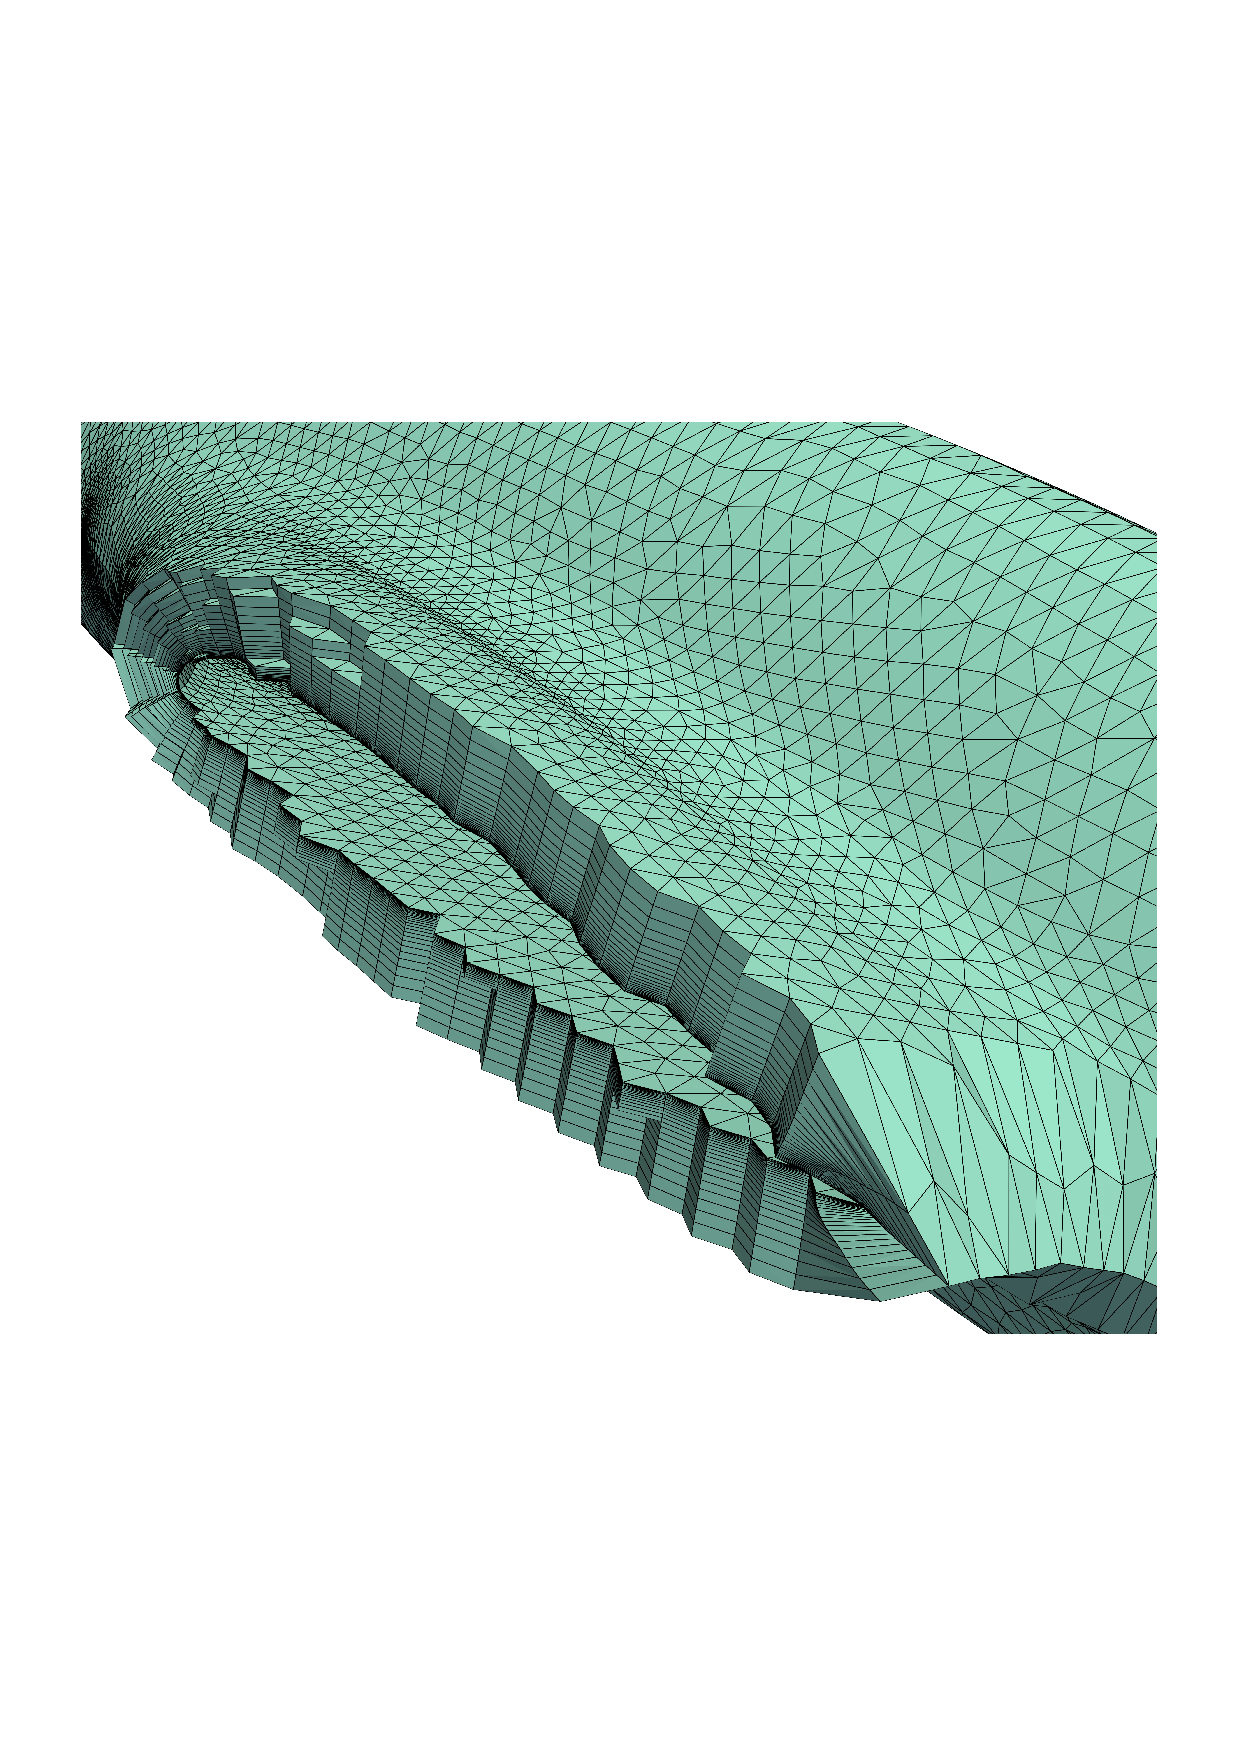
\includegraphics[width=\textwidth]{figs/6new/pl002_base_big1.pdf}
        \caption{Cosine Similarity Loss}
        \label{fig:angleloss2}
    \end{subfigure}
    \hfill
    \begin{subfigure}[b]{0.31\textwidth}
        \centering
        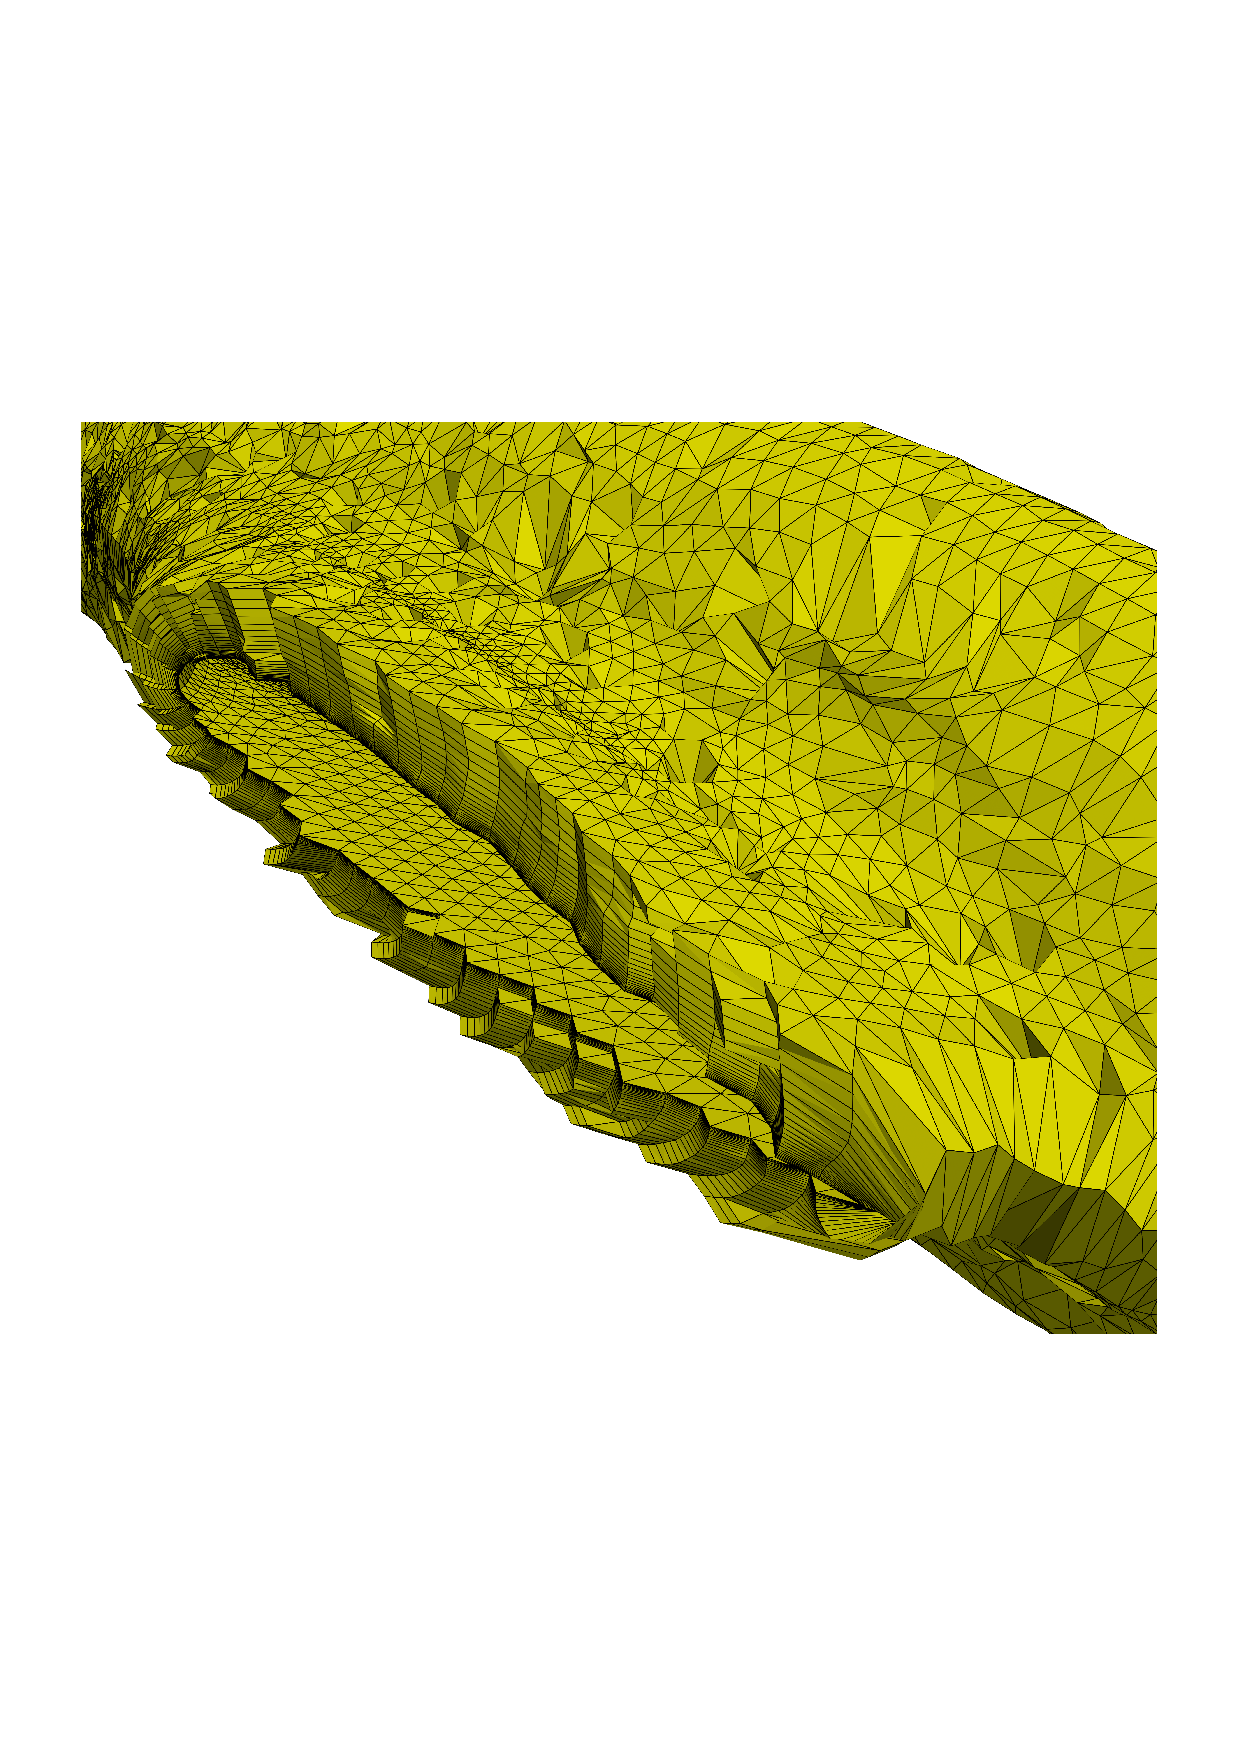
\includegraphics[width=\textwidth]{figs/6new/pl002_chord_big1.pdf}
        \caption{Squared Chord Length Loss}
        \label{fig:angleloss3}
    \end{subfigure}

    \vspace{0.8em}

    \begin{subfigure}[t]{0.31\textwidth}
        \centering
        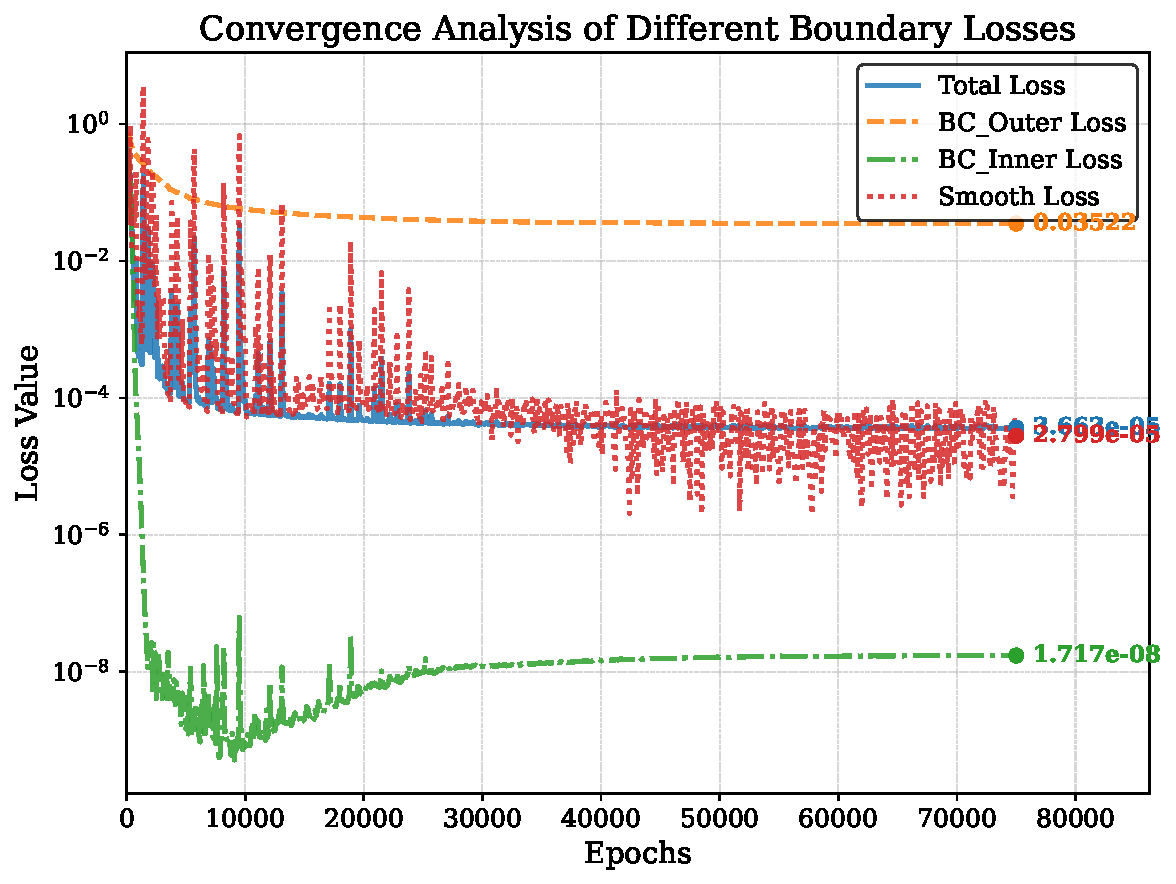
\includegraphics[width=\linewidth]{figs/6new/loss_curve_norm.pdf}
        \caption{Convergence with unit-norm penalty}
        \label{fig:losscurve1}
    \end{subfigure}
    \hfill
    \begin{subfigure}[t]{0.31\textwidth}
        \centering
        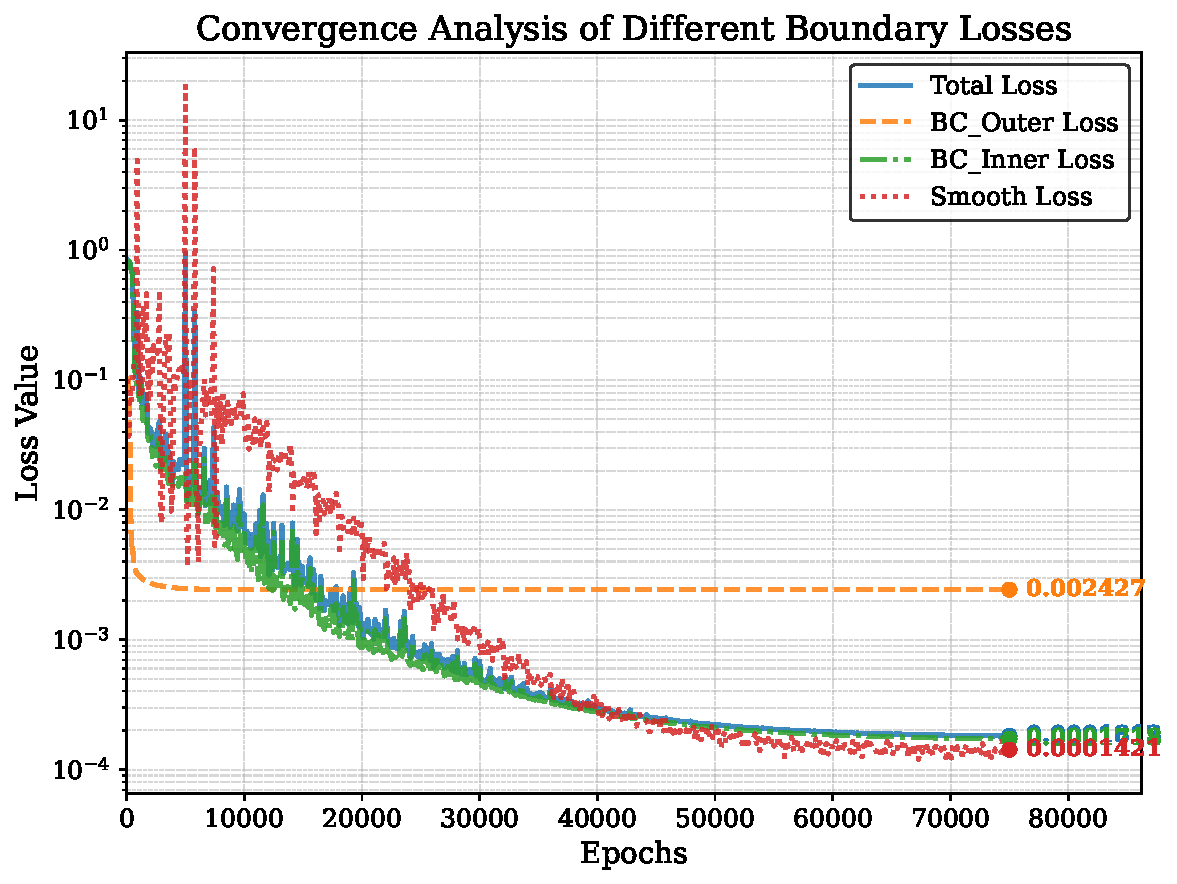
\includegraphics[width=\linewidth]{figs/6new/loss_curve_base.pdf}
        \caption{Convergence with boundary cosine loss}
        \label{fig:losscurve2}
    \end{subfigure}
    \hfill
    \begin{subfigure}[t]{0.31\textwidth}
        \centering
        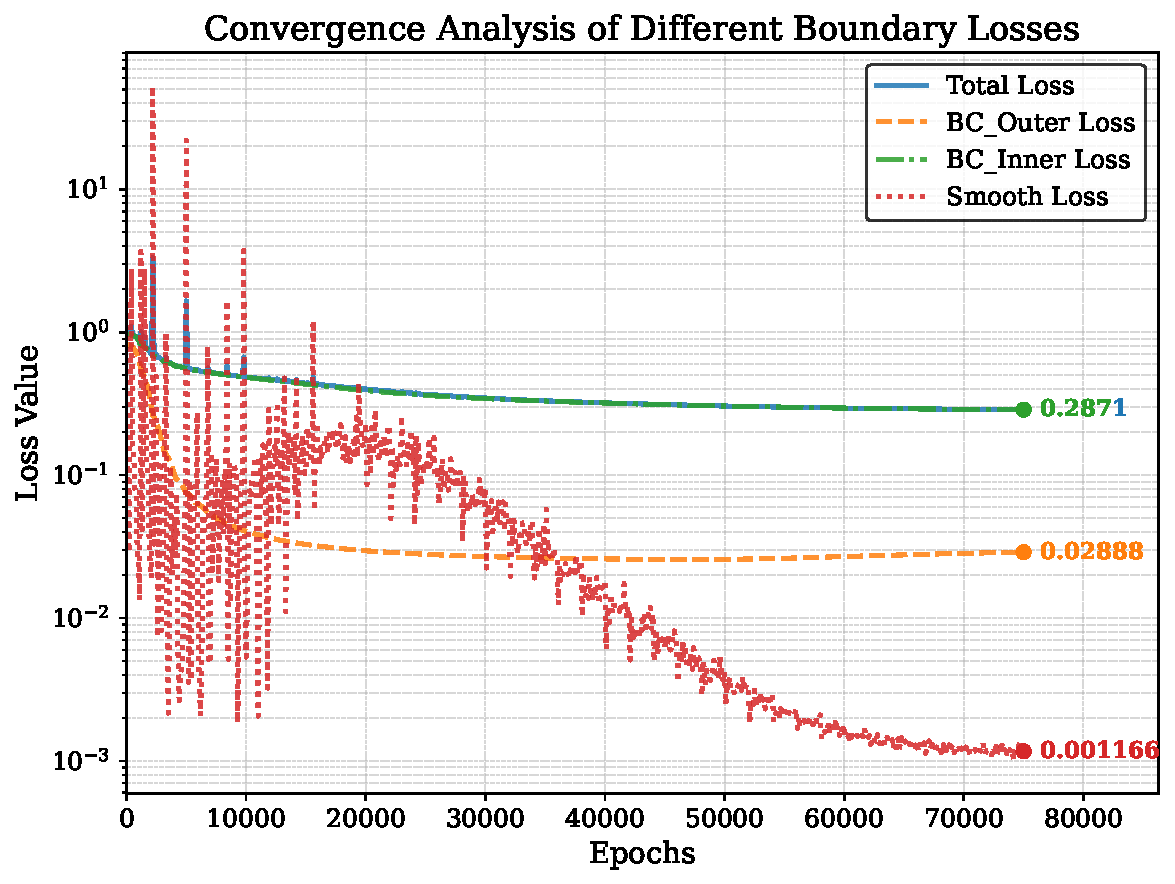
\includegraphics[width=\linewidth]{figs/6new/loss_curve_chord.pdf}
        \caption{Convergence with squared chord-length loss}
        \label{fig:losscurve3}
    \end{subfigure}

    \caption{Qualitative mesh comparison and convergence behavior under different boundary-direction loss functions}
    \label{fig:angleloss_losscurve}
\end{figure*}

The first baseline is a unit-norm penalty, which constrains only the magnitude of the supervised direction:
\begin{equation}
    \mathcal{L}_{norm}
    =
    \frac{1}{N_b}
    \sum_{i=1}^{N_b}
    \left(
    \|\mathbf{q}_i\|_2-1
    \right)^2 .
\end{equation}
The corresponding mesh and convergence behavior are shown in Fig. \ref{fig:angleloss1} and Fig. \ref{fig:losscurve1}, respectively. This formulation encourages the supervised directions to have unit magnitude, but no explicit constraint is imposed on their orientation. As a result, although the inner-boundary loss quickly decreases to a very small value, the outer-boundary loss remains at a relatively high level during training. This imbalance is reflected in the generated mesh: on the wing cross-section, the boundary-layer thickness on the upper surface advances in a relatively normal manner, whereas the lower-surface boundary layer becomes obviously too thin. In addition, discontinuities of the boundary-layer structure can be observed near the wing trailing edge, where local layers are interrupted or misaligned.
These results indicate that constraining only the vector magnitude is insufficient to guarantee continuous and directionally consistent boundary-layer growth over complex aerodynamic geometries.

The second baseline is a squared chord-length loss, which measures the Euclidean discrepancy between the supervised direction and the target direction:
\begin{equation}
    \mathcal{L}_{chord}
    =
    \frac{1}{N_b}
    \sum_{i=1}^{N_b}
    \left\|
    \mathbf{q}_i-\mathbf{n}_i
    \right\|_2^2 .
\end{equation}
As shown in Fig. \ref{fig:angleloss3} and Fig. \ref{fig:losscurve3}, this loss introduces directional information, but magnitude and angular errors are coupled in this formulation, and the optimization does not isolate orientation errors as explicitly as the cosine loss. Although the generated mesh exhibits a certain degree of directional constraint, the surface contains pronounced local undulations, together with visible distortions of the triangular boundary-layer mesh. On the wing cross-section, the boundary-layer advancing direction also shows a tendency to bend toward one side, suggesting that local directional errors are accumulated during the layer-by-layer extrusion process. These observations indicate that the squared chord-length loss contains useful directional information, but it is less direct than the cosine loss in controlling angular consistency over complex curved surfaces.

To impose the angular constraint more directly, the proposed method adopts a boundary cosine loss defined on the same supervised directions:
\begin{equation}
    \mathcal{L}_{cos}
    =
    \frac{1}{N_b}
    \sum_{i=1}^{N_b}
    \left(
    1-
    \frac{
    \mathbf{q}_i\cdot\mathbf{n}_i
    }{
    \|\mathbf{q}_i\|_2\|\mathbf{n}_i\|_2+\epsilon
    }
    \right).
\end{equation}
The improvement obtained with this formulation is shown in Fig. \ref{fig:angleloss2}, with its corresponding convergence history reported in Fig. \ref{fig:losscurve2}. This loss explicitly penalizes angular misalignment between the supervised direction and the target boundary normal, leading to a more stable and coherent result. The generated prismatic layers follow the local surface orientation more consistently, and the layer-wise extrusion remains better organized along the curved boundary. Compared with the other two loss formulations, the cosine loss maintains a more reasonable boundary-layer thickness distribution on both the upper and lower surfaces of the wing cross-section, while preserving better layer continuity near geometrically sensitive regions such as the trailing edge.
The convergence curve also shows a more balanced optimization process: the total loss, inner-boundary loss, and smoothness loss decrease steadily, while the outer-boundary loss remains substantially lower than in the unit-norm case.
This behavior confirms that the cosine formulation provides direct and effective angular supervision for the predicted vector field.

Overall, the visual comparison and convergence behavior demonstrate that the boundary cosine loss is better suited to this task than the two baseline formulations. By directly penalizing angular misalignment, it provides stronger directional supervision, reduces the accumulation of local growth-direction errors, and produces a more regular and continuous prismatic boundary-layer mesh around complex curved geometry.

% \subsubsection{\label{sec:level3-2}Impacts of PDE loss}

% \begin{figure}[htbp]
%     \centering
%     \begin{subfigure}[b]{0.23\textwidth}
%         \centering
%         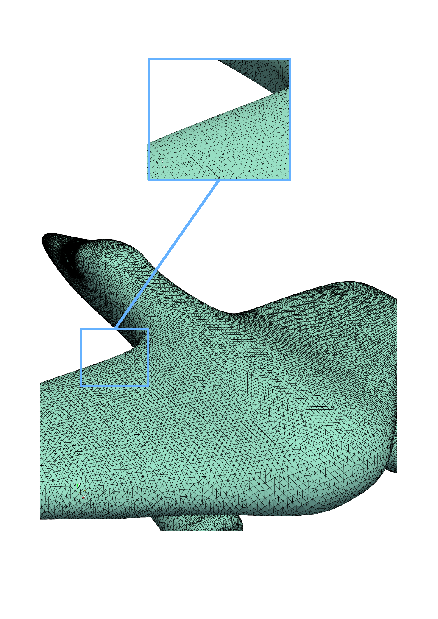
\includegraphics[width=\textwidth]{figs/6new/smoothloss1.pdf}
%         \caption{With Laplacian smoothing, \(\lambda_{\mathrm{lap}}=5 \times 10^{-2}\)}
%         \label{fig:smooth1}
%     \end{subfigure}
%     \hfill
%     \begin{subfigure}[b]{0.23\textwidth}
%         \centering
%         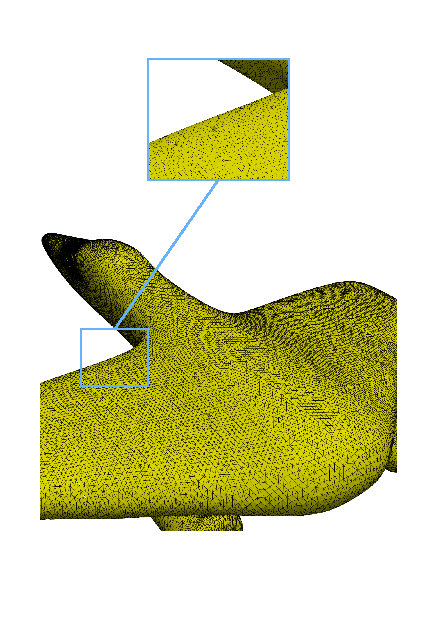
\includegraphics[width=\textwidth]{figs/6new/smoothloss2.pdf}
%         \caption{Without Laplacian smoothing, \(\lambda_{\mathrm{lap}}=0\)}
%         \label{fig:smooth2}
%     \end{subfigure}
%     \caption{Effect of the Laplacian smoothing loss on boundary-layer mesh quality. The zoomed regions show that the Laplacian smoothing term improves the spatial regularity of the predicted growth-direction field and reduces localized mesh artifacts in high-curvature regions.}
%     \label{fig:smooth}
% \end{figure}

% \begin{table*}[htbp]
%     \centering
%     \caption{Quantitative comparison of mesh quality with and without PDE loss regularization}
%     \label{tab:mesh_quality_pdeloss}
%     \renewcommand{\arraystretch}{1.2}
%     \begin{tabular}{l *{12}{c}}
%         \toprule
%         \multirow{3}{*}{\textbf{Models}} 
%         & \multicolumn{6}{c}{\textbf{\(\lambda=0\)}} 
%         & \multicolumn{6}{c}{\textbf{\(\lambda=5 \times 10^{-2}\)}} \\
%         \cmidrule(lr){2-7} \cmidrule(lr){8-13}
%         & \multicolumn{3}{c}{\textbf{Orthogonal Quality}} 
%         & \multicolumn{3}{c}{\textbf{Equiangle Skewness}} 
%         & \multicolumn{3}{c}{\textbf{Orthogonal Quality}} 
%         & \multicolumn{3}{c}{\textbf{Equiangle Skewness}} \\
%         \cmidrule(lr){2-4} \cmidrule(lr){5-7} 
%         \cmidrule(lr){8-10} \cmidrule(lr){11-13}
%         & \textbf{max} & \textbf{min} & \textbf{ave} 
%         & \textbf{max} & \textbf{min} & \textbf{ave} 
%         & \textbf{max} & \textbf{min} & \textbf{ave} 
%         & \textbf{max} & \textbf{min} & \textbf{ave} \\
%         \midrule
%         model1  & 0.9714 & 0.9512 & 0.9612 & 0.2319 & 0.3120 & 0.2712 & 0.9718 & 0.9500 & 0.9620 & 0.2319 & 0.3100 & 0.2700 \\
%         model2  & 0.9142 & 0.8900 & 0.9021 & 0.3360 & 0.4200 & 0.3780 & 0.9141 & 0.8880 & 0.9010 & 0.3360 & 0.4180 & 0.3770 \\
%         model3  & 0.9866 & 0.9700 & 0.9783 & 0.1670 & 0.2500 & 0.2085 & 0.9870 & 0.9710 & 0.9790 & 0.1662 & 0.2480 & 0.2071 \\
%         \bottomrule
%     \end{tabular}
% \end{table*}


% \begin{table}[hbt]
%     \centering
%     \caption{Comparison of Average mesh quality between different layers for the model3}
%     \label{tab:ablation_study:pdeloss}
%     \renewcommand{\arraystretch}{1.2} % 稍微拉宽行距，显得不拥挤
%     \begin{tabular}{l c c c c}
%         \toprule
%         \multirow{2}{*}{\textbf{layer}} & \multicolumn{2}{c}{\textbf{Orthogonal Quality}} & \multicolumn{2}{c}{\textbf{Equiangle Skewness}}\\
%         \cmidrule(lr){2-3} \cmidrule(lr){4-5}
%         & $\lambda=0$ & $\lambda=5^{-2}$ & $\lambda=0$ & $\lambda=5^{-2}$\\
%         \midrule
%         15    &0.8612&0.8612&0.2688&0.2688\\
%         20    &0.8614&0.8617&0.2693&0.2687\\
%         25    &0.8609&0.8625&0.2713&0.2686\\
%         30    &0.8599&0.8632&0.2747&0.2693\\
%         35    &0.8579&0.8632&0.2810&0.2729\\
%         \bottomrule
%     \end{tabular}
% \end{table}
\subsubsection{\label{sec:level3-2}Impacts of Laplacian Smoothing Loss}

\begin{figure}[htbp]
    \centering
    \begin{subfigure}[b]{0.23\textwidth}
        \centering
        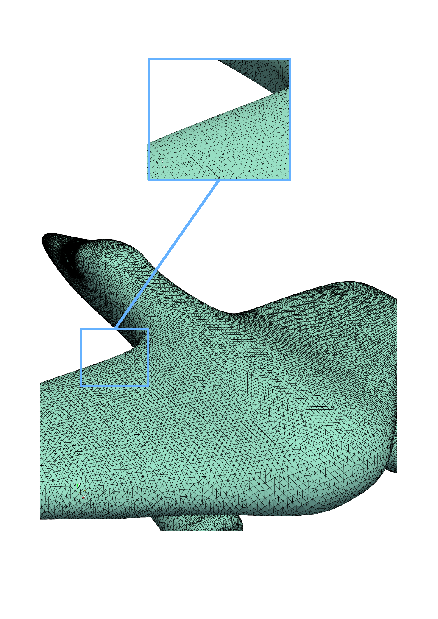
\includegraphics[width=\textwidth]{figs/6new/smoothloss1.pdf}
        \caption{With Laplacian smoothing, \(\lambda_{\mathrm{s}}=5 \times 10^{-2}\)}
        \label{fig:smooth1}
    \end{subfigure}
    \hfill
    \begin{subfigure}[b]{0.23\textwidth}
        \centering
        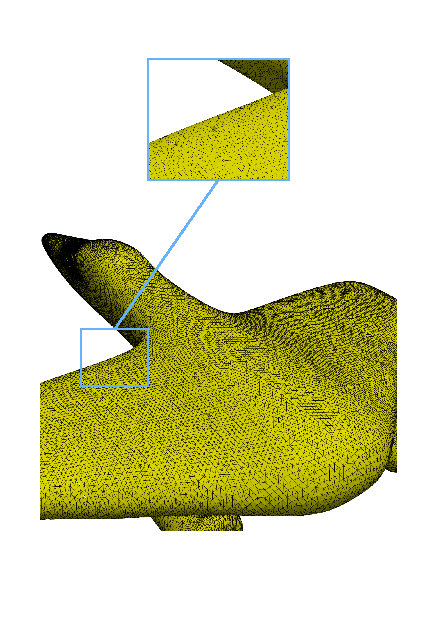
\includegraphics[width=\textwidth]{figs/6new/smoothloss2.pdf}
        \caption{Without Laplacian smoothing, \(\lambda_{\mathrm{s}}=0\)}
        \label{fig:smooth2}
    \end{subfigure}
    \caption{Effect of the Laplacian smoothing loss on boundary-layer mesh quality. The zoomed regions show that the Laplacian smoothing term improves the spatial regularity of the predicted growth-direction field and reduces localized mesh artifacts in high-curvature regions.}
    \label{fig:smooth}
\end{figure}

\begin{table*}[htbp]
    \centering
    \caption{Quantitative comparison of mesh quality with and without Laplacian smoothing regularization across different models.}
    \label{tab:mesh_quality_pdeloss}
    \renewcommand{\arraystretch}{1.2}
    \begin{tabular}{l *{12}{c}}
        \toprule
        \multirow{3}{*}{\textbf{Models}} 
        & \multicolumn{6}{c}{\textbf{\(\lambda=0\)}} 
        & \multicolumn{6}{c}{\textbf{\(\lambda=5 \times 10^{-2}\)}} \\
        \cmidrule(lr){2-7} \cmidrule(lr){8-13}
        & \multicolumn{3}{c}{\textbf{Orthogonal Quality}} 
        & \multicolumn{3}{c}{\textbf{Equiangle Skewness}} 
        & \multicolumn{3}{c}{\textbf{Orthogonal Quality}} 
        & \multicolumn{3}{c}{\textbf{Equiangle Skewness}} \\
        \cmidrule(lr){2-4} \cmidrule(lr){5-7} 
        \cmidrule(lr){8-10} \cmidrule(lr){11-13}
        & \textbf{Max.} & \textbf{Min.} & \textbf{Ave.} 
        & \textbf{Max.} & \textbf{Min.} & \textbf{Ave.} 
        & \textbf{Max.} & \textbf{Min.} & \textbf{Ave.} 
        & \textbf{Max.} & \textbf{Min.} & \textbf{Ave.} \\
        \midrule
        model1  & 0.9714 & 0.9512 & 0.9612 & 0.2319 & 0.3120 & 0.2712 & 0.9718 & 0.9500 & 0.9620 & 0.2319 & 0.3100 & 0.2700 \\
        model2  & 0.9142 & 0.8900 & 0.9021 & 0.3360 & 0.4200 & 0.3780 & 0.9141 & 0.8880 & 0.9010 & 0.3360 & 0.4180 & 0.3770 \\
        model3  & 0.9866 & 0.9700 & 0.9783 & 0.1670 & 0.2500 & 0.2085 & 0.9870 & 0.9710 & 0.9790 & 0.1662 & 0.2480 & 0.2071 \\
        \bottomrule
    \end{tabular}
\end{table*}

To validate the role of the Laplacian smoothing loss in maintaining the stability of the domain vector field, we conducted an ablation study across three distinct geometric models. We compared the visual results and quantitative mesh quality metrics of models optimized with Laplacian smoothing regularization \((\lambda_{\mathrm{s}} = 5 \times 10^{-2})\) against a baseline where this term was removed \((\lambda_{\mathrm{s}} = 0)\).

As shown in Fig. \ref{fig:smooth}, the model trained with Laplacian smoothing produces a smoother surface mesh. In the zoomed region, the triangular elements exhibit more continuous transitions, without obvious localized depressions or irregular surface fluctuations. This indicates that the Laplacian smoothing term improves the spatial continuity of the predicted growth-direction field and thereby enhances the local boundary-layer mesh quality near high-curvature regions. In contrast, when the Laplacian smoothing term is removed, the overall geometric profile is still preserved, but fine-scale surface fluctuations and local irregularities become more visible. The zoomed region further shows that, without an explicit smoothness constraint, localized high-frequency perturbations in the predicted vector field can be transferred to the boundary-layer mesh surface, leading to degraded local mesh quality.

Quantitatively, as reported in Table \ref{tab:mesh_quality_pdeloss}, the overall mesh quality obtained with Laplacian smoothing is slightly improved compared with the baseline configuration. Across the three tested models, the average orthogonal quality remains stable or increases after applying the smoothing regularization, while the average equiangle skewness is reduced. These results indicate that the Laplacian smoothing term contributes to improved orthogonality and element-shape quality. Furthermore, we observed an important phenomenon: the performance gap between the two configurations gradually widens as the number of generated boundary layers increases.

This phenomenon is consistent with our theoretical expectation.
During the generation of the initial layers, the spatial points are in close proximity to the physical surface, where the vector field is strongly dominated by the inner-boundary loss.
This localized constraint enforces directional alignment and partially masks potential high-frequency microscopic oscillations produced by the network, thereby preserving the quality of the initial layers.
However, as the advancing front extends outward and the number of layers increases, the spatial points move farther from the surface, causing the direct constraining influence of the inner-boundary supervision to decay.
Consequently, the directional guidance for mesh growth relies increasingly on the network's generalized output field within the continuous domain.

Without the explicit spatial smoothness prior provided by the Laplacian smoothing loss, the highly sensitive multiresolution HashGrid encoder tends to produce localized high-frequency oscillations in these less-constrained deeper regions.
During the layer-by-layer numerical integration of the advancing-layer algorithm, these microscopic directional errors accumulate and are amplified, ultimately leading to degradation in deep-layer mesh quality and local surface irregularities. Conversely, the Laplacian smoothing loss enforces second-order spatial continuity across the computational domain. This compensates for the decay of the boundary supervision signal in deeper regions, suppresses localized high-frequency perturbations, and promotes more robust and continuous boundary-layer mesh growth.

\begin{table}[hbt]
    \centering
    \caption{Comparison of average mesh quality between different layers for model3.}
    \label{tab:ablation_study:pdeloss}
    \renewcommand{\arraystretch}{1.2}
    \begin{tabular}{l c c c c}
        \toprule
        \multirow{2}{*}{\textbf{Layer}} & \multicolumn{2}{c}{\textbf{Orthogonal Quality}} & \multicolumn{2}{c}{\textbf{Equiangle Skewness}}\\
        \cmidrule(lr){2-3} \cmidrule(lr){4-5}
        & $\lambda=0$ & $\lambda=5 \times 10^{-2}$ & $\lambda=0$ & $\lambda=5 \times 10^{-2}$\\
        \midrule
        15    &0.8612&0.8612&0.2688&0.2688\\
        20    &0.8614&0.8617&0.2693&0.2687\\
        25    &0.8609&0.8625&0.2713&0.2686\\
        30    &0.8599&0.8632&0.2747&0.2693\\
        35    &0.8579&0.8632&0.2810&0.2729\\
        \bottomrule
    \end{tabular}
\end{table}

\subsubsection{\label{sec:level3-3}Impacts of the Multiresolution HashGrid Encoder}

To investigate the impact of the multiresolution HashGrid encoder on complex geometric representation, we conducted a comparative study between the proposed HashGrid-encoded neural field and a conventional Multi-Layer Perceptron (MLP) baseline across three geometric models. The HashGrid-encoded neural field is referred to as the HashGrid method in the following discussion for brevity. Fig. \ref{fig:structure} presents the local mesh generation results and the corresponding equiangle-skewness maps for two representative regions of model2. For each region, the generated boundary-layer mesh and the associated quality distribution are shown for both the HashGrid and MLP methods, enabling a direct comparison of local geometric fidelity, advancing-layer stability, and mesh-quality distribution.

\begin{figure*}[t]
    \centering

    \begin{subfigure}[b]{0.23\textwidth}
        \centering
        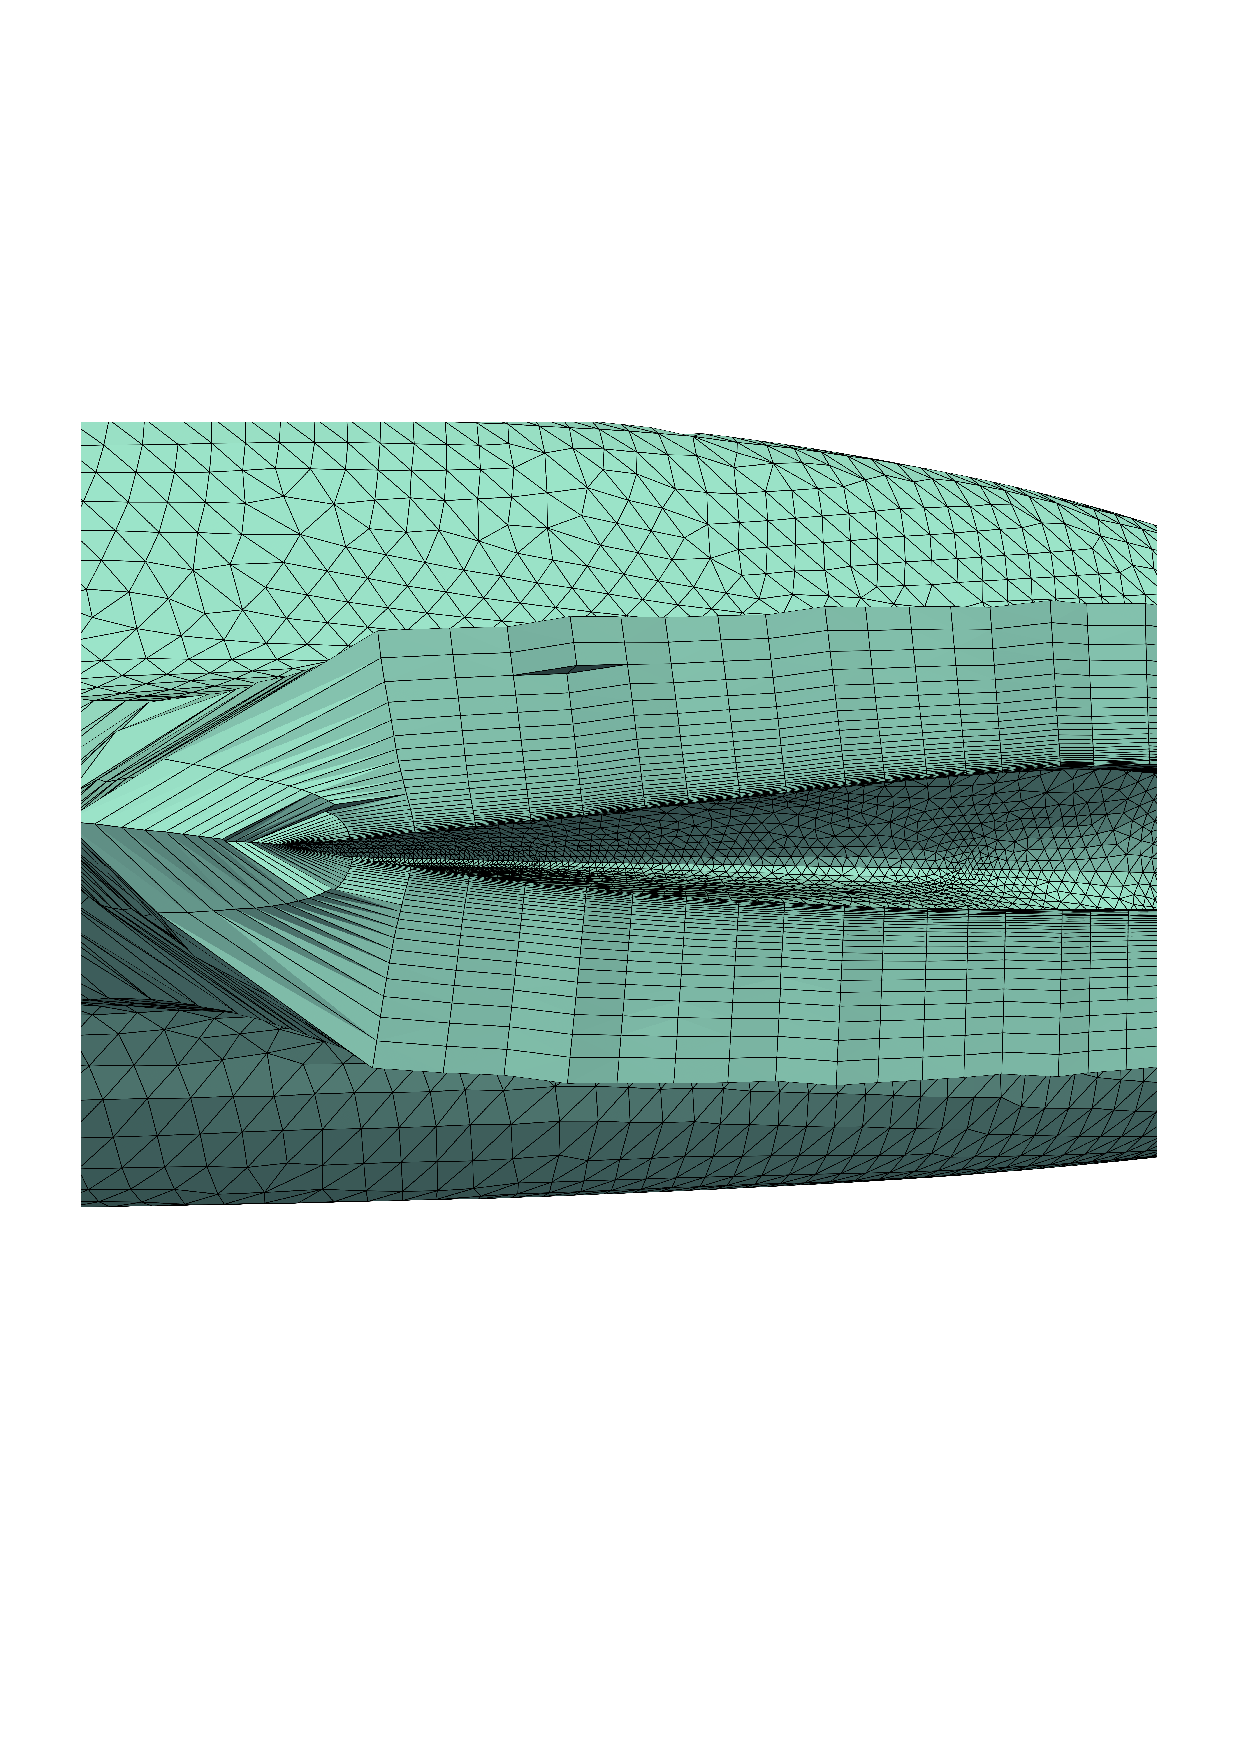
\includegraphics[width=\textwidth]{figs/6new/pl002_hash1.pdf}
        \caption{HashGrid mesh, region 1}
        \label{fig:structure1}
    \end{subfigure}
    \hfill
    \begin{subfigure}[b]{0.23\textwidth}
        \centering
        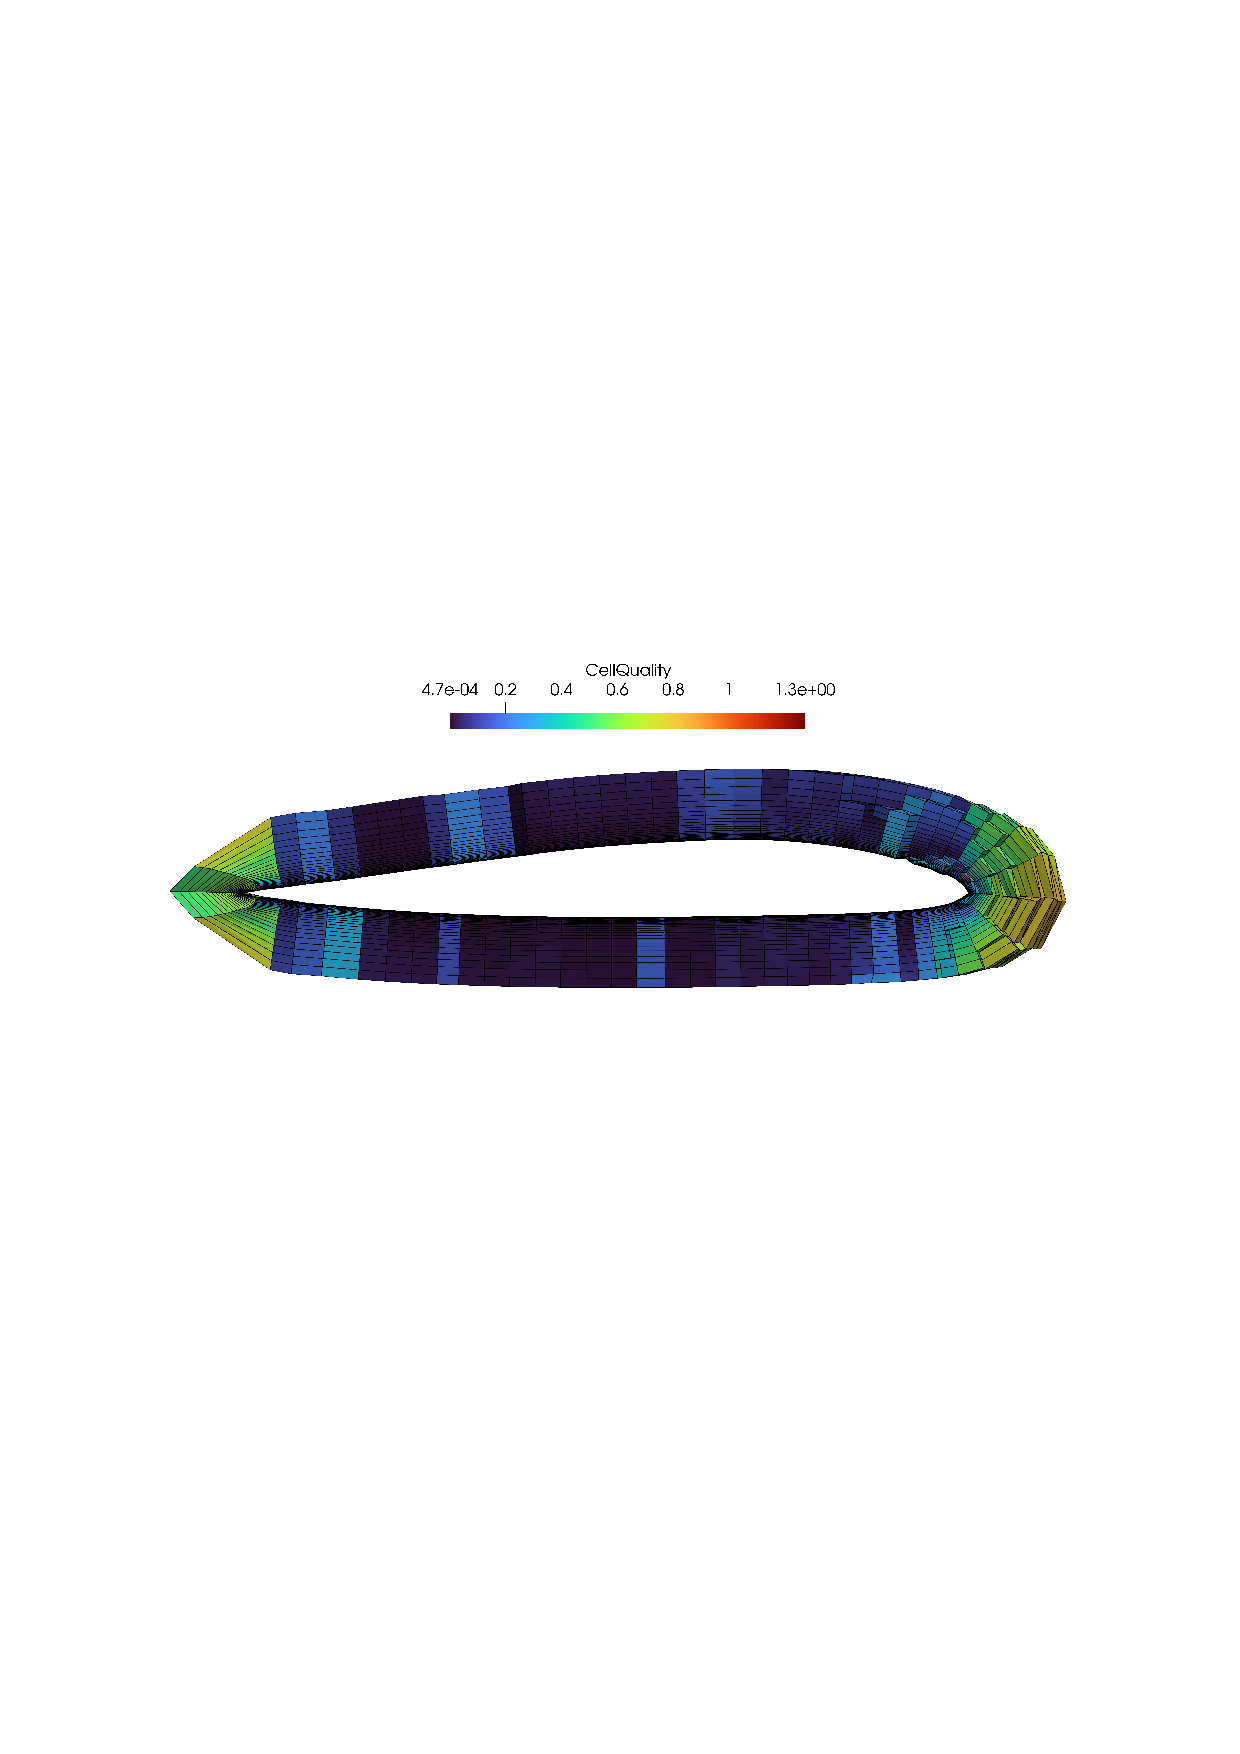
\includegraphics[width=\textwidth]{figs/6new/pl002_hash1_q.pdf}
        \caption{HashGrid equiangle-skewness map, region 1}
        \label{fig:structure2}
    \end{subfigure}
    \hfill
    \begin{subfigure}[b]{0.23\textwidth}
        \centering
        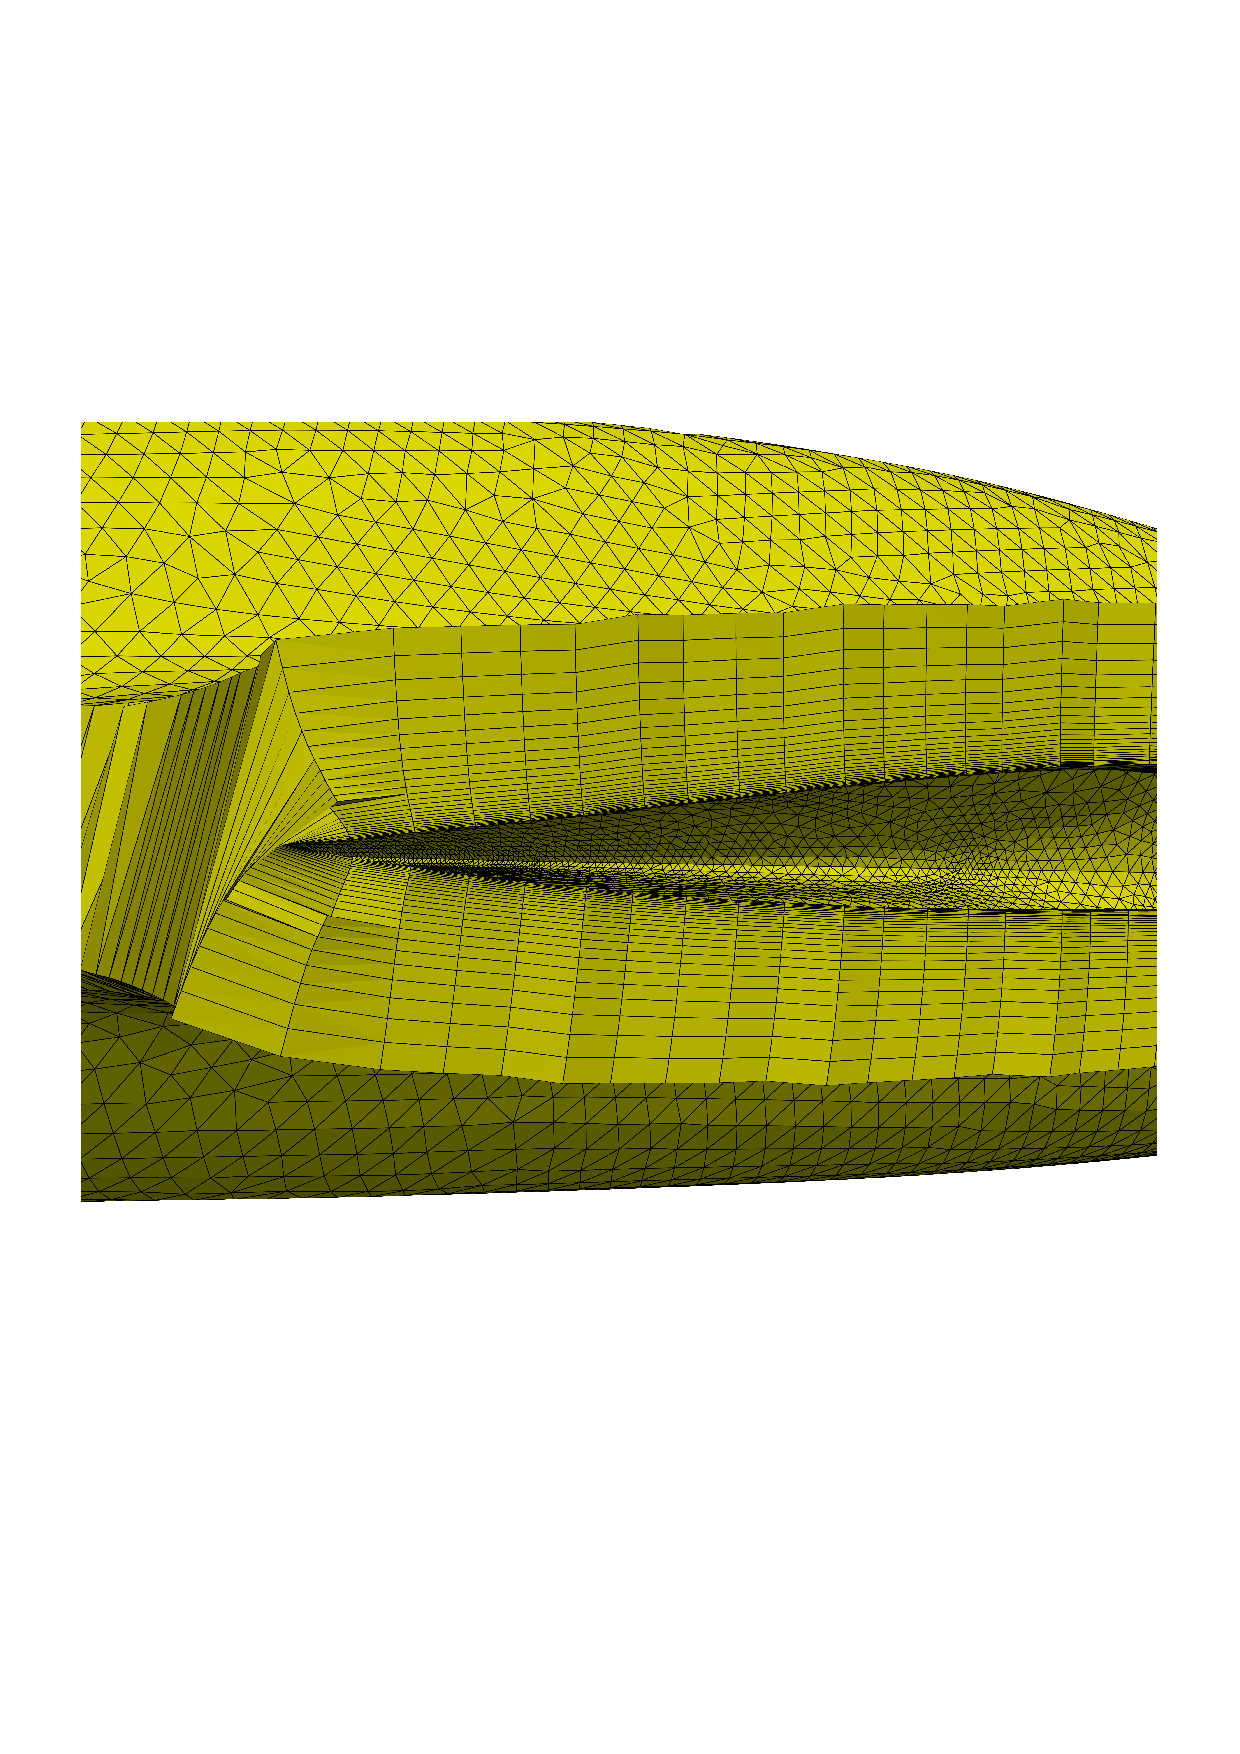
\includegraphics[width=\textwidth]{figs/6new/pl002_mlp1.pdf}
        \caption{MLP mesh, region 1}
        \label{fig:structure3}
    \end{subfigure}
    \hfill
    \begin{subfigure}[b]{0.23\textwidth}
        \centering
        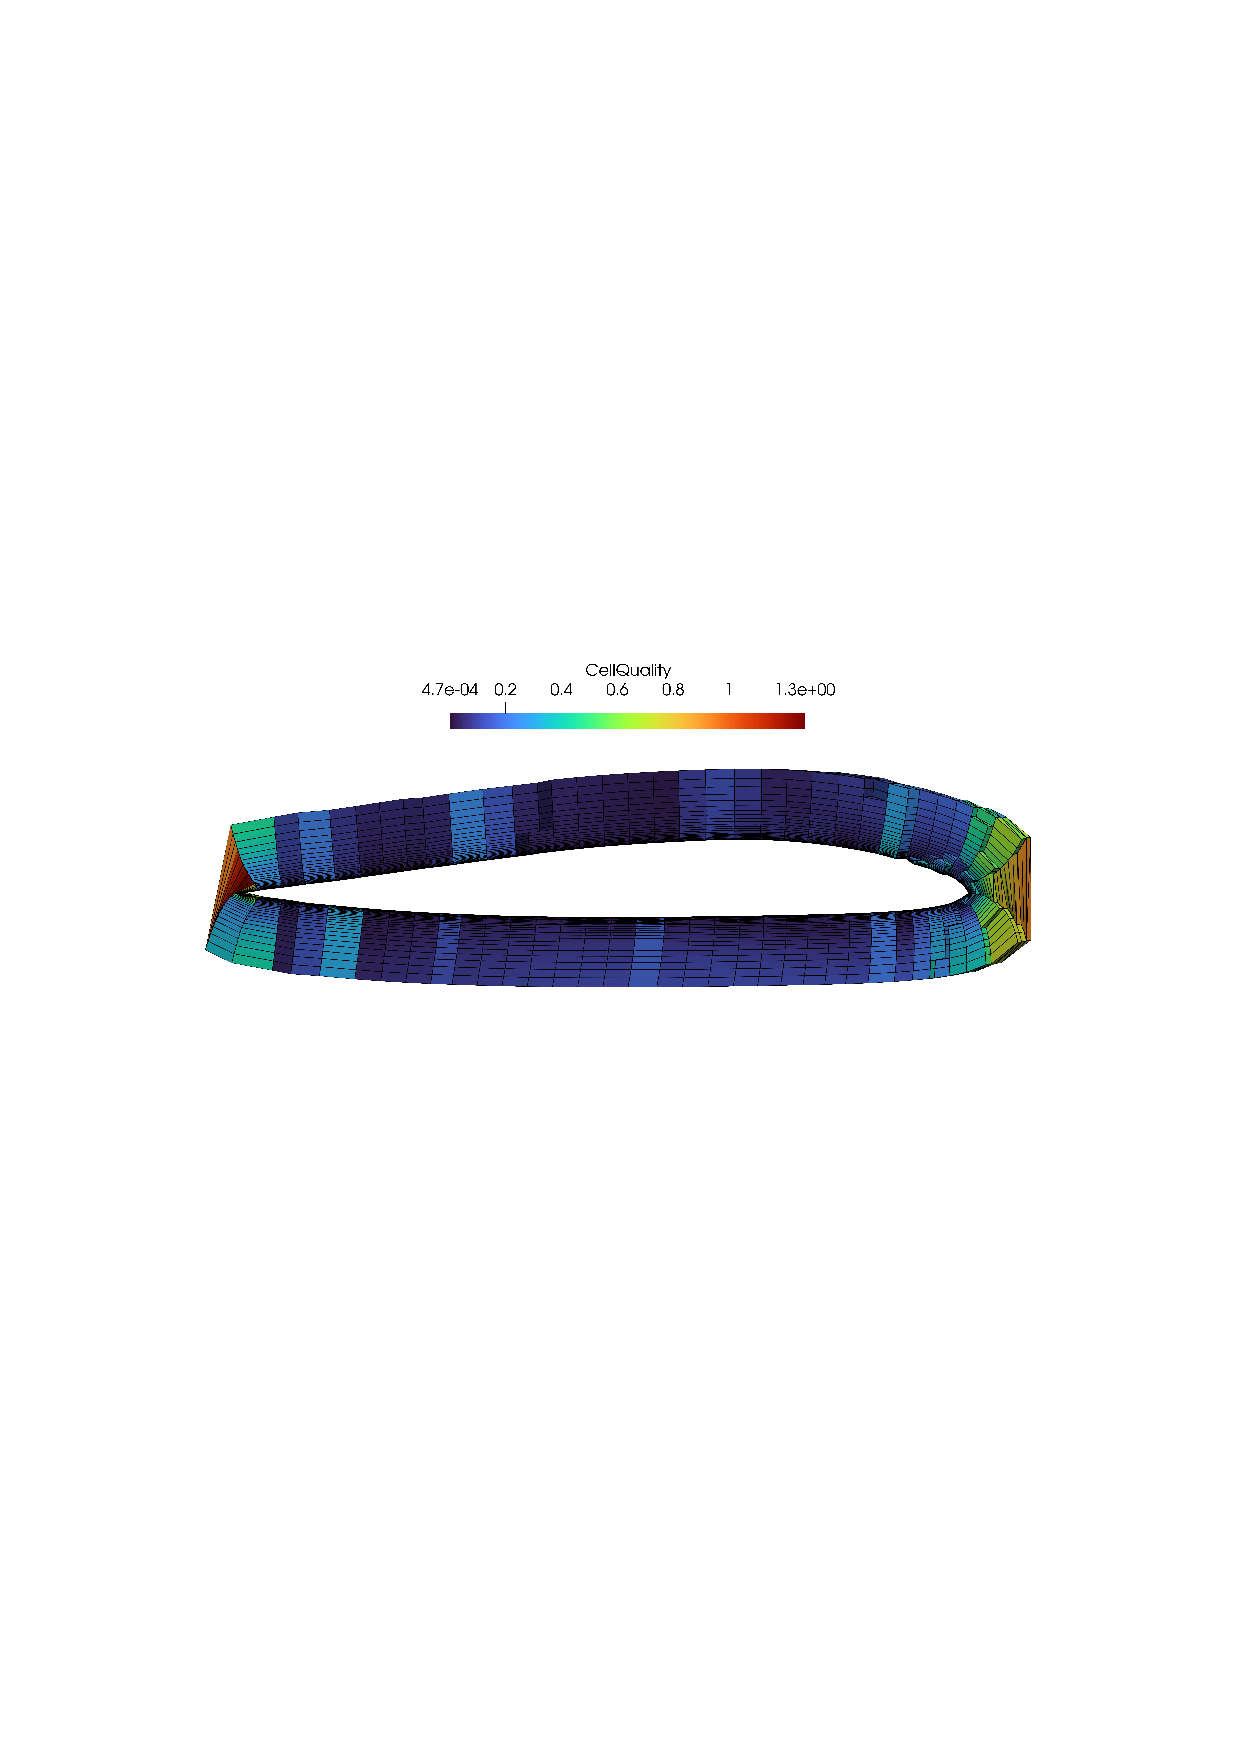
\includegraphics[width=\textwidth]{figs/6new/pl002_mlp1_q.pdf}
        \caption{MLP equiangle-skewness map, region 1}
        \label{fig:structure4}
    \end{subfigure}

    \vspace{0.8em}

    \begin{subfigure}[t]{0.23\textwidth}
        \centering
        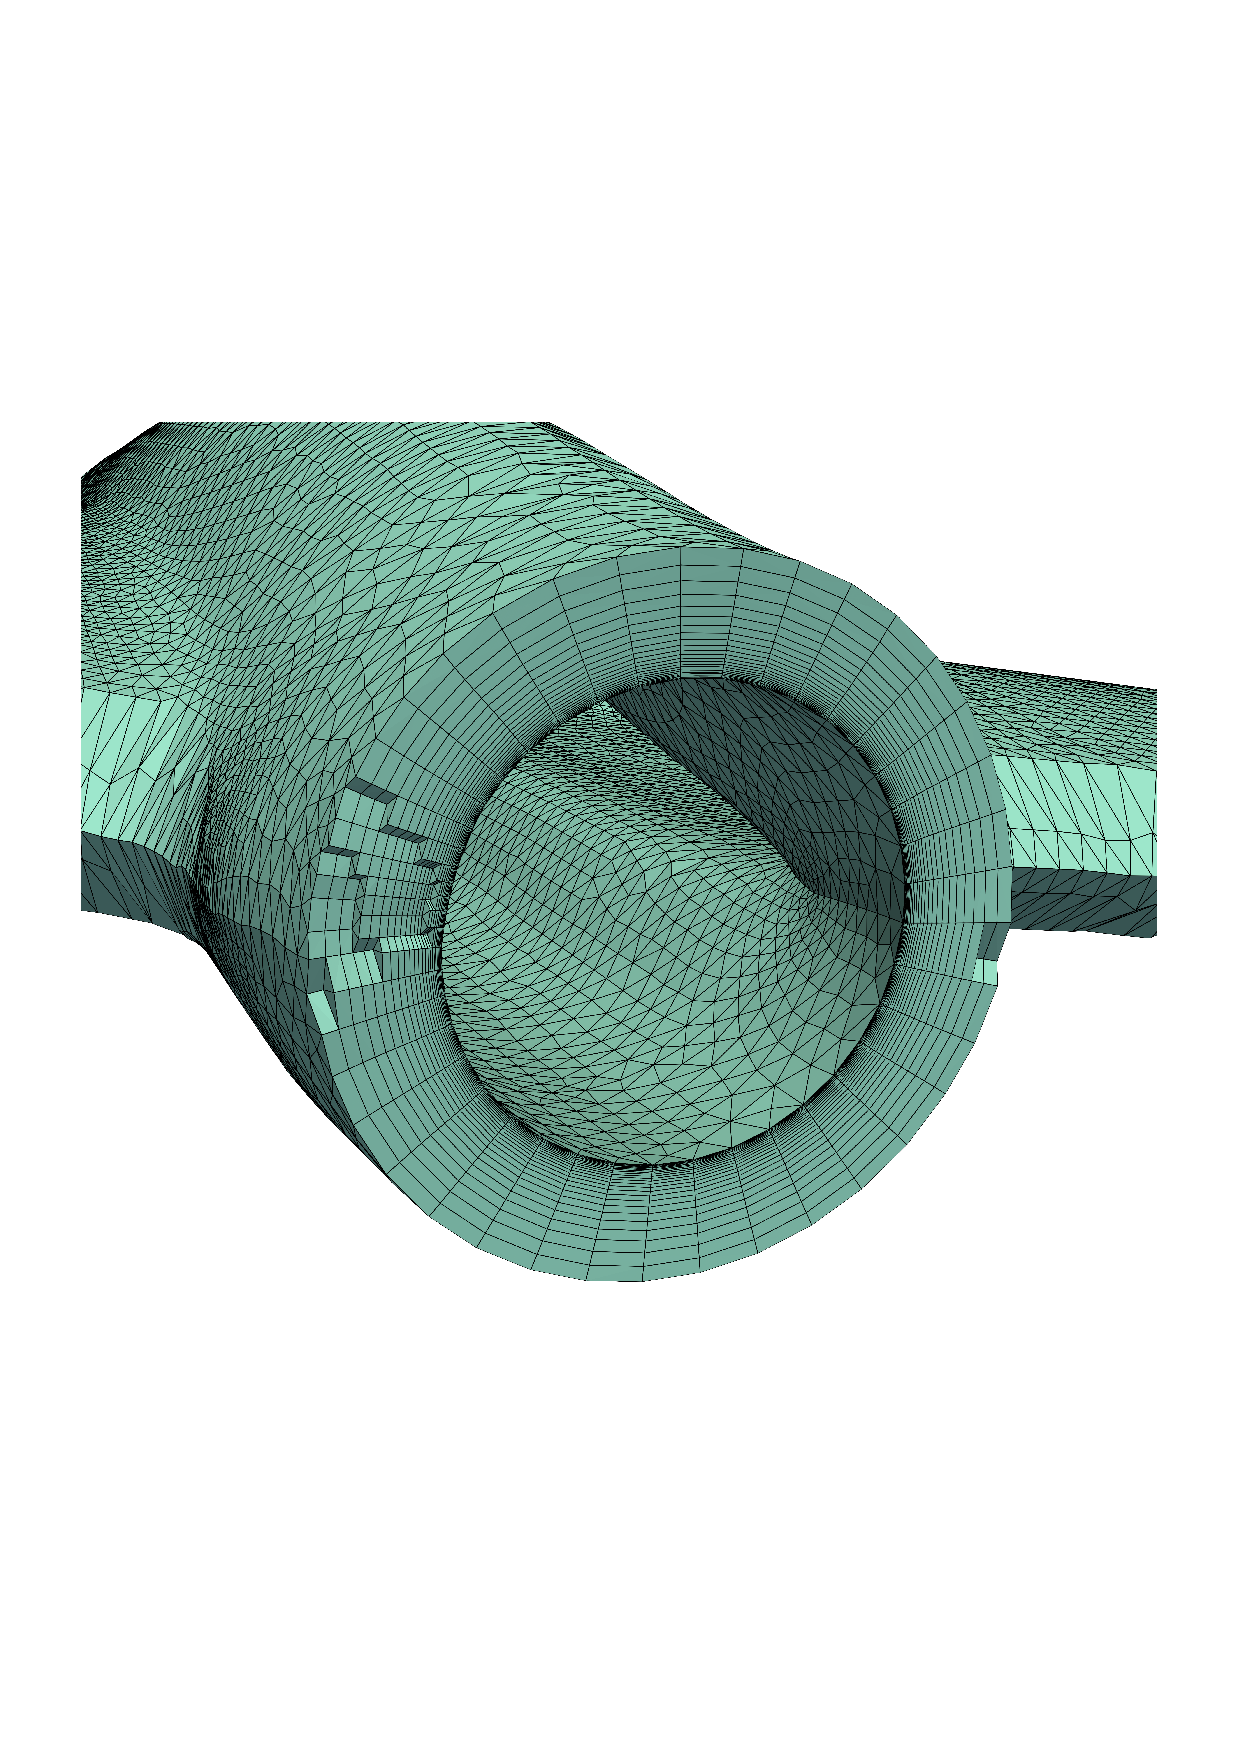
\includegraphics[width=\linewidth]{figs/6new/pl002_hash2.pdf}
        \caption{HashGrid mesh, region 2}
        \label{fig:structure5}
    \end{subfigure}
    \hfill
    \begin{subfigure}[t]{0.23\textwidth}
        \centering
        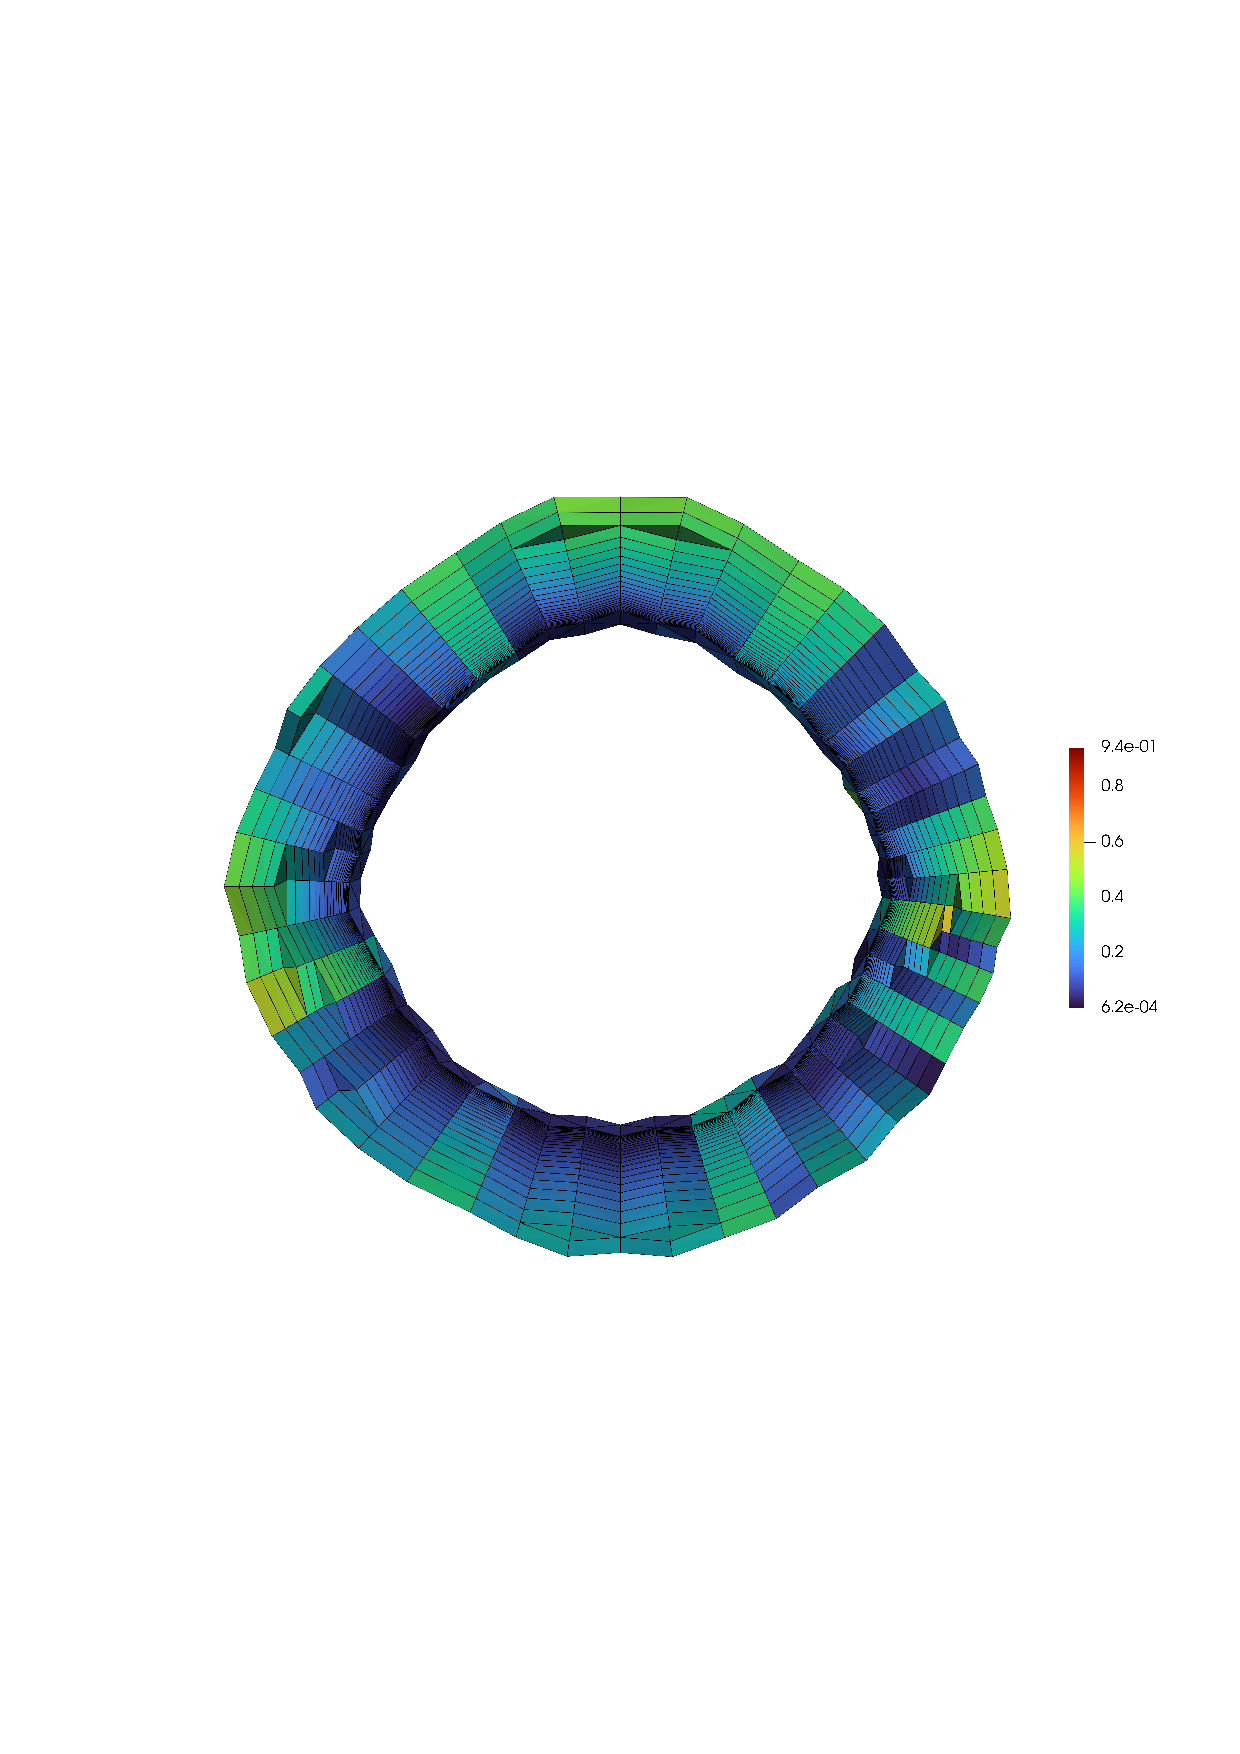
\includegraphics[width=\linewidth]{figs/6new/pl002_hash2_q.pdf}
        \caption{HashGrid equiangle-skewness map, region 2}
        \label{fig:structure6}
    \end{subfigure}
    \hfill
    \begin{subfigure}[t]{0.23\textwidth}
        \centering
        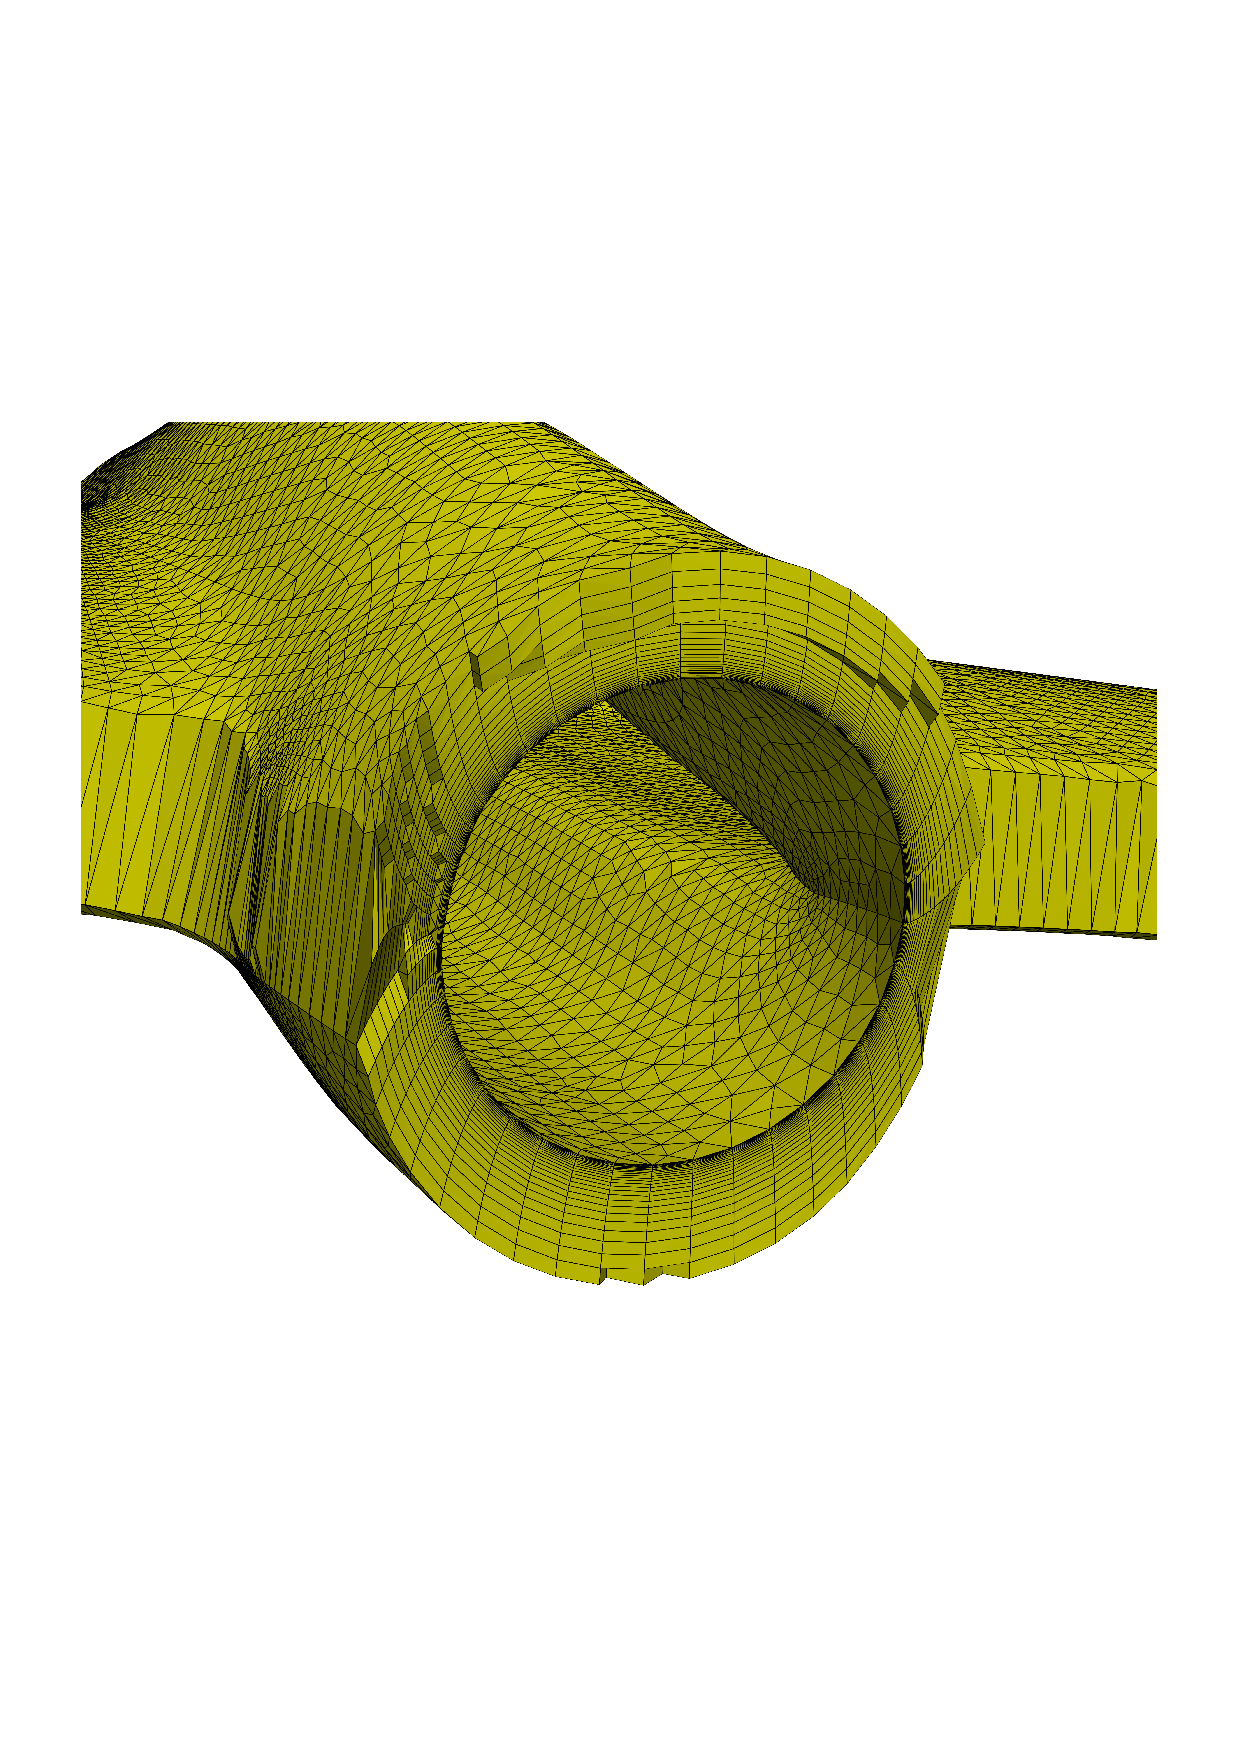
\includegraphics[width=\linewidth]{figs/6new/pl002_mlp2.pdf}
        \caption{MLP mesh, region 2}
        \label{fig:structure7}
    \end{subfigure}
    \hfill
    \begin{subfigure}[t]{0.23\textwidth}
        \centering
        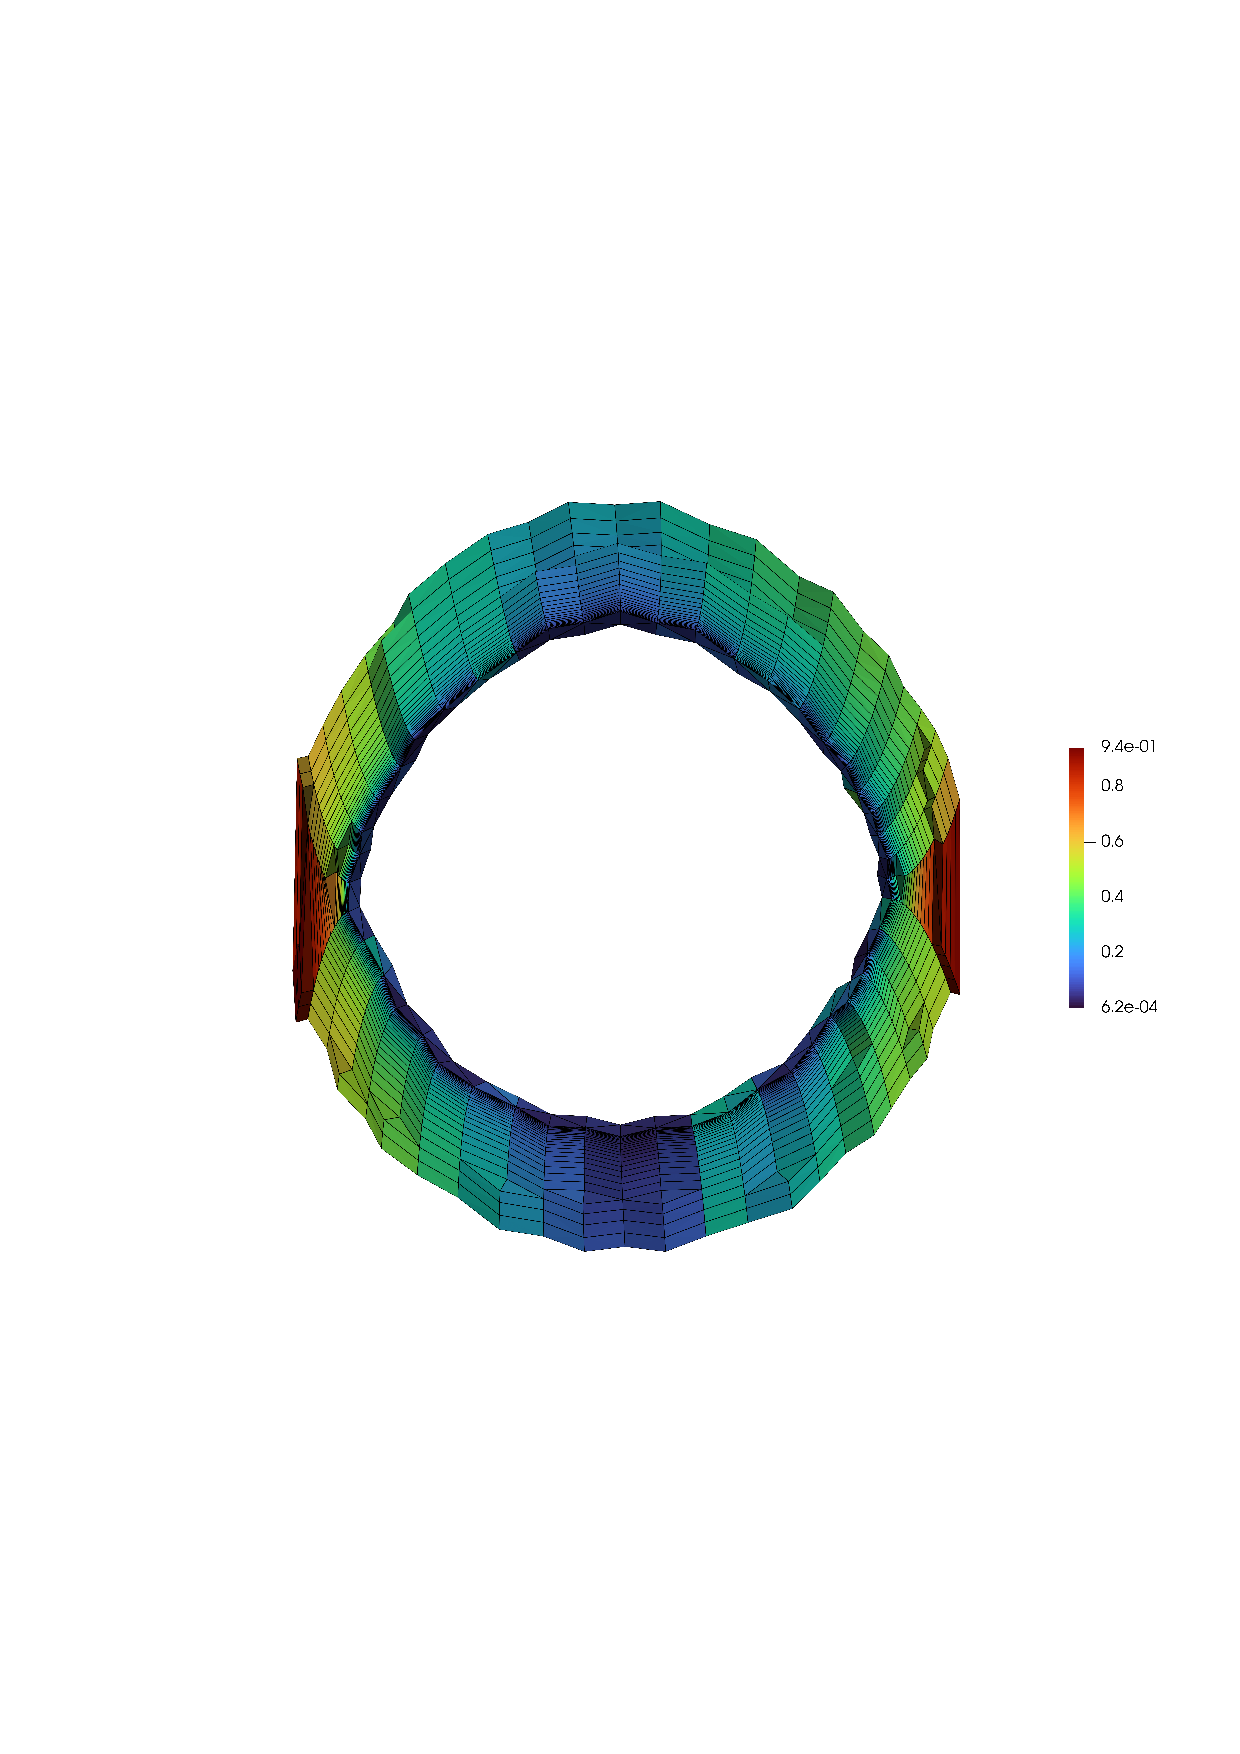
\includegraphics[width=\linewidth]{figs/6new/pl002_mlp2_q.pdf}
        \caption{MLP equiangle-skewness map, region 2}
        \label{fig:structure8}
    \end{subfigure}

    \caption{Local mesh generation and equiangle-skewness comparison between the HashGrid-encoded neural field and the MLP baseline in two representative regions of model2.}
    \label{fig:structure}
\end{figure*}

As shown in Fig. \ref{fig:structure}, the HashGrid method generates more regular and continuous prismatic boundary layers in both representative regions. In the first local region, the boundary-layer extrusion remains smooth across the complex transition area, with more uniform layer thickness and more continuous side-wall layer lines. The corresponding equiangle-skewness map shows that high-quality elements are distributed more continuously within the boundary layer, while locally degraded elements remain confined to geometrically sensitive regions and do not propagate noticeably along the layer direction. In the second circular region, the HashGrid result preserves a more coherent annular layer structure, and the boundary-layer extrusion remains more uniform along the circumferential direction.
The associated equiangle-skewness map further indicates a more spatially consistent quality distribution, suggesting that the HashGrid representation better maintains local shape regularity around curved geometric features.

By comparison, the conventional MLP representation can recover the basic boundary-layer morphology, but it exhibits more evident limitations in complex local regions. Near sharp transition features, the MLP-generated boundary layer appears less regular, and the layer-wise direction changes more abruptly. The corresponding equiangle-skewness map shows that lower-quality regions are more likely to extend along the local advancing direction, indicating that local directional errors accumulate during layer-by-layer generation. In the circular region, the MLP result shows less uniform local advancement, leading to weaker circumferential continuity of the annular boundary-layer structure. Its equiangle-skewness map also reflects a less uniform quality distribution, with more concentrated local degradation compared with the HashGrid result.

This difference is mainly attributed to the spectral bias of MLPs as global function approximators. A conventional MLP tends to represent low-frequency variations more effectively, while sharp edges, local curvature changes, and complex transition regions require higher-frequency geometric detail. Consequently, even when the global morphology is recovered, local directional errors may accumulate during boundary-layer advancement and lead to localized mesh-quality degradation.

In contrast, the multiresolution HashGrid encoder provides localized and multiscale spatial features, partially decoupling the memorization of local geometric details from the MLP decoder. This enables the network to capture spatial variations at different scales more effectively. As a result, the HashGrid-encoded neural field provides more accurate local direction predictions in complex CAD boundary-layer regions, suppresses the propagation of local errors across layers, and produces boundary-layer meshes with more stable quality distributions.

As shown in Table \ref{tab:mesh_quality_comparison_smooth}, the quantitative analysis further supports the visual observations. For orthogonal quality, 89.43\% of the elements generated by the HashGrid method fall within the highest-quality interval of \(0.9\)--\(1.0\), compared with 75.10\% for the MLP baseline. In the lower orthogonal-quality intervals, the MLP baseline generally contains a larger fraction of elements. For equiangle skewness, the HashGrid method has a larger proportion of elements in the low-skewness intervals, whereas the MLP baseline shows higher proportions in several medium-to-high skewness intervals. These results are consistent with the local equiangle-skewness maps and demonstrate that the multiresolution HashGrid encoder improves both orthogonality and element-shape quality, thereby enhancing the robustness of boundary-layer mesh generation in complex local geometries.

\begin{table*}[!ht]
    \centering
    \caption{Comparison of Average mesh quality between MLP baseline and HashGrid method for model2.}
    \label{tab:mesh_quality_comparison_smooth}
    \renewcommand{\arraystretch}{1.15}
    \begin{tabular}{c c c c c c c c c c}
        \toprule
        \multirow{2}{*}{Ortho Quality} & \multicolumn{2}{c}{\textbf{HashGrid}} & \multicolumn{2}{c}{\textbf{MLP}} & \multirow{2}{*}{Skewness} & \multicolumn{2}{c}{\textbf{HashGrid}} & \multicolumn{2}{c}{\textbf{MLP}} \\
        \cmidrule(lr){2-3} \cmidrule(lr){4-5} \cmidrule(lr){7-8} \cmidrule(lr){9-10}
        & Count & \% & Count & \% & & Count & \% & Count & \% \\
        \midrule
        0-0.1     &7250   &0.34 &22653  &1.06 &0-0.1  &674659&31.66&501737&23.55 \\
        0.1-0.2   &11001  &0.52 &20057  &0.94 &0.1-0.2&477624&22.41&470831&22.10 \\
        0.2-0.3   &11024  &0.52 &14849  &0.70 &0.2-0.3&319469&14.99&358929&16.84 \\
        0.3-0.4   &10944  &0.51 &16284  &0.76 &0.3-0.4&204799&9.61 &271303&12.73 \\
        0.4-0.5   &13676  &0.64 &23526  &1.10 &0.4-0.5&107091&5.03 &171079&8.03  \\
        0.5-0.6   &20030  &0.94 &32423  &1.52 &0.5-0.6&85516 &4.01 &122023&5.73  \\
        0.6-0.7   &18757  &0.88 &52895  &2.48 &0.6-0.7&77382 &3.63 &88852 &4.17  \\
        0.7-0.8   &28388  &1.33 &118464 &5.56 &0.7-0.8&80181 &3.76 &78300 &3.67  \\
        0.8-0.9   &104152 &4.89 &229325 &10.76&0.8-0.9&74445 &3.49 &38796 &1.82  \\
        0.9-1     &1905628&89.43&1600374&75.10&0.9-1  &29684 &1.39 &29684 &1.36  \\
        \bottomrule
    \end{tabular}
\end{table*}

\section{\label{sec:4}For test}
  for test aaaaaaaaaaaa aaaaaaaaaaaaaaa  aaaaa a a a a a a a  a  a A

  a a a a a a a a a a a a a a a 

% \begin{table}
% \caption{\label{tab:table1}This is a narrow table which fits into a
% text column when using \texttt{twocolumn} formatting. Note that
% REV\TeX~4 adjusts the intercolumn spacing so that the table fills the
% entire width of the column. Table captions are numbered
% automatically. This table illustrates left-aligned, centered, and
% right-aligned columns.  }
% \begin{ruledtabular}
% \begin{tabular}{lcr}
% Left\footnote{Note a.}&Centered\footnote{Note b.}&Right\\
% \hline
% 1 & 2 & 3\\
% 10 & 20 & 30\\
% 100 & 200 & 300\\
% \end{tabular}
% \end{ruledtabular}
% \end{table}
% and Fig.~\ref{fig:epsart}.

% \section{Figures and Tables}
% Figures and tables are typically ``floats''; \LaTeX\ determines their
% final position via placement rules. 
% \LaTeX\ isn't always successful in automatically placing floats where you wish them.

% Figures are marked up with the \texttt{figure} environment, the content of which
% imports the image (\verb+\includegraphics+) followed by the figure caption (\verb+\caption+).
% The argument of the latter command should itself contain a \verb+\label+ command if you
% wish to refer to your figure with \verb+\ref+.

% Import your image using either the \texttt{graphics} or
% \texttt{graphix} packages. These packages both define the
% \verb+\includegraphics{#1}+ command, but they differ in the optional
% arguments for specifying the orientation, scaling, and translation of the figure.
% Fig.~\ref{fig:epsart}%
% \begin{figure}
% 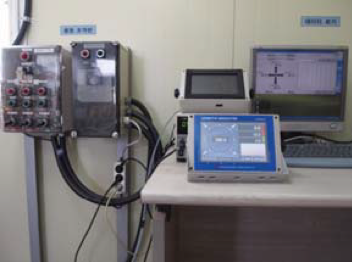
\includegraphics{fig_1}% Here is how to import EPS art
% \caption{\label{fig:epsart} A figure caption. The figure captions are
% automatically numbered.}
% \end{figure}
% is small enough to fit in a single column, while
% Fig.~\ref{fig:wide}%
% \begin{figure*}
% \includegraphics{fig_2}% Here is how to import EPS art
% \caption{\label{fig:wide}Use the \texttt{figure*} environment to get a wide
% figure, spanning the page in \texttt{twocolumn} formatting.}
% \end{figure*}
% is too wide for a single column,
% so instead the \texttt{figure*} environment has been used.

% The analog of the \texttt{figure} environment is \texttt{table}, which uses
% the same \verb+\caption+ command.
% However, you should type your caption command first within the \texttt{table}, 
% instead of last as you did for \texttt{figure}.

% The heart of any table is the \texttt{tabular} environment,
% which represents the table content as a (vertical) sequence of table rows,
% each containing a (horizontal) sequence of table cells. 
% Cells are separated by the \verb+&+ character;
% the row terminates with \verb+\\+. 
% The required argument for the \texttt{tabular} environment
% specifies how data are displayed in each of the columns. 
% For instance, a column
% may be centered (\verb+c+), left-justified (\verb+l+), right-justified (\verb+r+),
% or aligned on a decimal point (\verb+d+). 
% (Table~\ref{tab:table4}%
% \begin{table}
% \caption{\label{tab:table4}Numbers in columns Three--Five have been
% aligned by using the ``d'' column specifier (requires the
% \texttt{dcolumn} package). 
% Non-numeric entries (those entries without
% a ``.'') in a ``d'' column are aligned on the decimal point. 
% Use the
% ``D'' specifier for more complex layouts. }
% \begin{ruledtabular}
% \begin{tabular}{ccddd}
% One&Two&\mbox{Three}&\mbox{Four}&\mbox{Five}\\
% \hline
% one&two&\mbox{three}&\mbox{four}&\mbox{five}\\
% He&2& 2.77234 & 45672. & 0.69 \\
% C\footnote{Some tables require footnotes.}
%   &C\footnote{Some tables need more than one footnote.}
%   & 12537.64 & 37.66345 & 86.37 \\
% \end{tabular}
% \end{ruledtabular}
% \end{table}
% illustrates the use of decimal column alignment.)

% Extra column-spacing may be be specified as well, although
% REV\TeX~4 sets this spacing so that the columns fill the width of the
% table.
% Horizontal rules are typeset using the \verb+\hline+
% command.
% The doubled (or Scotch) rules that appear at the top and
% bottom of a table can be achieved by enclosing the \texttt{tabular}
% environment within a \texttt{ruledtabular} environment.
% Rows whose columns span multiple columns can be typeset using \LaTeX's
% \verb+\multicolumn{#1}{#2}{#3}+ command
% (for example, see the first row of Table~\ref{tab:table3}).%
% \begin{table*}
% \caption{\label{tab:table3}This is a wide table that spans the page
% width in \texttt{twocolumn} mode. It is formatted using the
% \texttt{table*} environment. It also demonstrates the use of
% \textbackslash\texttt{multicolumn} in rows with entries that span
% more than one column.}
% \begin{ruledtabular}
% \begin{tabular}{ccccc}
%  &\multicolumn{2}{c}{$D_{4h}^1$}&\multicolumn{2}{c}{$D_{4h}^5$}\\
%  Ion&1st alternative&2nd alternative&lst alternative
% &2nd alternative\\ \hline
%  K&$(2e)+(2f)$&$(4i)$ &$(2c)+(2d)$&$(4f)$ \\
%  Mn&$(2g)$\footnote{The $z$ parameter of these positions is $z\sim\frac{1}{4}$.}
%  &$(a)+(b)+(c)+(d)$&$(4e)$&$(2a)+(2b)$\\
%  Cl&$(a)+(b)+(c)+(d)$&$(2g)$\footnote{This is a footnote in a table that spans the full page
% width in \texttt{twocolumn} mode. It is supposed to set on the full width of the page, just as the caption does. }
%  &$(4e)^{\text{a}}$\\
%  He&$(8r)^{\text{a}}$&$(4j)^{\text{a}}$&$(4g)^{\text{a}}$\\
%  Ag& &$(4k)^{\text{a}}$& &$(4h)^{\text{a}}$\\
% \end{tabular}
% \end{ruledtabular}
% \end{table*}

% The tables in this document illustrate various effects.
% Tables that fit in a narrow column are contained in a \texttt{table}
% environment.
% Table~\ref{tab:table3} is a wide table, therefore set with the
% \texttt{table*} environment.
% Lengthy tables may need to break across pages.
% A simple way to allow this is to specify
% the \verb+[H]+ float placement on the \texttt{table} or
% \texttt{table*} environment.
% Alternatively, using the standard \LaTeXe\ package \texttt{longtable} 
% gives more control over how tables break and allows headers and footers 
% to be specified for each page of the table.
% An example of the use of \texttt{longtable} can be found
% in the file \texttt{summary.tex} that is included with the REV\TeX~4
% distribution.

% There are two methods for setting footnotes within a table (these
% footnotes will be displayed directly below the table rather than at
% the bottom of the page or in the bibliography).
% The easiest
% and preferred method is just to use the \verb+\footnote{#1}+
% command. This will automatically enumerate the footnotes with
% lowercase roman letters.
% However, it is sometimes necessary to have
% multiple entries in the table share the same footnote.
% In this case,
% create the footnotes using
% \verb+\footnotemark[#1]+ and \verb+\footnotetext[#1]{#2}+.
% \texttt{\#1} is a numeric value.
% Each time the same value for \texttt{\#1} is used, 
% the same mark is produced in the table. 
% The \verb+\footnotetext[#1]{#2}+ commands are placed after the \texttt{tabular}
% environment. 
% Examine the \LaTeX\ source and output for Tables~\ref{tab:table1} and 
% \ref{tab:table2}%
% \begin{table}
% \caption{\label{tab:table2}A table with more columns still fits
% properly in a column. Note that several entries share the same
% footnote. Inspect the \LaTeX\ input for this table to see
% exactly how it is done.}
% \begin{ruledtabular}
% \begin{tabular}{cccccccc}
%  &$r_c$ (\AA)&$r_0$ (\AA)&$\kappa r_0$&
%  &$r_c$ (\AA) &$r_0$ (\AA)&$\kappa r_0$\\
% \hline
% Cu& 0.800 & 14.10 & 2.550 &Sn\footnotemark[1]
% & 0.680 & 1.870 & 3.700 \\
% Ag& 0.990 & 15.90 & 2.710 &Pb\footnotemark[2]
% & 0.450 & 1.930 & 3.760 \\
% Au& 1.150 & 15.90 & 2.710 &Ca\footnotemark[3]
% & 0.750 & 2.170 & 3.560 \\
% Mg& 0.490 & 17.60 & 3.200 &Sr\footnotemark[4]
% & 0.900 & 2.370 & 3.720 \\
% Zn& 0.300 & 15.20 & 2.970 &Li\footnotemark[2]
% & 0.380 & 1.730 & 2.830 \\
% Cd& 0.530 & 17.10 & 3.160 &Na\footnotemark[5]
% & 0.760 & 2.110 & 3.120 \\
% Hg& 0.550 & 17.80 & 3.220 &K\footnotemark[5]
% &  1.120 & 2.620 & 3.480 \\
% Al& 0.230 & 15.80 & 3.240 &Rb\footnotemark[3]
% & 1.330 & 2.800 & 3.590 \\
% Ga& 0.310 & 16.70 & 3.330 &Cs\footnotemark[4]
% & 1.420 & 3.030 & 3.740 \\
% In& 0.460 & 18.40 & 3.500 &Ba\footnotemark[5]
% & 0.960 & 2.460 & 3.780 \\
% Tl& 0.480 & 18.90 & 3.550 & & & & \\
% \end{tabular}
% \end{ruledtabular}
% \footnotetext[1]{Here's the first, from Ref.~\onlinecite{feyn54}.}
% \footnotetext[2]{Here's the second.}
% \footnotetext[3]{Here's the third.}
% \footnotetext[4]{Here's the fourth.}
% \footnotetext[5]{And etc.}
% \end{table}
% for an illustration. 

% All AIP journals require that the initial citation of
% figures or tables be in numerical order.
% \LaTeX's automatic numbering of floats is your friend here:
% just put each \texttt{figure} environment immediately following 
% its first reference (\verb+\ref+), as we have done in this example file. 

% \begin{acknowledgments}
% We wish to acknowledge the support of the author community in using
% REV\TeX{}, offering suggestions and encouragement, testing new versions,
% \dots.
% \end{acknowledgments}

% \section*{Data Availability Statement}

% AIP Publishing believes that all datasets underlying the conclusions of the paper should be available to readers. Authors are encouraged to deposit their datasets in publicly available repositories or present them in the main manuscript. All research articles must include a data availability statement stating where the data can be found. In this section, authors should add the respective statement from the chart below based on the availability of data in their paper.

% \begin{center}
% \renewcommand\arraystretch{1.2}
% \begin{tabular}{| >{\raggedright\arraybackslash}p{0.3\linewidth} | >{\raggedright\arraybackslash}p{0.65\linewidth} |}
% \hline
% \textbf{AVAILABILITY OF DATA} & \textbf{STATEMENT OF DATA AVAILABILITY}\\  
% \hline
% Data available on request from the authors
% &
% The data that support the findings of this study are available from the corresponding author upon reasonable request.
% \\\hline
% Data available in article or supplementary material
% &
% The data that support the findings of this study are available within the article [and its supplementary material].
% \\\hline
% Data openly available in a public repository that issues datasets with DOIs
% &
% The data that support the findings of this study are openly available in [repository name] at http://doi.org/[doi], reference number [reference number].
% \\\hline
% Data openly available in a public repository that does not issue DOIs
% &
% The data that support the findings of this study are openly available in [repository name], reference number [reference number].
% \\\hline
% Data sharing not applicable – no new data generated
% &
% Data sharing is not applicable to this article as no new data were created or analyzed in this study.
% \\\hline
% Data generated at a central, large scale facility
% &
% Raw data were generated at the [facility name] large scale facility. Derived data supporting the findings of this study are available from the corresponding author upon reasonable request.
% \\\hline
% Embargo on data due to commercial restrictions
% &
% The data that support the findings will be available in [repository name] at [DOI link] following an embargo from the date of publication to allow for commercialization of research findings.
% \\\hline
% Data available on request due to privacy/ethical restrictions
% &
% The data that support the findings of this study are available on request from the corresponding author. The data are not publicly available due [state restrictions such as privacy or ethical restrictions].
% \\\hline
% Data subject to third party restrictions
% &
% The data that support the findings of this study are available from [third party]. Restrictions apply to the availability of these data, which were used under license for this study. Data are available from the authors upon reasonable request and with the permission of [third party].
% \\\hline
% \end{tabular}
% \end{center}

% \appendix

% \section{Appendixes}

% To start the appendixes, use the \verb+\appendix+ command.
% This signals that all following section commands refer to appendixes
% instead of regular sections. Therefore, the \verb+\appendix+ command
% should be used only once---to set up the section commands to act as
% appendixes. Thereafter normal section commands are used. The heading
% for a section can be left empty. For example,
% \begin{verbatim}
% \appendix
% \section{}
% \end{verbatim}
% will produce an appendix heading that says ``APPENDIX A'' and
% \begin{verbatim}
% \appendix
% \section{Background}
% \end{verbatim}
% will produce an appendix heading that says ``APPENDIX A: BACKGROUND''
% (note that the colon is set automatically).

% If there is only one appendix, then the letter ``A'' should not
% appear. This is suppressed by using the star version of the appendix
% command (\verb+\appendix*+ in the place of \verb+\appendix+).

% \section{A little more on appendixes}

% Observe that this appendix was started by using
% \begin{verbatim}
% \section{A little more on appendixes}
% \end{verbatim}

% Note the equation number in an appendix:
% \begin{equation}
% E=mc^2.
% \end{equation}

% \subsection{\label{app:subsec}A subsection in an appendix}

% You can use a subsection or subsubsection in an appendix. Note the
% numbering: we are now in Appendix~\ref{app:subsec}.

% \subsubsection{\label{app:subsubsec}A subsubsection in an appendix}
% Note the equation numbers in this appendix, produced with the
% subequations environment:
% \begin{subequations}
% \begin{eqnarray}
% E&=&mc, \label{appa}
% \\
% E&=&mc^2, \label{appb}
% \\
% E&\agt& mc^3. \label{appc}
% \end{eqnarray}
% \end{subequations}
% They turn out to be Eqs.~(\ref{appa}), (\ref{appb}), and (\ref{appc}).

% \nocite{*}
% \bibliography{aipsamp}% Produces the bibliography via BibTeX.

\end{document}
%
% ****** End of file aipsamp.tex ******
